\documentclass[12pt]{report}
\usepackage{geometry}
\geometry{a4paper,top=4cm,bottom=4cm,left=3cm,right=3cm,heightrounded,bindingoffset=0mm}
\usepackage[T1]{fontenc}
\usepackage[utf8]{inputenc}
\usepackage[italian]{babel}
\usepackage{lipsum}
\usepackage{url}
\usepackage{graphicx,subfigure}
\usepackage{float}
\usepackage[labelformat=empty,format=hang]{caption}
\usepackage{threeparttable}
\usepackage{latexsym}
\usepackage{wrapfig}
\usepackage{amsmath}
\usepackage{amsfonts} 
\usepackage{titling}
\usepackage{listings}
\usepackage{color} %red, green, blue, yellow, cyan, magenta, black, white
\definecolor{mygreen}{RGB}{28,172,0} % color values Red, Green, Blue
\definecolor{mylilas}{RGB}{170,55,241}
\usepackage{booktabs}
\usepackage{caption}
\usepackage{titling}
\usepackage{url}
\usepackage[export]{adjustbox}
\usepackage {hyperref} 
\usepackage{gensymb}
\usepackage{chngcntr}
\usepackage{setspace}
\usepackage{listings}
\usepackage{arydshln}
\usepackage{multirow}
\usepackage[section,below]{placeins}
\counterwithout{section}{chapter}
\hypersetup{hidelinks}
\setcounter{tocdepth}{5}



\onehalfspacing

	\newcommand{\mail}[1]{\href{mailto:#1}{\texttt{#1}}}
\newcommand{\subtitle}[1]{%
  \posttitle{%
    \par\end{center}
    \begin{center}\large#1\end{center}
    \vskip1em}%
}


\Large \title{\textit{\textbf{Testing e customizzazione del sistema POZYX collegato ad Arduino}\\ 
 \footnotesize Progetto per il Corso di Sistemi di Guida e Navigazione}}


 \author{\Large  \textbf{Sabrina Avantaggiato} \\ n\degree matricola: 490654 \\@ \mail{sabrina.avantaggiato@hotmail.it} \and \Large \textbf{Alfredo Bagalà} \\ n\degree matricola: 492473 \\ @ \mail{bagalaalfredo@gmail.com} }



\begin{document}
	\thispagestyle{empty}
	\maketitle 
	
	\thispagestyle{empty}
	\tableofcontents
	\thispagestyle{empty}
	
	\newpage
	
	\begin{section}{Obiettivi del lavoro}
		
		Il seguente elaborato si propone di analizzare il funzionamento del sistema di localizzazione Pozyx. Esso, basandosi sulla comunicazione tra antenne ultra-wideband (UWB) installate su tutti i device, fornisce informazioni relative alla posizione di un target. Nel caso specifico preso in esame, l'elemento ultimo di cui 				il sistema rileverà le coordinate (tag) viene considerato solo nella versione in cui si trova connesso ad Arduino. Punto di partenza per questo studio, è stata la documentazione Pozyx presente online e a cui si farà di seguito puntuale riferimento. L’aspetto ulteriore che però questo lavoro ha approfondito, è stato la 				connessione simultanea di due tag in comunicazione con Arduino attraverso protocollo I$^2$C. Ciò ha richiesto modifiche sia dal punto di vista hardware che software. 
		Dopo una breve presentazione del sistema Pozyx e degli strumenti utilizzati per l’analisi condotta, verranno descritte in dettaglio le prove sperimentali effettuate. In particolare, i test sono stati eseguiti sia indoor che outdoor. Per entrambe le condizioni ambientali, si è andati a ricercare la configurazione di 							parametri UWB ottimale ai fini di massimizzare update rate e aree di comunicazione. Inoltre, di tali misure, è stata valutata la precisione e l’accuratezza.

	\end{section}
	
	\begin{section}{Introduzione al sistema POZYX}

		Il sistema Pozyx è una soluzione hardware che si pone l'obiettivo di fornire informazioni accurate di posizione e di movimento di un target. Un sistema consta di 5 componenti: 4 sono dette ancore ed 1 tag. Ognuno di questi elementi integra un’antenna UWB ed altri sensori utili alla 															navigazione. Sono, infatti, presenti un accelerometro, un giroscopio, un magnetometro e un altimetro. Le due tipologie di dispositivo sono tra loro identiche, se non per il fatto che i tag presentano due pin cortocircuitati. Questo imposta, a livello hardware, un pin in pull-up il cui valore viene letto dalla scheda come 			flag per differenziarne l’utilizzo. Le ancore sono prese come riferimento e necessitano di avere posizioni relative invariate nel tempo a meno di stoppare l’esperimento e rieffettuarne la calibrazione; il tag viene montato sull’oggetto, potenzialmente in movimento, del quale si richiedono informazioni. La tecnologia su 		cui si basano questi dispositivi è un nuovo tipo di comunicazione wireless, per l'appunto l'UWB, la quale si propone di essere molto più efficace dei tradizionali sistemi. In particolare, il modulo UWB da solo rende possibile un'accurata misura dei dati. Inoltre, grazie agli algoritmi di Pozyx relativi al 	ranging e al 					positioning, implementati sul microcontrollore (MCU),  è possibile ricevere delle misure con un errore complessivo dichiarato di circa $10 cm$. Un'ulteriore caratteristica, fondalmentale ai fini del seguente lavoro, è la predisposizione dei tag ad essere collegati ad un modulo Arduino. Infatti, sono progettati per 					essere una shield per Arduino Uno Rev3, garantendo una piena compatibilità con esso. Uno schema riassuntivo del modo in cui sensori, MCU, UWB e connessione ad Arduino sono integrate è presente in \textbf{\figurename~\ref{Fsisttag}}.

		\begin{figure}[h]
			\centering
			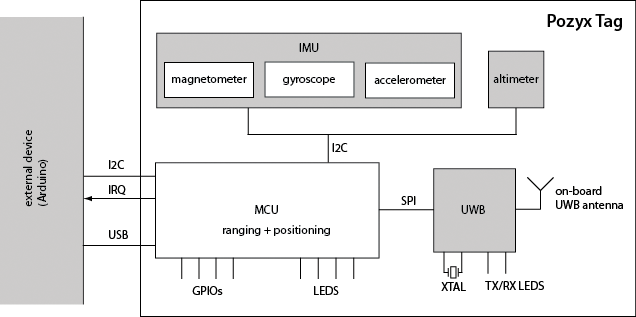
\includegraphics[scale=0.5]{system_tag}
	 		\caption{\textbf{Figura 1:} Tag Pozyx}\label{Fsisttag}
		\end{figure}

	\begin{subsection}{Utilizzo}
		
		Come già enunciato precedentemente, ai fini del lavoro in esame, viene preso in considerazione il funzionamento del sistema collegato ad un Arduino Uno Rev3. Per poter far funzionare il sistema, innanzitutto, bisogna scaricare la libreria fornita da Pozyx$^{{\cite{cit1}}}$ ed includerla tra le librerie di Arduino. 				Una volta scaricata, deve essere inserita nella cartella $C:\setminus...\setminus Arduino\setminus libraries$ oppure, direttamente dal software fornito da Arduino$^{{\cite{cit2}}}$, bisogna digitare su $Sketch>\#includi$ $libreria>Aggiungi$ $libreria$ $da$ $file .ZIP…$ e selezionare la cartella (Pozyx), in formato 			ZIP.\\
		Per utilizzare	correttamente il set di dispositivi ci si rifà alle regole che vengono riportate nella documentazione$^{{\cite{cit3}}}$ e sintetizzate di seguito.

	\end{subsection}

	\begin{subsection}{Come posizionare le ancore}

		Per un corretto posizionamento delle ancore ci si basa su 4 semplici regole:

		\begin{enumerate}
				\item posizionarle in alto, in modo che tra tag e ancore intercorrano meno ostacoli possibili;
				\item posizionarle in ordine sparso, in particolare non tutte allineate per evitare che l’algoritmo di trilaterazione fallisca;
				\item posizionare ancore e tag verticalmente, come in \textbf{\figurename~\ref{Fanchor}}, con l'antenna UWB posta nella parte superiore. Risulta, infatti, impossibile costruire dispositivi che irradino con la stessa potenza di segnale in tutte le direzioni. Con riferimento alla stessa figura, le apparecchiature 									 Pozyx sono omnidirezionali sul piano xz, ma non lungo l’asse y;
				\item per il riconoscimento della posizione di un tag nello spazio tridimensionale è necessario che le ancore non siano tutte sullo stesso piano orizzontale. Quindi, almeno un'ancora, dovrà essere installata ad un'altezza diversa dalle altre tre.
		\end{enumerate}

		\begin{figure}[h]
			\centering
			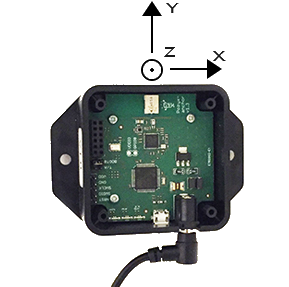
\includegraphics[scale=1.8]{anchor_placement}
	 		\caption{\textbf{Figura 2:} Corretto posizionamento di una singola ancora}\label{Fanchor}
		\end{figure}

	\end{subsection}

	\begin{subsection}{Come funziona l'Ultra-wideband}

		I dispositivi UWB comunicano tramite onde radio, le quali viaggiano alla velocità della luce ($c=299792458m/s$). Una volta che il ricevitore ha, per l’appunto, ricevuto il segnale dall’emettitore ha due modi per risalire all’informazione sulla distanza che intercorre tra i due:

		\begin{itemize}
				\item calcolare la differenza di potenza tra il segnale inviato e quello ricevuto; 
				\item misurare il tempo di volo del segnale.
		\end{itemize}
		Il primo dei due metodi non è utilizzabile in questo caso per due ragioni. Esso richiede segnali ad elevata potenza rispetto a quella utilizzata ed inoltre il segnale in arrivo sarebbe corrotto da riflessioni su tutti gli oggetti del percorso, rendendo la misura finale probabilmente poco accurata in ambienti chiusi. Viene, 				invece, utilizzato il secondo di questi metodi inviando un’onda radio e misurandone il tempo di volo all'arrivo. Conoscendo la velocità a cui viaggia il segnale, si ottiene la distanza come $d = c* \Delta t$. Secondo il principio di inderminazione di Heisemberg, però, non è possibile conoscere contemporaneamente 				frequenza e timing di un segnale. Utilizzando la seguente disuguaglianza:

		\begin{equation}
			\Delta f\Delta t \ge \frac{1}{4\pi},      
		\end{equation}
		si nota che per conoscere un $\Delta t$ più piccolo bisogna avere una $\Delta f$ (banda passante del segnale) il più possibile ampia. Per esempio il $\Delta f$ del wifi è pari a $20MHz$, cioè è possibile discriminare distanze superiori a $1.2 m$. Le UWB prendono il loro nome, ed anche la loro caratteristica di 						accuratezza, proprio dal fatto che la loro $\Delta f = 500MHz$, il che rende possibile misurare tempi fino a $0.16 ns$. Questo perché il segnale inviato dalle UWB è un segnale a bassissima potenza (la densità spettrale di potenza deve essere inferiore a $-41.3dBm/MHz$). Ciò rende tali dispositivi utilizzabili in un 				range circoscritto di distanze.

	\end{subsection}

	\begin{subsection}{Come funziona il \textit{positioning}$^{{\cite{cit5}}}$}
		
		Per identificare la posizione di un oggetto c’è bisogno di due elementi:

		\begin{itemize}
				\item le misure;
				\item alcuni punti di riferimento.
		\end{itemize}

		Nel caso dei sistemi Pozyx, le misure sono le distanze tra il tag e le ancore e i punti di riferimento sono le posizioni delle ancore stesse.\\
		In genere il modo più semplice per risolvere il problema del posizionamento è l'utilizzo di semplici conoscenze geometriche. Infatti, il metodo più comune è quello della trilaterazione. Esso si fonda sul fatto che, se abbiamo a disposizione una misura della distanza tra un punto di riferimento e il target, 								quest’ultimo si possa trovare su una circonferenza (o una sfera in 3D) di raggio pari alla distanza. Se, però, avessimo a disposizione 4 di queste distanze da 4 punti di riferimento differenti e noti, l’intersezione di tutte le circonferenze identificherebbe il punto in cui realmente si trova il target. La stima delle 							coordinate è il risultato di un'ottimizzazione traminte l'algoritmo ai minimi quadrati.
 
	\end{subsection}

	\begin{subsection}{Sistema di Riferimento (SdR)}

		Le ancore rappresentano i punti di riferimento nel sistema Pozyx. Inoltre, risulta rilevante anche la successione con cui esse vengono impostate a livello software. Per convenzione, la prima ancora definisce l’origine degli assi. L'asse \textit{y} ha come direzione la retta passante per la posizione delle prime due 					ancore e il verso positivo è quello entrante nella seconda ancora. L’asse \textit{z} è sempre preso verso l’alto e di conseguenza l’asse \textit{x} sarà scelto in modo che il Sistema di Riferimento (SdR) formi una terna-levogira.

	\end{subsection}

	\begin{subsection}{Parametri}

		\hypertarget{SS4}{Ogni} dispositivo del sistema Pozyx è caratterizzato da un insieme di parametri UWB, impostabili dall’utente. Affinchè possa avvenire la comunicazione è, però, necessario che il set di parametri sia lo stesso sia per il/i tag che per le ancore.
		Essi sono così definiti:

		\begin{itemize}
			\item \textbf{channel}: questo parametro setta il canale UWB. Ogni dispositivo Pozyx può utilizzare 6 canali indipendenti (1,2,3,4,5,7), che differiscono per la frequenza di trasmissione. In particolare, canali più bassi lavorano a frequenze più basse.
			\item \textbf{bitrate}: questo parametro imposta il bitrate UWB. È possibile settare 3 diversi valori: $110kbit/s$, $850kbit/s$ e $6.81Mbit/s$. Un bitrate più elevato implica una maggiore velocità di trasmissione dei dati.
			\item \textbf{pulse repetition frequency} (\textbf{PRF}): Questo parametro imposta la frequenza degli impulsi, alla base della comunicazione UWB. È possibile scegliere tra due valori: $16MHz$ o $64MHz$. 
			\item \textbf{preamble length} (\textbf{plen}): questo parametro imposta la lunghezza del preambolo che viene posto davanti a ciascun messaggio scambiato tra i dispositivi Pozyx. Possono essere selezionati 8 differenti valori: 4096, 2048, 1536, 1024, 512, 256, 128 o 64. Un plen più 										 									piccolo corrisponde a un messaggio più breve e quindi a una comunicazione più veloce. Questo comporterà, nuovamente, una distanza di comunicazione dalle ancore limitata.
			\item \textbf{gain}: determina l’intensità degli impulsi e può assumere valori compresi tra $11.5$ e $33$ $dB$. Come verrà successivamente dimostrato, un elevato guadagno comporta un distanza di comunicazione del tag dalle ancore maggiore, a discapito dell'accuratezza delle misure.
		\end{itemize}

		Nella \hyperlink{SS1}{\textbf{sottosezione Parametri UWB}}, verrà spiegato come variare tali parametri e le conseguenze che questo comporta. Infatti, sono stati effettuati esperimenti in termini di frequenza di lavoro e di distanza di comunicazione al variare di essi.

	\end{subsection}

	\end{section}
	\newpage

	\begin{section}{Strumenti}
	
	Per lo sviluppo del progetto sono stati necessari, dal punto di vista hardware, solamente un set Pozyx con l’aggiunta di un tag (quindi 4 ancore e 2 tag) e un Arduino Uno Rev3.
	A livello software, oltre all'ambiente di programmazione Arduino, sono stati utilizzati Procesing 3 e Matlab, con scopi diversi e descritti di seguito.

	\begin{subsection}{Arduino e collegamenti circuitali}

		Arduino è una piattaforma hardware composta di una serie di schede elettroniche dotate di un microcontrollore a 8-bit AVR prodotto dalla Atmel. Si basa su un circuito stampato$^{{\cite{cit7}}}$ che integra un microcontrollore con dei pin connessi alle porte I/O, un regolatore di tensione e, in alcuni modelli, 					un'interfaccia USB che permette la comunicazione con il computer utilizzato per programmare. Assieme all’hardware viene prodotto un software che consiste in un ambiente di sviluppo integrato$^{{\cite{cit2}}}$ (IDE) disponibile per Linux, Apple Macinthosh e Windows.\\
		Arduino Uno Rev 3, che è stato il modello utilizzato durante questo lavoro per la sua piena compatibilità col sistema Pozyx, presenta le caratteristiche riportate in \textbf{\tablename~\ref{TArduinoUno}}$^{{\cite{cit7}}}$.

		\begin{table}[h]
			\centering
			\begin{tabular}{|ll|}
				\hline
				Microcontroller& 						ATmega328\\
				Operating Voltage&					5V\\
				Input Voltage&							7-12V\\
				Input Voltage (limit)&				6-20V\\
				Digital I/O Pins&						14 (6 dei quali con output PWM)\\
				PWM Digitall I/O Pins&				6\\		
				Analog Input Pins&					6\\
				DC Current per I/O Pin&				20mA\\
				DC Current for 3.3V Pin&			50mA\\
				Flash Memory&							32 KB (ATmega328P) (0.5KB usati come bootloader)\\	
				SRAM&										2 KB (ATmega328P)\\
				EEPROM&									1 KB (ATmega328P)\\
				Clock Speed&							16MHz\\
				LED BUILTIN&							13\\
				Lunghezza&								68.6 mm\\
				Larghezza&								53.4 mm\\
				Peso&										25 g\\
				\hline
		   \end{tabular}
		   \caption{\textbf{Tabella 1: }Parametri caratteristici di Arduino Uno Rev3\label{TArduinoUno}}
	 	\end{table}

		In  \hyperlink{A1}{\textbf{Allegato A}} viene riportato lo schema circuitale del dispositivo.\\

		\hypertarget{S1}{I} tag della Pozyx, considerati singolarmente, sono progettati come una shield per Arduino Uno Rev3, perciò tutti i loro pin possono essere direttamente inseriti sulla scheda. Con l’idea di poter collegare due tag distanti l’uno dall’altro, cosa che verrà descritta in seguito, sono stati studiati i pin 						realmente utili al fine della connessione. Come riportato nella documentazione$^{{\cite{cit6}}}$ i pin utilizzati sono SDA-SCL, addetti alla comunicazione I$^2$C tra Arduino e tag (vedi sezione I2C); 5V e GrouND; i Pin 1 e 2 (digitali) per eventuali segnali di interruzione (\textbf{\figurename~\ref{Fanchor}}).

		\begin{figure}[h]
			\centering
			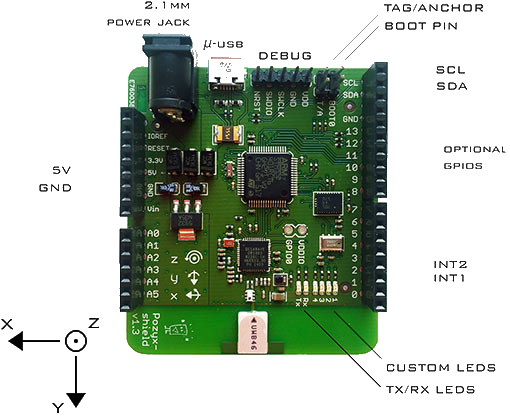
\includegraphics[scale=1.2]{pozyx_pins2}
	 		\caption{\textbf{Figura 3:} Collegamento circuitale tra arduino e tag}\label{Fpozyx_pins2}
		\end{figure}

	\end{subsection}

	\begin{subsection}{Processing 3}
	
		Processing è un software$^{{\cite{cit9}}}$ gratuito ed open-source, disponibile per Linux, Apple Macinthosh e Windows. Inizialmente ideato come sketchbook e strumento di insegnamento per le basi in un contesto visivo, si è poi evoluto fino ad essere oggi uno strumento di sviluppo professionale. Anche se non 			strettamente necessario, tale software è risultato particolarmente utile nella fase sperimentativa. Scritto un opportuno codice (riportato in \hyperlink{A2}{\textbf{Allegato B}}), è stato possibile esaminare in tempo reale qualitatamente l'andamento dell’esperimento. In particolare, le caratteristiche visualizzabili 					sono la presenza eccessiva di rumore, un'errata calibrazione, il numero di misure effettuate e la percentuale di fallimenti. Il codice è stato scritto sfruttando il fatto che il programma riesce a leggere i dati inviati su seriale da Arduino. Trascurando per il momento come questi dati vengano elaborati ed inviati, si 					tenga presente che il pacchetto di valori letti è il seguente:
		
		\begin{footnotesize}$(X,     Y,    Z,    DIST\_ANCORA0,    DIST\_ANCORA1,    DIST\_ANCORA2,    DIST\_ANCORA3)$.\end{footnotesize}

		In presenza di due tag, il pacchetto così come è riportato sopra, viene duplicato; inoltre, in alcuni esperimenti viene anche inviato su seriale un ultimo dato che rappresenta il tempo, per una sua successiva analisi. Il codice una volta lanciato, permette innanzitutto di stampare a video le 4 ancore (rappresentate dai 			4 quadratini rossi in \textbf{\figurename~\ref{Ffunzionamento_processing}}) e del sistema di riferimento. La simulazione, come illustrato in figura, consente anche di visualizzare: in basso a sinistra la scala di rappresentazione; in basso a destra un riquadro con le coordinate nel piano dei due tag, il numero di 					misure effettuate e la relativa percentuale di fallimenti. In tal modo è possibile monitorare l’eventuale presenza di eccessivo disturbo che potrebbe portare ad una mancata convergenza dell’algoritmo di positioning. Una volta che su seriale cominciano ad arrivare i dati relativi alla localizzazione dei tag, questi 						vengono stampati con due differenti colori (verde e blu); inoltre, ogni cento campioni, vengono stampati due quadrati più grandi (rispettivamente in arancio e azzurro) in modo che se i tag fossero in movimento sarebbe facile ricostruire, già graficamente, il percorso da essi descritto. Da notare come in alcuni 					esperimenti che ci sia una nuvola (iniziale) di punti delocaizzata rispetto alla reale posizione. Questo dovuto al fatto che l'algoritmo di positioning necessita di un tempo di transitorio per andare a regime. Verrà successivamente chiarito come questo aspetto è stato risolto. Il codice, inoltre, genera un file .txt. 						Non appena viene digitato un qualsiasi tasto, la simulazione si stoppa consentendo un salvataggio automatico dell’immagine al momento della chiusura e del file contenente le misure ricevute fino a quel momento.
		
		\begin{figure}[H]
			\centering
			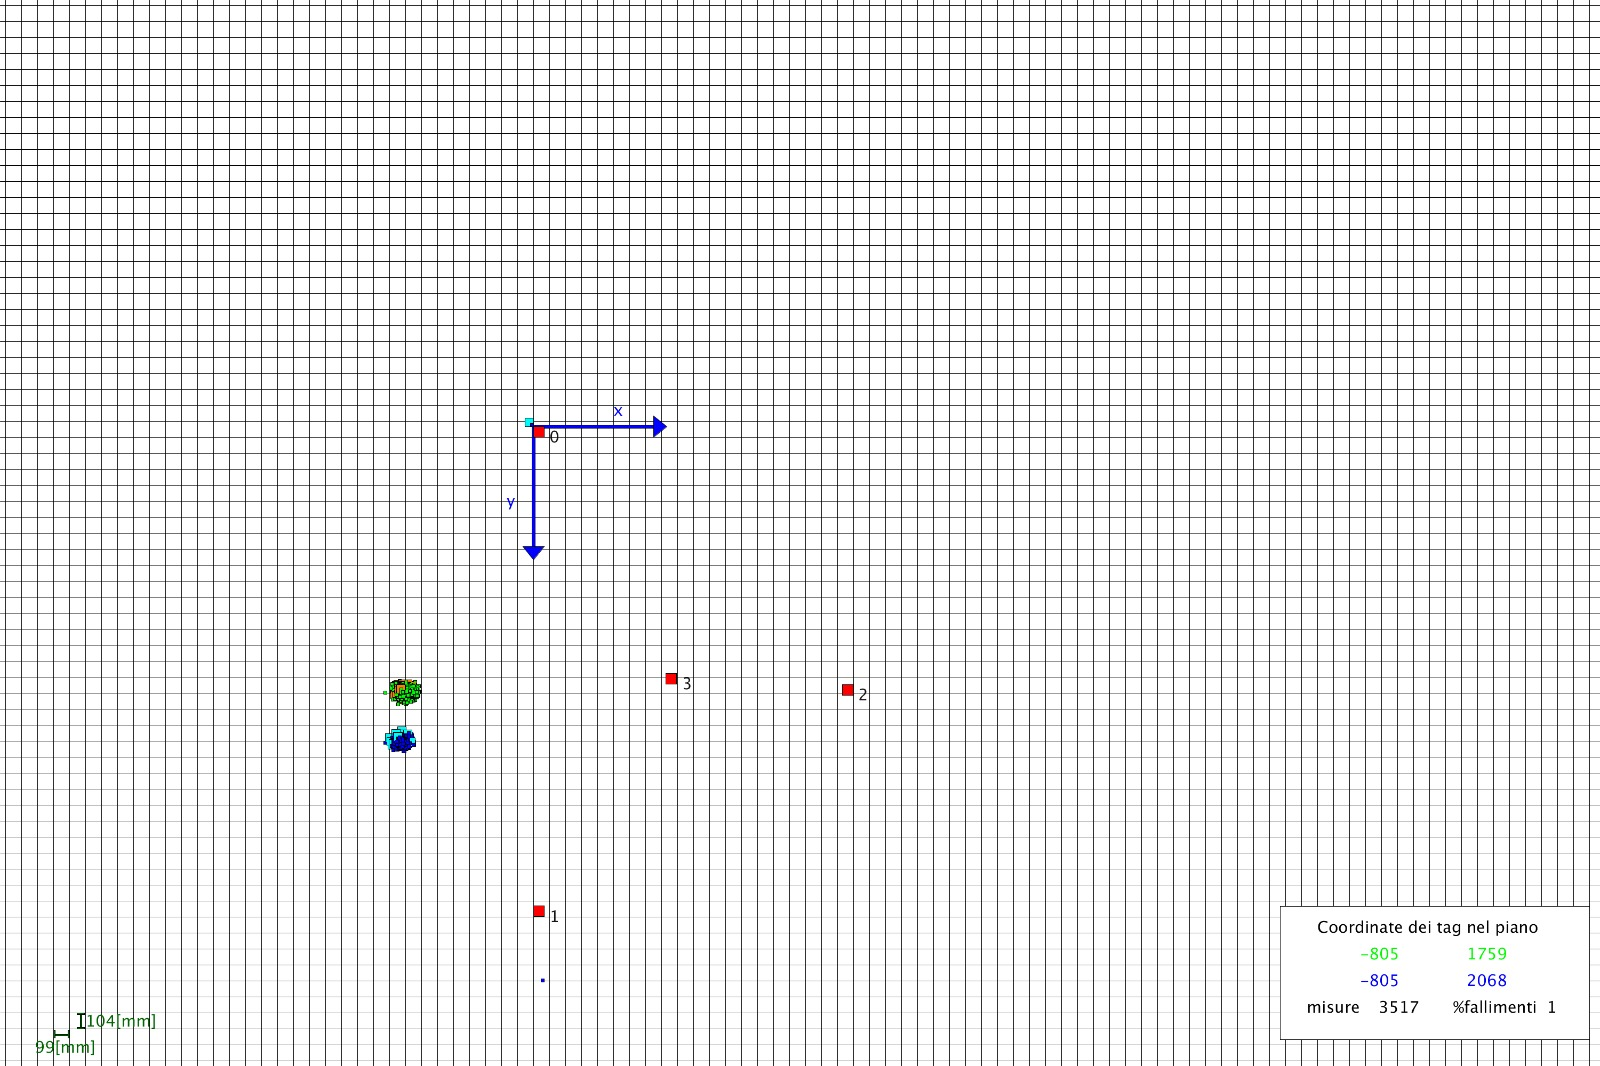
\includegraphics[scale=0.9]{processing_dimostration}
	 		\caption{\textbf{Figura 4:} interfaccia grafica processing}\label{Ffunzionamento_processing}
		\end{figure}

	\end{subsection}

	\begin{subsection}{Matlab e Simulink}

		Per questa analisi è stato utilizzato Matlab, con degli script di volta in volta adattati allo scopo dell’esperimento.\\ 
		Inoltre, è stato utilizzato uno schema Simulink già sviluppato in lavori precedenti, utile a simulare la comunicazione tra Arduino (collegato al sistema Pozyx) e l'autopilota. Tale schema è atto alla lettura da seriale di valori in formato binario. In particolare, la comunicazione inizia quando il ricevitore rileva il carattere 			di inizio stringa ("\textit{BB}"). È, inoltre, fondamentale stabilire a priori il numero di bytes che compongono la stringa. Nel nostro caso tale valore è corrispondente a $57bytes$. 

	\end{subsection}

	\end{section}
	\newpage

	\begin{section}{Comunicazione}

		I protocolli previsti per la comunicazione con il tag sono I$^2$C e USB. Essi sono descritti nella documentazione$^{{\cite{cit10}}}$. Nella configurazione tag-arduino considerata in questa sede (come riportato in \textbf{\figurename~\ref{Fardu_tag}}), Arduino è collegato tramite USB al pc su cui è installato l’IDE 		Arduino; la comunicazione tra Arduino e uno o più tag è, invece, regolata dal protocollo I$^2$C. L'IDE Arduino consente il SerialMonitor per comunicare via “seriale” con il microcontrollore.

		\begin{figure}[h]
			\centering
			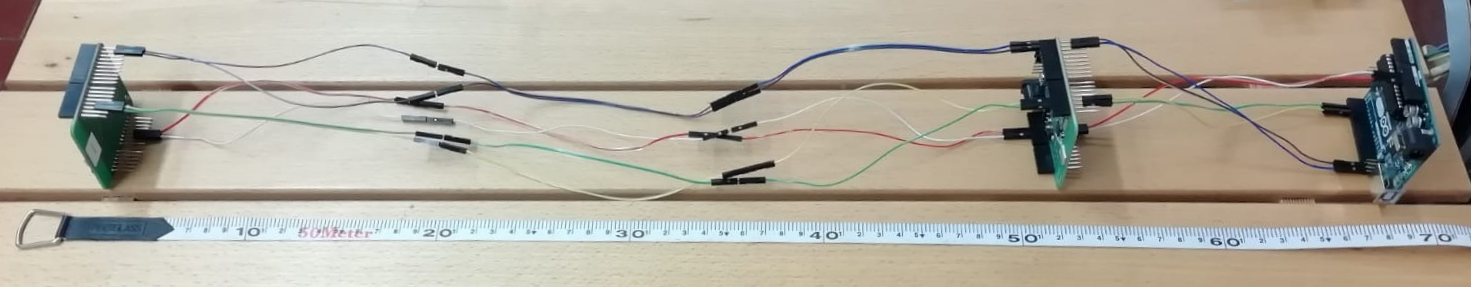
\includegraphics[scale=0.38]{ardu_tag}
	 		\caption{\textbf{Figura 5:} Collegamento tra Arduino ed i tag}\label{Fardu_tag}
		\end{figure}

		\begin{subsection}{I$^{2}$C}

			Il protocollo I$^2$C permette la comunicazione di dati tra due o più dispositivi utilizzando un bus a due fili, più uno per il riferimento comune di tensione. Le informazioni sono inviate serialmente usando una linea per i dati (SDA: Serial Data line) ed una per il Clock (SCL: Serial Clock line). Deve inoltre essere 						presente una terza linea: la massa, comune a tutti i dispositivi. 
			In questo tipo di comunicazione, i dispositivi collegati svolgono dei ruoli ben precisi: deve essere presente un Master e uno o più Slave. Il Master è un dispositivo che gestisce tutta la comunicazione controllando il segnale di clock e inviando i messaggi a tutti gli slave connessi. I dispositivi Slave 											semplicemente "ascoltano" il bus ricevendo dati dal Master o inviandone qualora questo ne faccia loro richiesta. 
			Il bus I$^2$C, basandosi su due fili, non permette la comunicazione contemporanea tra Master e Slave. Lo scambio dati deve essere gestito dal Master tramite gli indirizzi degli Slave.
			Sul bus ci può essere in ogni momento un solo Master, ma una volta terminata la comunicazione, il dispositivo Master può lasciare il suo ruolo e consentire che altri lo prendano. Il modo per selezionare un dispositivo Slave è quello di inviare il suo indirizzo sul bus di comunicazione. L’indirizzo può essere di sette 				o di dieci bit e in un sistema non ci possono essere Slave che condividono il medesimo indirizzo. \\
			Nella configurazione considerata in questo progetto, Arduino è il Master e i due tag sono gli Slave.\\
			La comunicazione su I$^2$C è gestita direttamente dalla libreria Wire fornita nell’IDE. Ogni tag è provvisto di indirizzo univoco ed è compatibile con le specifiche I$^2$C UM10204 Rev 3$^{{\cite{cit11}}}$. Secondo queste, il sistema supporta sia la modalità standard di comunicazione ($100Hz$) che 								la modalità veloce ($400Hz$) e l’indirizzo di ogni slave deve essere costituito da 7 bit. 
			L’indirizzo del tag, impostato di default, è 1001011b (0x4B). Pozyx consente di modificare l'indirizzo del tag cortocircuitando due pin, posti sul retro della scheda, denotati come "I2C LSB"; il nuovo indirizzo sarà settato a 1001010b (0x4A). 
			Per consentire la gestione dei due Slave direttamente dallo sketch di Arduino, sono state, però, necessarie modifiche alla libreria fornita da Pozyx. In particolare, è stata definita all’interno del file \textit{Pozyx\_definition.h} una variabile globale "\textit{extern unsigned char POZYX\_I2C\_ADDRESS}" che potrà 					essere inizializzata con l’indirizzo dello Slave desiderato direttamente dallo sketch. Tale variabile serve a sostituire quello che prima era un \textit{\#define} dell'indirizzo.
			Tutti gli sketch forniti consentono di utilizzare entrambi i tag shiftando tra i due indirizzi identificativi.
			A questo punto, basta collegare i due tag in blocco sulla shield di Arduino per far si che entrambi si comportino come Slave indipendenti dello stesso Master. 
			In realtà, non serve fondere i due tag e Arduino in un unico blocco impiegando tutti i pin disponibili, come anche mostrato in \textbf{\figurename~\ref{Fardu_tag}}. I pin da connettere, come anticipato nella \hyperlink{S1}{\textbf{sezione Arduino e collegamenti circuitali}}, sono: 
		
			\begin{itemize}
				\item SDA E SCL o i pin analogici A4 e A5$^{{\cite{cit12}}}$ (per la comunicazione I$^2$C);
				\item i pin (digitali) 2 e 3 (per le interruzioni);
				\item 5V e GND (per l'alimentazione).
			\end{itemize}

		\end{subsection}
	
		\begin{subsection}{Seriale}
	
		\begin{subsubsection}{Libreria Seriale di Arduino}

			\hypertarget{SS2}{Il} Sistema costituito da Arduino e dai tag, comunica con il pc attraverso la porta seriale di Arduino.  All’inizio di ogni sketch è necessario inizializzare il baud rate, cioè la velocità di trasmissione, impostata da noi sempre al valore massimo consentito da Arduino Uno e pari a \textit{115200 						bps}. Tale valore indica il numero di transazioni di bit al secondo che avvengono sulla linea. Questa è una libreria integrata di Arduino e quindi non necessita di essere inclusa negli sketch.
			Tutte le funzioni messe a disposizione dalle libreria Serial, possono essere richiamate tramite il comando: \textit{Serial.nomeDellaFunzione()}.

		 \end{subsubsection}

		 \begin{subsubsection}{Libreria SerialPort}

			\hypertarget{S2}{Nella} prima parte di questo progetto, tutti gli esperimenti sono stati condotti utilizzando la Serial fornita da Arduino. In un secondo momento, è stata scaricata e utilizzata una seconda libreria Serial\_port.h$^{{\cite{cit13}}}$. 
			La ragione di tale scelta risiede nella ricerca di un’alternativa alla Seriale standard che potesse consentire di raggiungere frequenze di lavoro più elevate.
			Per utilizzare questa seconda libreria, non basta solo scaricarla e inserirla nella cartella libraries di Arduino. Infatti, per renderla compatibile con la libreria Pozyx, è stato necessario apportarvi alcune ulteriori modifiche. In particolare è stata introdotta una variabile "\textit{extern USE\_NEW\_SERIAL}" all'interno 					del file \textit{Pozyx\_definition.h} ed, in tutti i file (\textit{Pozyx.h}, \textit{Pozyx\_lib.cpp} e \textit{Pozyx\_core.cpp}), è stata sostituita la classe \textit{Serial} con quella \textit{NewSerial}. Inoltre, in ogni sketch è necessario includere la libreria e specificare la porta seriale utilizzata 
			(\textit{USE\_NEW\_SERIAL}, \textit{USE\_NEW\_SERIAL1}, \textit{USE\_NEW\_SERIAL2} o \textit{USE\_NEW\_SERIAL3}).
			In dettaglio, nella \hyperlink{SS2}{\textbf{sottosezione SeriaPort}} relativa agli esperimenti, verranno illustrate le prove effettuate e i risultati ottenuti. Anticipiamo che non sono state riscontrate differenze sostanziali tra le due librerie relativamente alla frequenza di lavoro.
		 \end{subsubsection}

		\end{subsection}

	\end{section}
	\newpage

	\begin{section}{Introduzione alla libreria, modifiche effettuate e codice}
	
		Pozyx, oltre al sistema hardware, fornisce naturalmente un codice per la sua fruizione. Esso varia in base a come si intende interagire con i dispositivi, tramite Python o Arduino. Questo lavoro ha preso solo in considerazione l'utilizzo di Arduino. Sul sito viene riportata una documentazione													$^{{\cite{cit14}}}$, contenente il link dal quale scaricare la libreria. Al suo interno ci sono diversi esempi; in particolare la cartella \textit{useful} integra sketch utili come punto di partenza per un proprio codice.

		\begin{subsection}{Libreria POZYX}

			La libreria, nella sua esecuzione, si appoggia su altre due di Arduino: quella per la comunicazione I$^2$C e quella seriale. Analizzando il codice, si evince che per l'inizializzazione del sistema Pozyx (\textit{Pozyx.begin()}), viene utilizzato l’indirizzo del tag collegato in locale ad Arduino e definito 											all’interno del file \textit{Pozyx\_definition.h}. Si avvia, quindi, la comunicazione I$^2$C attraverso la libreria Wire.h. 
			Poichè lo scopo è quello di fornire posizione del tag e distanze dalle singole ancore, sono state nello specifico analizzate le funzioni che consentono di ottenere queste informazioni. 
			I primi dati vengono forniti attraverso la funzione \textit{doPositioning(coordinates\_t *position, uint8\_t dimension, int32\_t height)}. Essa pretende come primo ingresso un puntatore a \textit{coordinates\_t}, struttura definita dalla Pozyx come segue:\\
			\textit{struct \_\_attribute\_\_((packed))\_coordinates \{\\
    		/** Coordinata x in mm */\\
   			int32\_t x;\\
    		/** Coordinata y in mm */\\
   			int32\_t y;\\
   			 /** Coordinata z in mm */\\
  			int32\_t z;\\
			\}coordinates\_t}.\\

			All’interno di tale struttura verranno inserite le coordinate calcolate del tag, aggiornate ad ogni chiamata della funzione.\\
			Il secondo ingresso rappresenta la dimensione dello spazio in cui si muove il tag. Può essere $2.5D$, cioè l’algoritmo calcola la posizione del tag su di un piano con altezza  fissata e pari al terzo ingresso (\textit{heigth}); oppure $3D$, in cui anche la coordinata \textit{z} sarà un'incognita del positioning. La 						funzione restituisce un intero che rappresenta l'esito dell’algoritmo (1 se va a buon fine, 0 altrimenti).\\ 
			Per una descrizione più sistematica e completa del \textit{doPositiong}, si rimanda al flowchart (\hyperlink{A3}{\textbf{Allegato C}}). In esso sono state messe in particolare evidenza le comunicazioni di lettura/scrittura che avvengono tra Arduino ed il tag su bus I$^2$C ad ogni chiamata della funzione. 							Queste, infatti, rappresentano le operazioni fondamentali da sostituire qualora si voglia bypassare Arduino e collegare il/i tag direttamente ad un’altro microcontrollore.\\
			La seconda informazione, quella relativa alle distanze, viene reperita attraverso la funzione \textit{getDeviceRangeInfo(uint16\_t device\_id, device\_range\_t *device\_range, uint16\_t remote\_id)}. Essa non lancia direttamente un algoritmo di calcolo delle distanze, bensì le richiede al dispositivo specificato 					nell'ingresso \textit{device\_id}. Il risultato della chiamata viene salvato nel \textit{device\_range}, il cui indirizzo viene fornito come secondo ingresso e definito come: \\
			\textit{struct \_\_attribute\_\_((packed))\_device\_range \{\\
    		/**  Il timestamp in ms della misura del range. */\\
    		uint32\_t timestamp;\\
    		/** La distanza in mm. */\\
    		uint32\_t distance;\\
    		/** La potenza del segnale ricevuto in dBm. */\\
   			int16\_t RSS;\\
			\}device\_range\_t}.\\ 
			Il terzo ingresso è opzionale e indica l'id di un eventuale tag remoto rispetto al quale calcolare le distanze.  Non viene preso in considerazione questo caso nel lavoro in esame.

		\end{subsection}

		\begin{subsection}{Modifiche alla libreria per la gestione di due tag}

			Nell’ottica di utilizzare il sistema Pozyx con due tag contemporaneamente, la prima modifica alla libreria è stata quella di rendere l’indirizzo (\textit{POZYX\_I2C\_ADDRESS}), una variabile. In particolare:

			\begin{itemize}
				\item in \textit{Pozyx\_definition.h}: \textit{\#define POZYX\_I2C\_ADDRESS} viene sostituito da \textit{extern unsigned char POZYX\_I2C\_ADDRESS}
				\item in \textit{Pozyx\_core.cpp}: viene aggiunto nella sezione \textit{extern ‘C’}, \textit{unsigned char POZYX\_I2C\_ADDRESS}.
				\item vengono sostituiti i comandi riguardanti la porta seriale standard con i corrispettivi spiegati nella \hyperlink{S2}{\textbf{sezione Libreria SeriaPort}}.
			\end{itemize}
			La prima di queste modifiche implica che nello sketch di Arduino l’indirizzo andrà dichiarato prima del begin della piattaforma Pozyx.

		\end{subsection}

		\begin{subsection}{Codice Arduino}

			I codici utilizzati presentano un corpo comune, di seguito descritto. Si fa riferimento all' \hyperlink{A4}{\textbf{Allegato D}}.\\ 
			La prima parte è classica: riguarda l’inclusione di tutte le librerie necessarie e andrà inserita in ogni sketch. Successivamente nel codice, sono definiti tutti i parametri utilizzati. Inoltre, è stata realizzata una \textit{struct dati} che raggruppa tutti i dati di interesse relativi ad un singolo tag. Alcune 											variabili sono di facile comprensione, ma soffermandoci sugli array \textit{anchors\_x}, \textit{anchors\_y} ed \textit{heigth}, essi conterranno il risultato della calibrazione. Il processo di calibrazione fornisce le coordinate delle ancore nel SdR Pozyx. Esso rappresenta una fase preliminare alla localizzazione del 					tag, effettuabile lanciando un codice \textit{python}, già implementato e preso come punto di partenza di questo lavoro. Nella versione finale dello sketch tale operazione non è più necessaria. Infatti, una volta effettuata la calibrazione che salva in ogni ancora le sue coordinate, è già possibile lanciare il codice 					arduino. In esso è stata implementata una funzione che richiede tali informazioni alle ancore e riempie i vettori appena nominati automaticamente.\\
			Il	\textit{ranging\_protocol} ed  \textit{algorithm} selezionano due algoritmi, il primo per il ranging ed il secondo per il positioning. Mentre il primo, però, è bene non venga modificato se non a scapito di una diminuizione della frequenza di lavoro, al secondo può essere assegnato 
			\textit{POZYX\_POS\_ALG\_TRACKING} qualora il tag fosse installato su di un oggetto in movimento a velocità sostenuta. \\
			Il \textit{void setup} di Arduino contiene tutte le inizializzazioni. Innanzitutto, viene inizializzata la seriale della libreria SerialPort al baundrate massimo consentito da Arduino Uno; dopo viene assegnato il valore dell’indirizzo I$^2$C del tag con il quale Arduino comunicherà. Si ricorda che, avendo eliminato il 						define di tale parametro nell'headerfile, sarà necessario specificarlo prima che avvenga qualsiasi tipo di comunicazione tra Arduino ed il tag. A questo punto, il sistema Pozyx può essere inizializzato. Le righe di codice successive, che vengono ripetute per ogni indirizzo, servono per impostare i 	protocolli ed il 						network (gli id delle ancore). Il settaggio del clock della libreria Wire è stato già precedentemente analizzato, ma va sottolineato che, nei primi esperimenti effettuati, questa modifica non era ancora stata apportata. Le funzioni poi richiamate sono, fondamentalmente, quelle del \textit{doPositioning()} e del 						\textit{getDeviceRangeInfo()} (quest’ultima racchiusa nella funzione \textit{getDistance()} che semplicemente la richiama tante volte quante sono il numero di ancore e salva il risultato all’interno della struttura \textit{dati}). Una notazione da fare è che anche nel setup, nella versione finale, sono state aggiunte 				delle righe di codice che richiedono il positioning dei tag per un tempo prefissato. Questo perchè alla funzione \textit{doPositioning()} è necessario un tempo di circa $100ms$ per andare a regime. In questo modo, si evita di inviare su seriale i dati ottenuti durante il transitorio. Infine, va specificato come in 						questa versione, sia stata utilizzata la funzione \textit{NewSerial.write()} per inviare i valori in formato binario. In altri esperimenti questa funzione è stata sostituita dal \textit{NewSerial.print()}.

		\end{subsection}

	\end{section}
	\newpage

	\begin{section}{Esperimenti indoor}

		Al fine di verificare la precisione, l’accuratezza e la frequenza di lavoro del sistema Pozyx, sono stati condotti differenti esperimenti. Si è cercato di creare diverse condizioni di lavoro, immergendo il sistema prima in contesti chiusi, con la presenza di eventuali disturbi, e successivamente in ambienti aperti.

		Dal punto di vista hardware è stato considerato, inizialmente, un solo tag collegato sulla board di Arduino, per poi aggiungerne al sistema uno ulteriore. Nel momento in cui sono collegati entrambi i tag ad Arduino, essi risultano lavorare in parallelo come due Slave dello stesso Master. Inoltre, le condizioni 						ambientali e le posizioni degli elementi Pozyx rimangono invariate fino al termine di ogni esperimento.

		\begin{subsection}{Studio della frequenza di lavoro}

			L’obiettivo di questa serie di esperimenti consiste nel calcolo dell’update rate delle istruzioni utilizzate negli sketch. In particolare, si è cercato sia di testare la veridicità dei risultati riportati nella documentazione Pozyx$^{{\cite{cit15}}}$ che di estendere l'analisi al caso di utilizzo contemporaneo di due tag.

		\begin{subsubsection}{Variazione Clock di sincronizzazione del bus I$^2$C}

			Il primo esperimento effettuato, ha esaltato l’importanza di settare la massima velocità della comunicazione I$^2$C se si vuole lavorare con elevate frequenze di lavoro. Infatti, la libreria Wire.h di Arduino permette di scegliere tra la modalità standard pari a $100kHz$ e la modalità veloce pari a $400kHz$. 						Sono entrambe supportate da Pozyx$^{{\cite{cit16}}}$. Dunque, lasciando invariate le posizioni dei dispositivi e le condizioni ambientali nelle quali l’intero sistema è posto, è stata variata la velocità di comunicazione; questo è possibile inserendo nel \textit{void setup()} dello sketch Arduino, l’istruzione 							\textit{Wire.setclock(400000)}. L'impostazione a $100kHz$ è settata di default. 
			Per frequenza di lavoro intendiamo l’intervallo di tempo che intercorre tra due aggiornamenti delle misure di coordinate e/o distanze dalle ancore. Al fine di calcolare questo valore, sono state seguite due strade. La prima consiste nell’esaminare la durata della sola istruzione; invece, la seconda ha valutato la 						durata dell’esecuzione dell’intero ciclo, accumulando quindi anche il tempo impiegato nel richiamare il loop stesso. In questa sezione non viene preso in considerazione lo stampaggio dei dati su seriale, anche se, valutando separatamente il tempo di esecuzione della singola istruzione \textit{print()}, esso risulta 				essere praticamente ininfluente ai fini del calcolo. Quindi, la velocità di aggiornamento delle misure dipende altamente dalla velocità del loop di Arduino, oltre che alla durata di esecuzione dell'algoritmo Pozyx. La ragione per cui sono state considerate ed esaminate entrambe queste strade è di voler riprodurre la  			frequenza di aggiornamento riportata dalla documentazione. L’azienda produttrice, infatti, dichiara di poter raggiungere frequenze di lavoro pari a $140 Hz$ utilizzando una precisa combinazione di parametri UWB ($\textbf{bitrate} = 6.810Mbps$, $\textbf{channel} =5$, $\textbf{prf} =64$, $\textbf{plen}= 					64$) e settando l’algoritmo di ranging alla modalità fast. Dai nostri esperimenti, si evince che ci si può avvicinare a tale valore solamente senza considerare il tempo accumulato per richiamare il loop stesso. 
			Le istruzioni, delle quali è stata calcolata la durata con e senza loop, sono quelle utilizzate negli sketch, ovvero: \textit{doPositioning} e \textit{doRanging}, con l'eventuale aggiunta del \textit{getDeviceRangeInfo}.
			Si ricorda che il \textit{doPositioning} calcola le coordinate del tag immerso nel sistema di localizzazione Pozyx, dopo che tale sistema ha eseguito il processo di trilaterazione. Quest’ultima procedura ricava le coordinate del tag a partire dalle quattro distanze tag-ancora. Inoltre, se desiderato, é possibile 							ottenere il valore delle distanze calcolate chiamando l’istruzione \textit{getDeviceRangeInfo} e passando come argomento la singola ancora. Quindi, se l’obiettivo è quello di ottenere tutte e quattro le distanze bisogna eseguire tale istruzione altrettante volte.
			\textit{doRanging} restituisce la distanza tra tag e ancora i-esima. Di nuovo, per ottenere le quattro distanze, è necessario lanciare la funzione per quattro volte. 
			Nelle tabelle sottostanti sono riportati i valori di frequenza ottenuuti e relativa deviazione standard. Ogni valore statistico è stato ottenuto analizzando circa 1 minuto e mezzo di esecuzione dello sketch. Sono inoltre stati trascritti i massimi e i minimi valori di frequenza raggiunti da ogni prova.
			La \textbf{\tablename~\ref{Tfreqpos}} si riferisce alla frequenza ottenuta chiamando la funzione di localizzazione \textit{doPositioning} utilizzando un solo tag. È facile intuire che alla velocità di comunicazione I$^2$C più elevata corrisponde un aumento della frequenza di lavoro. Inoltre, inserendo nel calcolo la 			durata del loop, la frequenza di lavoro diminuisce di circa $10Hz$  se la velocità di comunicazione è settata a $400kHz$; diminuisce di circa 5Hz, se il bus trasferisce dati alla velocità più bassa. 			In \textbf{\tablename~\ref{Tfreqrang}}, sono illustrati i risultati del calcolo della frequenza di lavoro utilizzando la 			funzione \textit{doRanging}. Qui è stato lanciato un solo \textit{doRanging}, quindi verrà stampata solamente una distanza.
			\begin{table}[H]
				\centering
				\begin{tabular}{|lcc|r|c|c|c|}
					\hline
					\multicolumn{7}{|c|}{}\\
					\multicolumn{7}{|c|}{\textbf{\Large Frequenza di lavoro [Hz]}}\\
					\multicolumn{7}{|c|}{}\\
					\hline
					\multicolumn{4}{|l|}{}&																							Prova 1&					Prova 2&					Prova 3\\
					\hline
					{\textbf{doPositioning (400)}}&	 \multicolumn{3}{l|}{}&											140$\pm$30&			138$\pm$26&			132$\pm$29\\
					\hline
					 &	 & &							 MAX:&																					283&							558&							551\\
					\hline
					 &	 & &							 MIN:&																					71&							77&							71\\
					\hline
					{\textbf{doPositioning (400) + f\textsubscript{loop}}}&	 	\multicolumn{3}{l|}{}&		129$\pm$25&			127$\pm$22&			121$\pm$24\\
					\hline
					 &	 & &							 MAX:&																					241&							414&							412\\
					\hline
					 &	 & &							 MIN:&																					68&							73&							68\\
					\hline
					{\textbf{doPositioning (100)}}&	 \multicolumn{3}{l|}{}&											90$\pm$12&				96$\pm$9&				90$\pm$12\\
					\hline
					 &	 & &							 MAX:&																					113&							113&							113\\
					\hline
					 &	 & &							 MIN:&																					62&							68&							62\\
					\hline
					{\textbf{doPositioning (100) + f\textsubscript{loop}}}&	 	\multicolumn{3}{l|}{}&		85$\pm$11&				90$\pm$8&				85$\pm$1\\
					\hline
					 &	 & &							 MAX:&																					105&							105&							105\\
					\hline
					 &	 & &							 MIN:&																					59&							64&							59\\
					\hline
				\end{tabular}
				\caption{\textbf{Tabella 2: } Frequenza di lavoro al variale del clock del bus I$^2$C\label{Tfreqpos}}
			\end{table}	
 
			\begin{table}[H]
				\centering
				\begin{tabular}{|lcc|r|c|c|c|}
					\hline
					\multicolumn{7}{|c|}{}\\
					\multicolumn{7}{|c|}{\textbf{\Large Frequenza di lavoro [Hz]}}\\
					\multicolumn{7}{|c|}{}\\
					\hline
					\multicolumn{4}{|l|}{}&																							Prova 1&					Prova 2&					Prova 3\\
					\hline
					{\textbf{doRanging (400)}}&	 \multicolumn{3}{l|}{}&												271$\pm$1&				271$\pm$1&				271$\pm$0\\
					\hline
					 &	 & &							 MAX:&																					272&							272&							272\\
					\hline
					 &	 & &							 MIN:&																					231&							231&							269\\
					\hline
					{\textbf{doRanging (400) + f\textsubscript{loop}}}&	 	\multicolumn{3}{l|}{}&			232$\pm$1&				232$\pm$1&				232$\pm$1\\
					\hline
					 &	 & &							 MAX:&																					238&							236&							235\\
					\hline
					 &	 & &							 MIN:&																					203&							202&							228\\
					\hline
					{\textbf{doRanging (100)}}&	 \multicolumn{3}{l|}{}&												216$\pm$17&			217$\pm$1&				217$\pm$0\\
					\hline
					 &	 & &							 MAX:&																					226&							224&							225\\
					\hline
					 &	 & &							 MIN:&																					168&							169&							216\\	
					\hline
					{\textbf{doRanging (100) + f\textsubscript{loop}}}&	 	\multicolumn{3}{l|}{}&			191$\pm$13&			192$\pm$1&				191$\pm$1\\
					\hline
					 &	 & &							 MAX:&																					200&							197&							197\\
					\hline
					 &	 & &							 MIN:&																					152&							154&							189\\
					\hline
				\end{tabular}
				\caption{\textbf{Tabella 3: } Frequenza di lavoro al variale del clock del bus I$^2$C\label{Tfreqrang}}
			\end{table}	
			La frequenza massima raggiunta è pari a $272 Hz$, che corrisponde ad una durata di circa $3.6 ms$.
			I valori ricavati attraverso queste prove sono stati confrontati con quelli presenti sulla documentazione e riportati in \textbf{\figurename~\ref{Fdur_pozyx}} e in \textbf{\figurename~\ref{Fdur_pos}}. Probabilmente, l’azienda produttrice ha trascritto le frequenze ottenute trascurando la durata del loop. Infatti la 			frequenza riportata per il \textit{doPositioning} è pari a $140 Hz$  e la durata relativa al \textit{doRanging} sembra circa $3ms$. 	
			
			\begin{figure}[h]
				\centering
				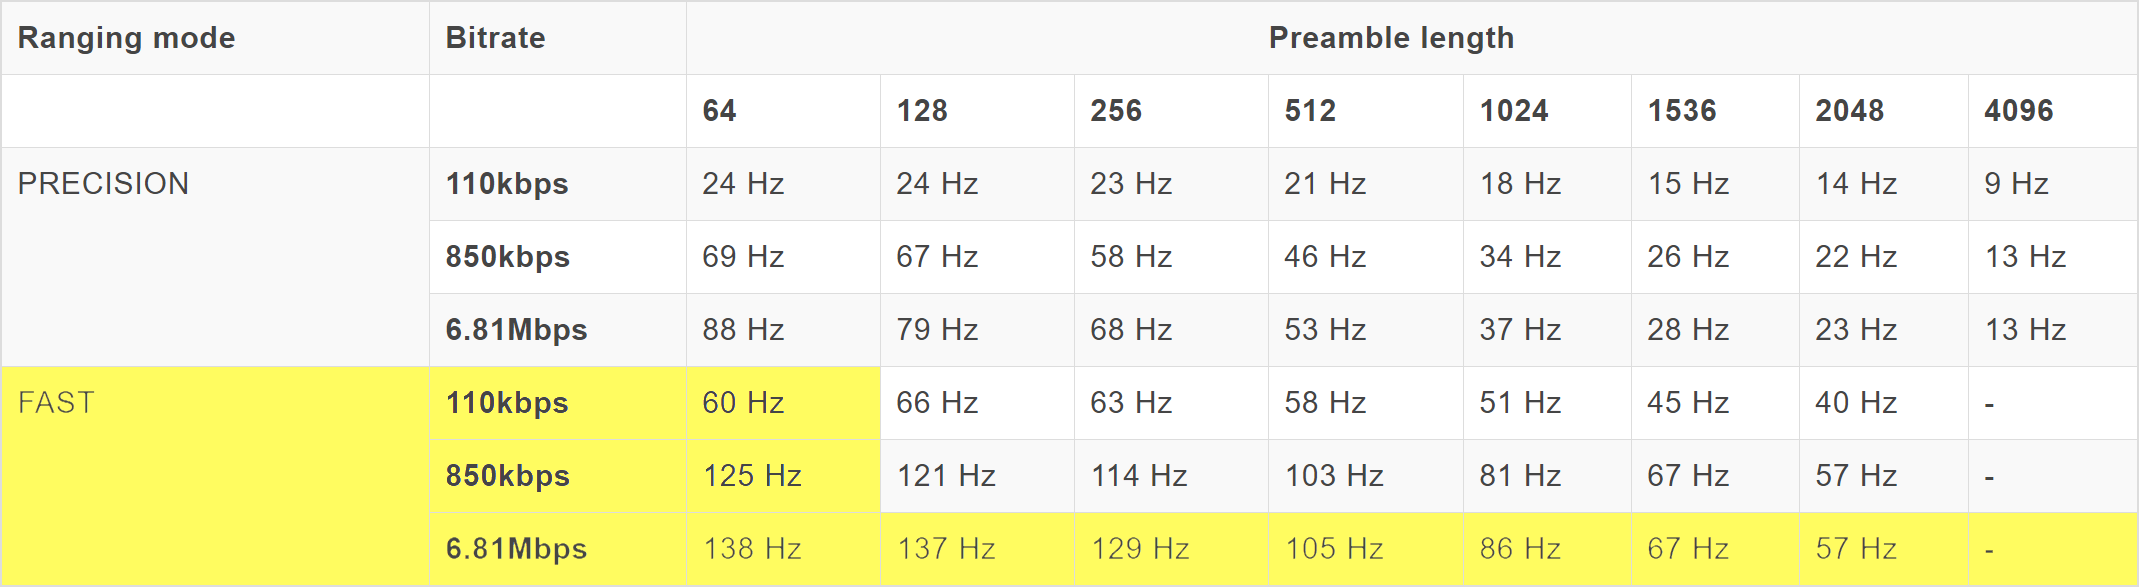
\includegraphics[scale=0.26]{pozyx_doPos_freq}
	 			\caption{\textbf{Figura 6:} Frequenza di lavoro del \textit{doPositioning} al variare dei Parametri UWB, tratto dal sito Pozyx}\label{Fdur_pos}
			\end{figure}

			\begin{figure}[h]
				\centering
				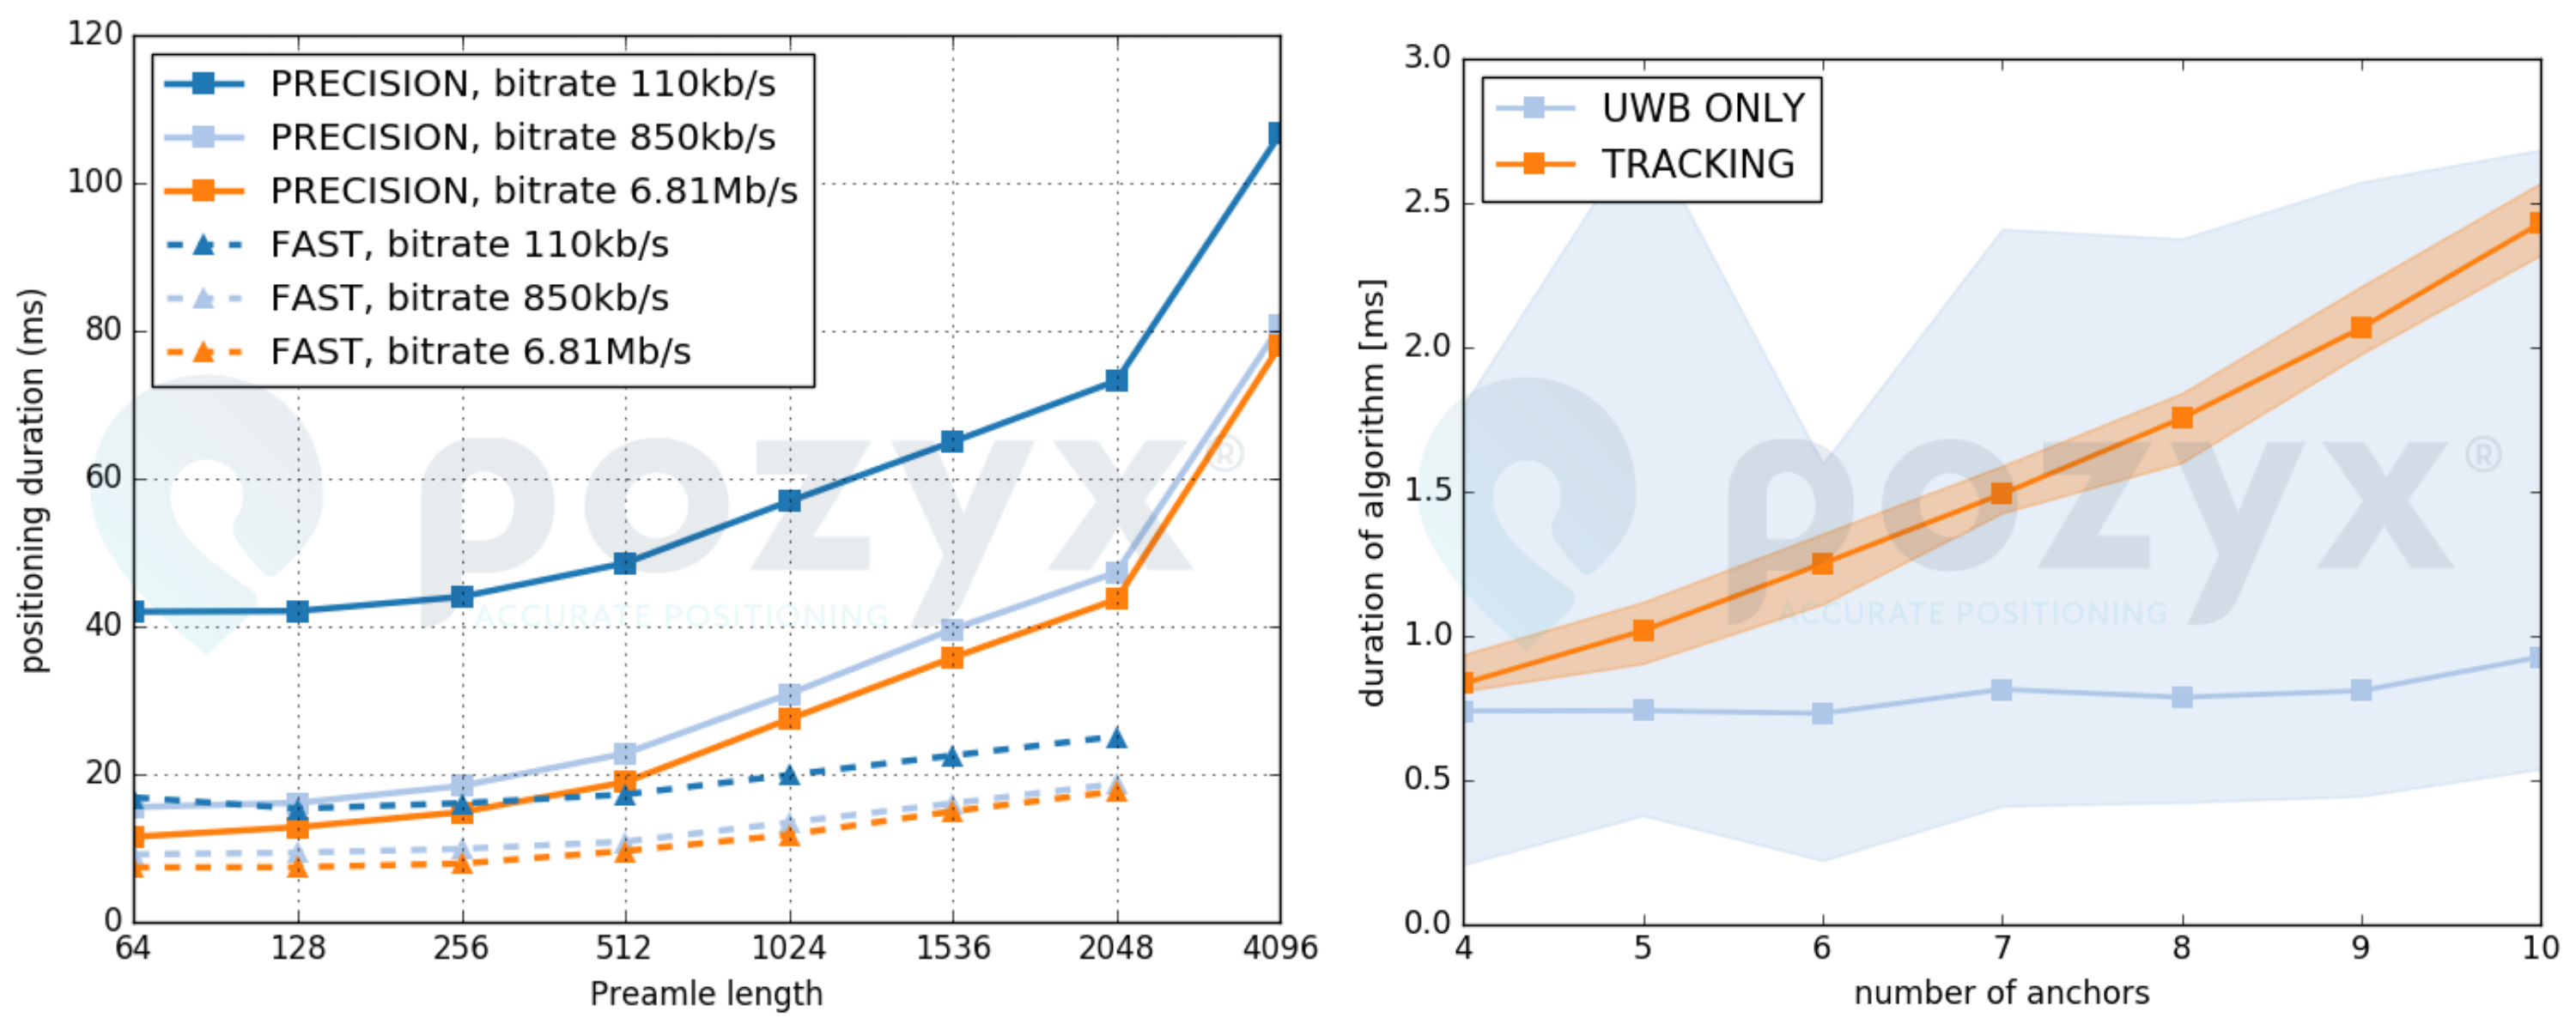
\includegraphics[scale=0.17]{durata_pozyx}
	 			\caption{\textbf{Figura 7:} Durata del \textit{doPositioning} e \textit{doRanging} tratte dal sito Pozyx}\label{Fdur_pozyx}
			\end{figure}

		\end{subsubsection}

		\begin{subsubsection}{Update rate delle istruzioni d'interesse}

			Nella sezione precedente, i valori di frequenza ottenuti riguardavano solo il \textit{doPositioning} e il \textit{doRanging} senza però tener conto del tempo accumulato durante la stampa su seriale. Inoltre, per i nostri obiettivi, non basta stampare le coordinate, eseguendo quindi il \textit{doPositioning} dei due 					tag, ma occorre sapere anche le distanze dalle singole ancore. Questo, come precedente spiegato, è reso possibile dall’istruzione \textit{getDeviceRangeInfo}.
			Qui di seguito verranno illustrati gli esperimenti condotti per ricavare gli update rate delle istruzioni sopra descritte. Riguardo a queste ultime, abbiamo differenziato la frequenza di lavoro ottenuta includendo o trascurando la durata della stampa attraverso la funzione \textit{print()}. Inoltre, l’analisi è stata 						condotta sia in presenza di un singolo tag che di due device collegati ad Arduino.

			In \textbf{\tablename~\ref{Tfreqop}} sono riportate le frequenze di lavoro relative alle istruzioni eseguite (A, B, C, D) in 3 prove successive. Durante tutto questo periodo di tempo, tag e ancore, hanno occupato le stesse posizioni in ambiente indoor, contenenti tipici oggetti di disturbo elettromagnetico utilizzati 			in un laboratorio. 

			\begin{table}[h]
				\centering
				\begin{tabular}{|l|c|c|c|c|c|c|c|c|}
					\hline
					\multicolumn{9}{|c|}{}\\
					\multicolumn{9}{|c|}{\textbf{\Large Frequenza di lavoro [Hz]}}\\
					\multicolumn{9}{|c|}{}\\
					\hline
					\multirow{2}{*}{}&		\multicolumn{2}{|c|}{Prova 1}&					\multicolumn{2}{|c|}{Prova 2}&					\multicolumn{2}{|c|}{Prova 3}&				\multicolumn{2}{|c|}{Medie}\\
					\cline{2-9}
					 &									1 TAG&					2 TAG&								1 TAG&					2 TAG&								1 TAG&					2 TAG&							1 TAG&					2 TAG\\
					\hline
					{\textbf{A}}&				110$\pm$10&		54$\pm$3&						110$\pm$10&		57$\pm$4&						100$\pm$7&			51$\pm$3& 					104$\pm$8&			52$\pm$3\\	
					\hline	
					{\textbf{B}}&	 			83$\pm$6&			41$\pm$2&						83$\pm$6&			42$\pm$2& 						76$\pm$5&			39$\pm$2&					78$\pm$5	&			40$\pm$2\\	
					\hline	
					{\textbf{C}}&	 			89$\pm$6&			43$\pm$3&						88$\pm$6&			45$\pm$3& 						78$\pm$5&			40$\pm$2& 					81$\pm$6&			41$\pm$2\\	
					\hline	
					{\textbf{D}}&				45$\pm$10&			34$\pm$0&						67$\pm$1&			22$\pm$1& 						45$\pm$6&			21$\pm$1& 					47$\pm$2&			26$\pm$1\\	
					\hline				
				\end{tabular}
				\caption{\textbf{Tabella 4: } Frequenza di lavoro al variare delle operazioni eseguite: A) \textbf{doPositioning} con printing di coordinate; B) \textbf{doPositioning} e \textbf{getDeviceRangeInfo} con printing di coordinate e range; C) \textbf{doPositioning} e \textbf{getDeviceRangeInfo} con printing del 																		range; D) \textbf{doRanging} con printing di range\label{Tfreqop}}
			\end{table}
			Per ogni prova riportata si nota facilmente che la frequenza raggiunta utilizzando un tag è circa il doppio di quella con due tag. Come ci si aspettava, stampando più valori, la frequenza di lavoro diminuisce. Infatti, rispetto all’analisi condotta nella sezione precedente, le frequenze risultano più basse.\\
			Considerando che l'algoritmo di positioning necessita preliminearmente della misura di quattro distanze, appare sorprendente il risultato ottenuto nel caso del \textit{doRanging}. In tale esperimento vengono richieste le quattro distanze dalle ancore, ma la frequenza di lavoro calcolata risulta inferiore rispetto 					agli altri casi.

			La riga di questa tabella che a noi interesserà maggiormente è quella relativa alla lettera \textbf{B}. Si considerano le operazioni di \textit{doPositioning} e \textit{getDeviceRangeInfo} con le corrispondenti stampe. Prendendo in considerazione i valori di frequenza media, calcolati per ogni singola prova, il 						massimo ammota a $42Hz$.

		\end{subsubsection}


		\begin{subsubsection}{SerialPort}
			\hypertarget{SS2}{Come} già anticipato, Arduino comunica con il pc attraverso la porta USB. Per conseguire il nostro obiettivo, ovvero raggiungere il massimo update rate, l'analisi si è concentrata su quali istruzioni dello sketch di Arduino potessero rallentarne l’esecuzione.\\ Nel \textit{void loop()} di 								Arduino sono essenzialmente tre le istruzioni che hanno un tempo di esecuzione rilevante: \textit{doPositioning}; \textit{getDeviceRangeInfo} e la stampa a video dei valori. La valutazione del tempo impiegato dal \textit{doPositioning} e \textit{getDeviceRangeInfo} ad aggiornare le misure è stata 									trattata precedentemente.\\ Questa sezione valuta la durata temporale dell’istruzione di stampa e offre una possibile alternativa alla soluzione standard. In dettaglio, è stata scaricata e installata la libreria <SerialPort.h>$^{{\cite{cit17}}}$.\\In una fase preliminare, é stato realizzato un semplice sketch per la 					stampa di una stringa contenente lo stesso numero e tipo di valori restituiti dal sistema Pozyx.  Per ogni tag, tale stringa contiene tre \textit{int32\_t} (valore numerico intero con segno, dimensione di $4bytes$), relativi alle coordinate e 						quattro \textit{uint32\_t} (valore numerico intero senza 						segno, dimensione di $4bytes$), relativi alle distanze dalle ancore. Lo sketch è stato testato due volte: prima utilizzando la seriale standard di Arduino e successivamente la SerialPort. 
			Eseguendo dunque, una volta l’istruzione \textit{Serial.write} e dopo \textit{NewSerial.write}, si ottengono i risultati illustrati in \textbf{\figurename~\ref{Fconfronto}}. I test sono stati ottenuti utilizzando i parametri UWB segnalati dall'azienda come migliori in termini di frequenza (\textbf{channel} = 5; 							\textbf{bitrate} = 6.81 Mbit/s; \textbf{plen} = 64; \textbf{prf} = 64).

			\begin{figure}[h]
				\centering
				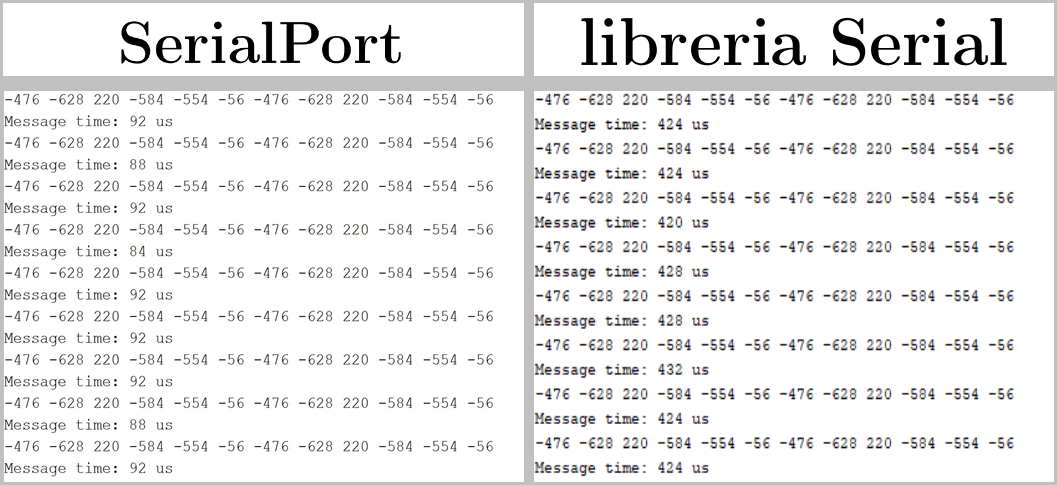
\includegraphics[scale=0.45]{conf_serial_newSerial}
	 			\caption{\textbf{Figura 8:} Esperimenti preliminari di valutazione della nuova libreria rispetto alla standard}\label{Fconfronto}
			\end{figure}

			Per la stampa dei valori desiderati, è stata utilizzata l’istruzione \textit{write()} e non \textit{print()}. Questo è dovuto al fatto che la seconda delle due effettua una conversione del valore numerico in carattere ASCII, ritardando la stampa e diminuendo di conseguenza la frequenza di lavoro. Un'ulteriore ragione 				di questa scelta è che il comando \textit{write()} stampa una stringa in codice binario. Questo risulterà utile nel momento in cui si volessero collegare i tag ad un autopilota, già abilitato alla lettura di valori in tale formato.\\ 
			Dunque, questa prima analisi lasciava intendere che l'update rate sarebbe aumentata, dato che le durate temporali ottenute, utilizzando la libreria alternativa, risultavano notevolmente inferiori. In realtà, valutando successivamente la frequenza di lavoro dell’intero loop con NewSerial.write, il recupero 								rispetto alla seriale standard non sembra essere effettivo. Infatti, come si evince dai valori riportati in \textbf{\tablename~\ref{Tserialport}}, l'update rate dei dati relativi a due tag derivanti dal normale utilizzo delle antenne, oscilla intorno a $40 Hz$, frequenza raggiunta anche dalla seriale standard, come 						riassuntivamente si può vedere in \textbf{\tablename~\ref{Tserialportconfronto}}. Ciò potrebbe essere dovuto al fatto che nell'esecuzione, la conversione in carattere ASCII occupi un tempo rilevante.
			Nonostante i risultati non mostrino differenze sostanziali, tutti gli esperimenti descritti successivamente sono stati condotti utilizzando la SerialPort. Una cosa importante da tenere presente, è che è stata utilizzata tale libreria impostando la dimensione del Buffer della seriale pari a $64 bytes$, scelta consona 						rispetto al pacchetto di dati che necessitiamo stampare ($60 bytes$). Se volessimo stampare più di $64 bytes$, bisognerebbe aumentare la dimensione del Buffer per evitare che l'invio del pacchetto su seriale richieda un tempo superiore al necessario.				

			\begin{table}[h]
				\centering
				\begin{tabular}{|c|c|c|}
					\hline
					\multicolumn{3}{|c|}{}\\
					\multicolumn{3}{|c|}{\textbf{\Large Frequenza di lavoro [Hz]}}\\
					\multicolumn{3}{|c|}{\textbf{\Large SerialPort}}\\
					\multicolumn{3}{|c|}{}\\
					\hline
					&								1 Tag&						2 Tag\\
					\hline
					Prova 1&					78$\pm$6&				38$\pm$2\\
					\hline
					Prova 2&					74$\pm$4&				40$\pm$3\\
					\hline
					Prova 3&					76$\pm$4&				41$\pm$2\\
					\hline
					Prova 4&					75$\pm$5&				39$\pm$2\\
					\hline
					Prova 5&					80$\pm$6&				39$\pm$2\\
					\hline
					Prova 6&					78$\pm$6&				40$\pm$2\\
					\hline 				
				\end{tabular}
				\caption{\textbf{Tabella 5: } Esperimenti condotti sulla libreria SerialPort.\label{Tserialport}}
		\end{table}

		\begin{table}[h]
			\centering
			\begin{tabular}{|c|c|c|c|c|}
						\hline
						\multicolumn{5}{|c|}{}\\
						\multicolumn{5}{|c|}{\textbf{\Large Frequenza di lavoro [Hz]}}\\
						\multicolumn{5}{|c|}{\textbf{\Large confronto librerie Serial}}\\
						\multicolumn{5}{|c|}{}\\
						\hline
						&																															\multicolumn{2}{|c|}{SerialPort}&														\multicolumn{2}{|c|}{Seriale Arduino}\\
						\hline
						\multirow{2}{*}{DoPositioning + getDeviceRangeInfo}&				1Tag&							2 Tag&															1Tag&							2 Tag\\
						\cline{2-5}
						&																																77$\pm$6&					40$\pm$2&													78$\pm$5&					40$\pm$2\\
						\hline
			\end{tabular}
			\caption{\textbf{Tabella 6: } Confronto delle medie calcolate dagli esperimenti condotti attraverso l'utilizzo delle due librerie seriali, atampando su seriale sia le coordinate che le distanze.\label{Tserialportconfronto}}
		\end{table}

		\end{subsubsection}
		\newpage

		\begin{subsubsection}{Scelta configurazione ottimale parametri UWB}

			\hypertarget{SS1}{In} questa sezione è stata testata la configurazione di parametri UWB (\hyperlink{S3}{\textbf{sezione Parametri}} per ulteriori dettagli) ottimale ai fini di ottenere la massima frequenza di update. Tra gli sketch, è presente uno denominato “UWB configurator” il quale consente in modo 						interattivo di selezionare dal monitor seriale sia le ancore che il tag e impostarne i parametri UWB desiderati. In \textbf{\figurename~\ref{FUWBconfigurator}} è riportata la finestra con cui l'utente si interfaccerà per effettuare tali modifiche. Ogni dispositivo memorizzerà l’insieme dei parametri settati nella sua 					memoria flash e manterrà tale configurazione fino a quando non verrà nuovamente impostata. Per il momento tra le possibili variabili UWB non viene preso in considerazione il gain, in quanto su di esso è stato condotto un apposito esperimento riportato di seguito. Le configurazioni possibili sono tantissime, ma 			ai fini di questo lavoro solo alcune di esse vengono prese in considerazione.\\
			\begin{figure}[H]
				\centering
				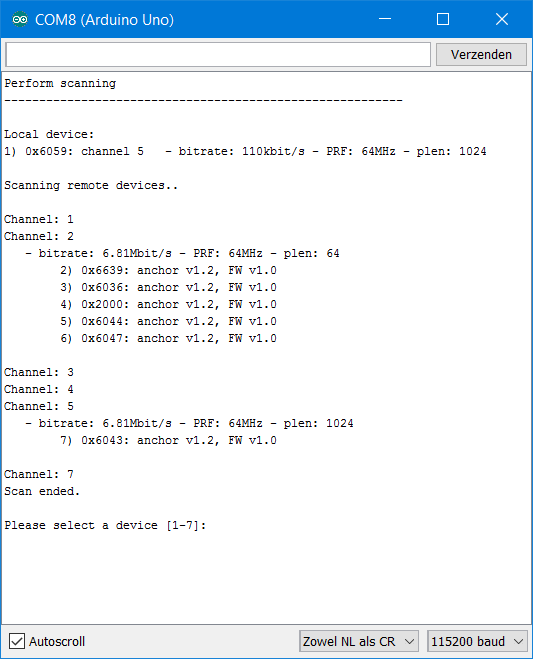
\includegraphics[scale=0.6]{FUWBconfigurator}
	 			\caption{\textbf{Figura 9:} sketch per variare i parametri\label{FUWBconfigurator}}
			\end{figure}
			Punto di partenza è stata la documentazione Pozyx, nel dettaglio si fa riferimento a quanto riportato in \textbf{\figurename~\ref{Fdur_pos}} che riassume i risultati ottenuti dall'azienda. Seguendo questa tabella innanzitutto si è impostato il protocollo di ranging a \textit{fast}.

			La prima analisi effettuata ha investigato la dipendenza dell'update rate dal \textbf{bitrate} fissando gli altri parametri UWB pari a: \textbf{channel} = $5$; \textbf{plen} = $64$; \textbf{prf} = $64 MHz$. Da notare come i test da noi effettuati, però, fossero su due tag in parallelo ad Arduino. Ciò implica un						dimezzamento, circa, della frequenza di lavoro rispetto all'utilizzo di un solo tag. I risultati dei nostri test sono riportati in \textbf{\figurename~\ref{FFreqBit}}. 

			\begin{figure}[H]
				\centering
				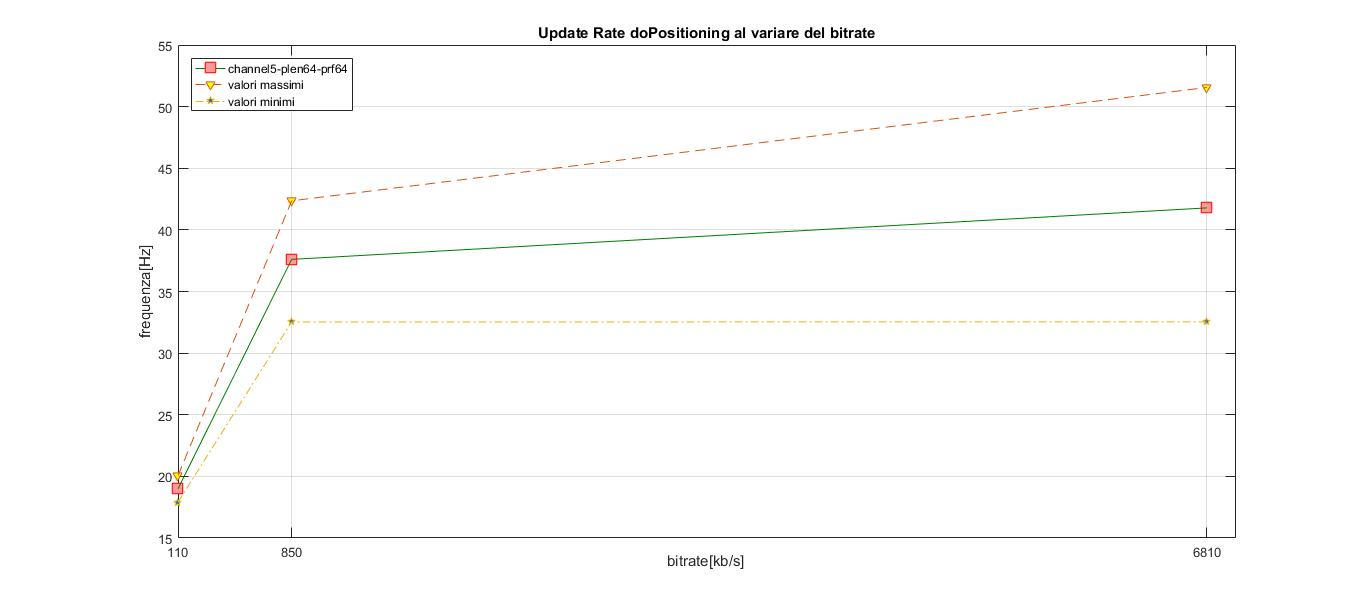
\includegraphics[scale=0.3]{FreqBit} 	
				\caption{\textbf{Figura 10:} Esperimenti al variare del \textbf{bitrate}\label{FFreqBit}}		
			\end{figure}
			\begin{table}[H]
						\centering
						\begin{tabular}{|c|c|c|c|}
							\hline
							\multicolumn{4}{|c|}{}\\
							\multicolumn{4}{|c|}{\textbf{\Large Parametri}}\\
							\multicolumn{4}{|c|}{}\\
							\hline
							Channel = 5,& \multicolumn{3}{|c|}{Bitrate [kbit/s]}\\
			\cline{2-4}
							 prf = 64 MHz, plen =  64& 110& 850& 6810\\
			\hline
			Frequenza [Hz] & 19$\pm$0.4& 37.67$\pm$1.2& 41.78$\pm$2.5\\
			\hline
							\end{tabular}
			\end{table}
			È quindi evidente, come ci si aspettava ed a conferma dalla documentazione, che la dipendenza dal \textbf{bitrate} esista e ci sia un andamento monotono crescente rispetto ad esso. Si nota, inoltre, un maggiore incremento di frequenza nel passaggio da $110kbit/s$ a $850kbit/s$ rispetto a quello da $850kbit/				s$	a $6.81Mbit/s$.\\
			Trovato il valore ottimo per questo parametro, pari a $6.81Mbit/s$, è stato quindi condotto un ulteriore set di esperimenti. Esso è stato volto a verificare, a parità di \textbf{channel} e \textbf{prf}, con \textbf{bitrate} = $6.81Mbit/s$,  la variazione della frequenza rispetto al \textbf{plen}. I dati relativi ai test 					condotti sono riportati in \textbf{\figurename~ \ref{FFreqPlen}}.

			\begin{figure}[H]
				\centering
				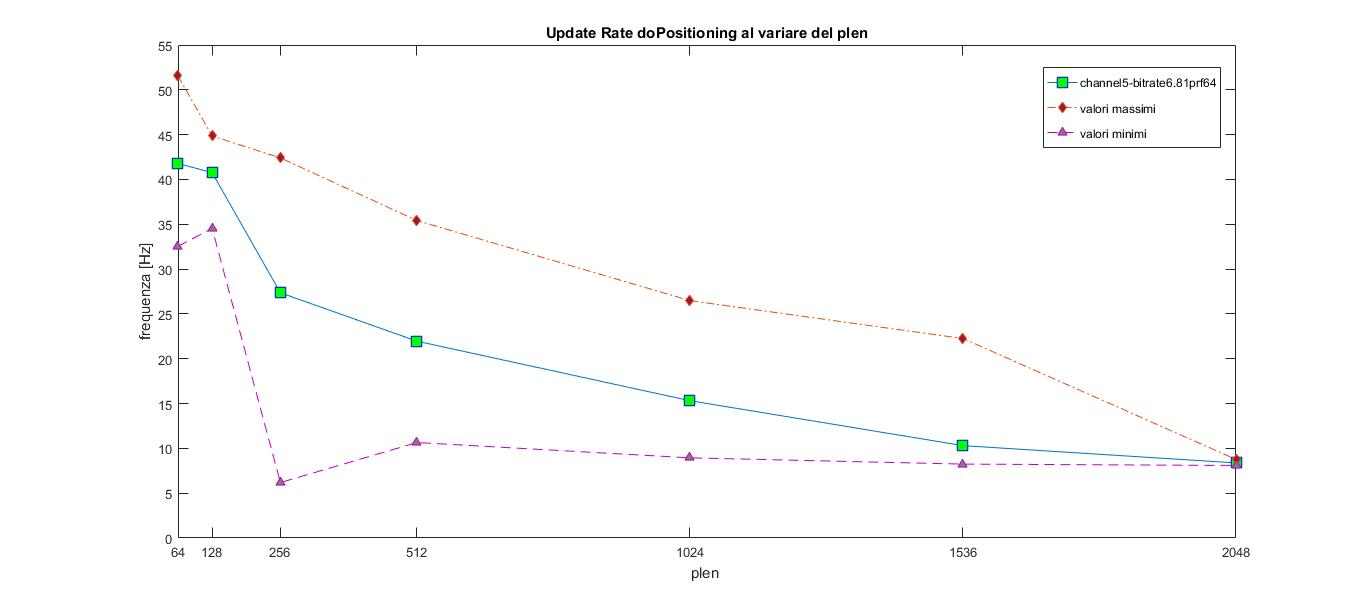
\includegraphics[scale=0.3]{FreqPlen}
				\caption{\textbf{Figura 11:} Esperimenti al variare del \textbf{plen}\label{FFreqPlen}}
			\end{figure}
			\begin{table}[H]
						\centering
\resizebox*{1.0\textwidth}{!}{
			\begin{tabular}{|c|c|c|c|c|c|c|c|}
						\hline
						\multicolumn{8}{|c|}{}\\
						\multicolumn{8}{|c|}{\textbf{\Large Parametri}}\\
						\multicolumn{8}{|c|}{}\\
						\hline
							Channel = 5,& \multicolumn{7}{|c|}{plen}\\
						\cline{2-8}
							 prf = 64 MHz, bitrate =  6810 kbit/s& 64& 128& 256& 512& 1024& 1536& 2018\\
							\hline
						Frequenza [Hz] & 41.78$\pm$2.4& 40.76$\pm$1.6& 27.36$\pm$13& 21.97$\pm$10.7& 15.31$\pm$7.46& 10.30$\pm$4.0& 8.37$\pm$0.1\\
						\hline
			\end{tabular}
}
			\end{table}

			Anche qui l'andamento della frequenza rispecchia quelle che erano le attese: all'aumentare del \textbf{plen} la frequenza decresce con un andamento monotono. L'unica ulteriore osservazione è che la differenza di frequenza con \textbf{plen} pari a $64$ e a $128$ è molto meno significativa che negli 								altri casi.\\

			A questo punto, l'ultima variazione che è stata investigata è quella relativa alla variazione del canale. Questo test è stato effettuato a \textbf{bitrate}, \textbf{prf} e \textbf{plen} fissati. I risultati sono riportati in \textbf{\figurename~\ref{FFreqChan}}.
			Rispetto ai casi precedenti, non è possibile trarre una conclusione univoca. Infatti, anche se il \textbf{channel} di default (\textbf{channel} = 5) sembrerebbe essere leggermente migliore in termini di frequenza di lavoro, la differenza rispetto agli altri è talmente piccola che non è possibile generalizzare che esso 				sia il canale migliore. In base alle condizioni ambientali in cui ci si trova, quindi, converrebbe effettuare un test preliminare per determinare il più adatto valore per questo parametro.
			\begin{figure}[H]
				\centering
				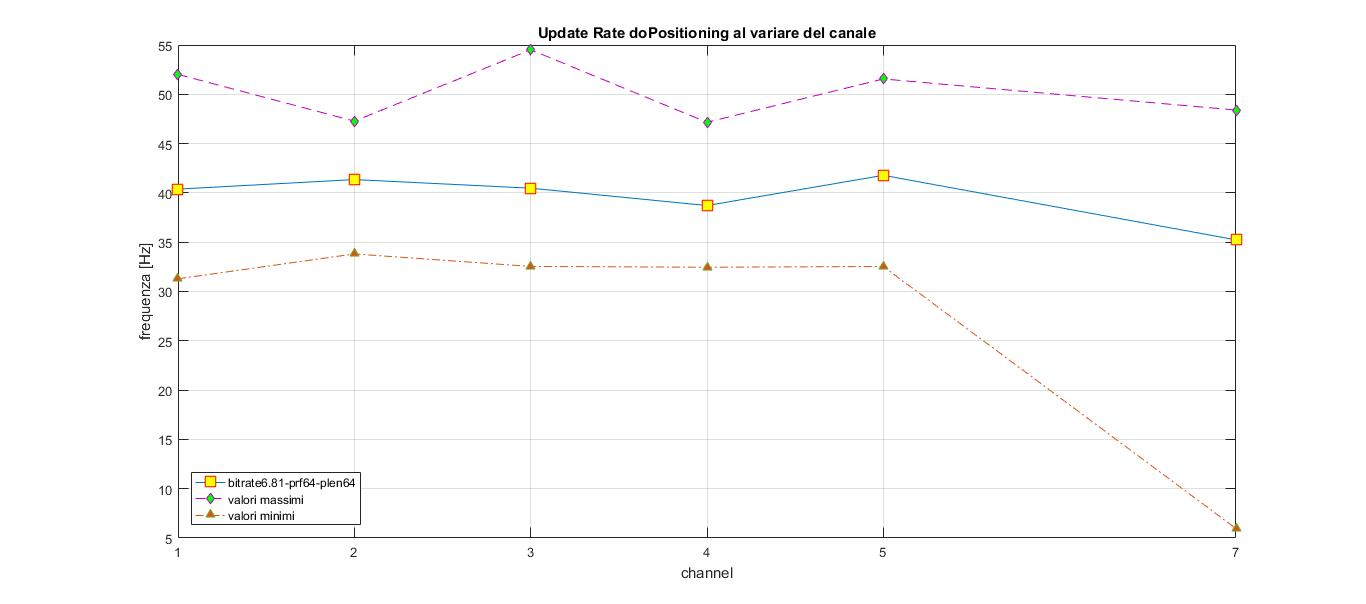
\includegraphics[scale=0.3]{FreqChan}
	 			\caption{\textbf{Figura 12:} Esperimenti al variare del \textbf{channel}\label{FFreqChan}}
			\end{figure}
			\begin{table}[H]
						\centering
\resizebox*{1.0\textwidth}{!}{
			\begin{tabular}{|c|c|c|c|c|c|c|}
						\hline
						\multicolumn{7}{|c|}{}\\
						\multicolumn{7}{|c|}{\textbf{\Large Parametri}}\\
						\multicolumn{7}{|c|}{}\\
						\hline
						Bitrate =  6810 kbit/s	,& \multicolumn{6}{|c|}{plen}\\
						\cline{2-7}
						prf = 64 MHz, plen = 64 & 1& 2& 3& 4& 5& 7\\
						\hline
						Frequenza [Hz] & 40.38$\pm$2.9& 41.35$\pm$1.9& 40.48$\pm$2.7& 38.72$\pm$2.1& 41.78$\pm$2.5& 35.24$\pm$7.6\\
						\hline
				\end{tabular}
}
			\end{table}

		\end{subsubsection}
		
		\begin{subsubsection}{Gain}

			Nel caso in cui si volesse utilizzare il sistema Pozyx in aree di lavoro più ampie, dalla documentazione si evince come risulti necessario un aumento del gain. Fino ad ora lo sketch di configurazione dei parametri UWB impostava automaticamente tale parametro al valore di default ($11.5$). Nel seguente 								esperimento, è stato, invece, valutato se e quanto l’aumentare del guadagno influenzi la frequenza di lavoro. Le condizioni di lavoro sono le stesse degli altri esperimenti indoor, con due tag collegati parallelamente. In particolare un tag è collegato diretteamente su Arduino, mentre l'altro è collegato ad una 						distanza di circa $40cm$ tramite collegamenti con dei jumper solo nei pin precedentemente elencati. In \textbf{\figurename~\ref{EspGain}} è riportata tale configurazione. 
			\begin{figure}[h]
				\centering
				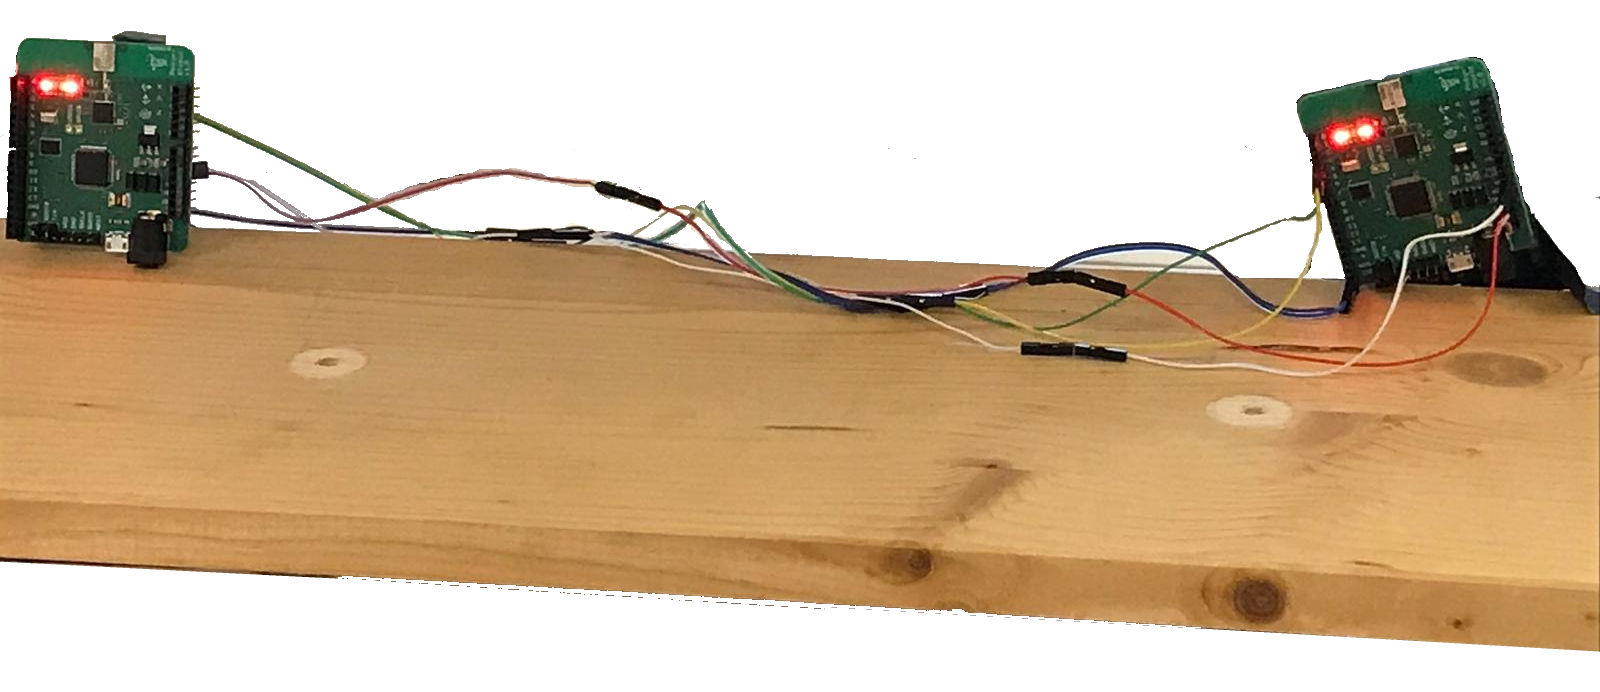
\includegraphics[scale=0.25]{EspGain}
	 			\caption{\textbf{Figura 13:} Configurazione dell'esperimento al variare del \textbf{gain}\label{EspGain}}
			\end{figure}
			Sono stati effettuati due di questi test i cui dati sono riportati in \textbf{\tablename~\ref{TGainF}}. 
			\begin{table}[h]
				\centering
				\footnotesize
				\begin{tabular}{|c|c|c|}
					\hline
					& &\\
					Gain\textsubscript{ [dB]}&	F\textsubscript{ [Hz]} esperimento 1 & F\textsubscript{ [Hz]} esperimento 2\\
					& &\\
					\hline
					11.5&			26&		37\\ 
					\hline
					15&				27&		39\\ 
					\hline
					20&				31&		40\\ 
					\hline
					25&				37&		39\\ 
					\hline
					30&				38&		39\\ 
					\hline
					33&				38&		36\\ 
					\hline
				\end{tabular}
				\caption{\textbf{Tabella 7: } Studio della frequenza al variare del Gain\label{TGainF}}
			\end{table}
			Dai dati riportati in tabella relativi ad un primo esperimento, sembrava sussistere una dipendenza della frequenza dal gain. Questa è stata però smentita dal secondo esperimento, che ha prodotto dei risultati praticamente stazionari rispetto alla variabile. I cambiamenti sembrano molto più dipendenti dalle variazioni 					delle condizioni ambientali piuttosto che al parametro in analisi. Si evince, quindi, una già nota aleatoreità della frequenza di lavoro, ma altresì una indipendenza della stessa dalla variazione del gain.

		\end{subsubsection}
		\end{subsection}

		\begin{subsection}{Verifica Precisione ed Accuratezza delle misure}

			Il test successivo è stato condotto per verificare la precisione delle misure in uscita dall’algoritmo di positioning e di ranging. Parallelamente, è stato condotta anche un’analisi sull’accuratezza. Da notare, però, come l’accuratezza delle misure sia stata valutata solo sulle distanze. Questo perchè, avendo a 							disposizione un metro laser, è stato possibile misurare le distanze tra i tag e le varie antenne, ma non delle coordinate.
			L’esperimento è stato condotto sotto le stesse condizioni di lavoro descritte in precedenza, con i due tag posizionati l’uno sull’altro e connessi ad Arduino. Per maggiore chiarezza si faccia riferimento a  \textbf{\figurename~\ref{FEspPrecis}}. Di questo esperimento sono state condotte tre prove.
			
			\begin{figure}[h]
				\centering
				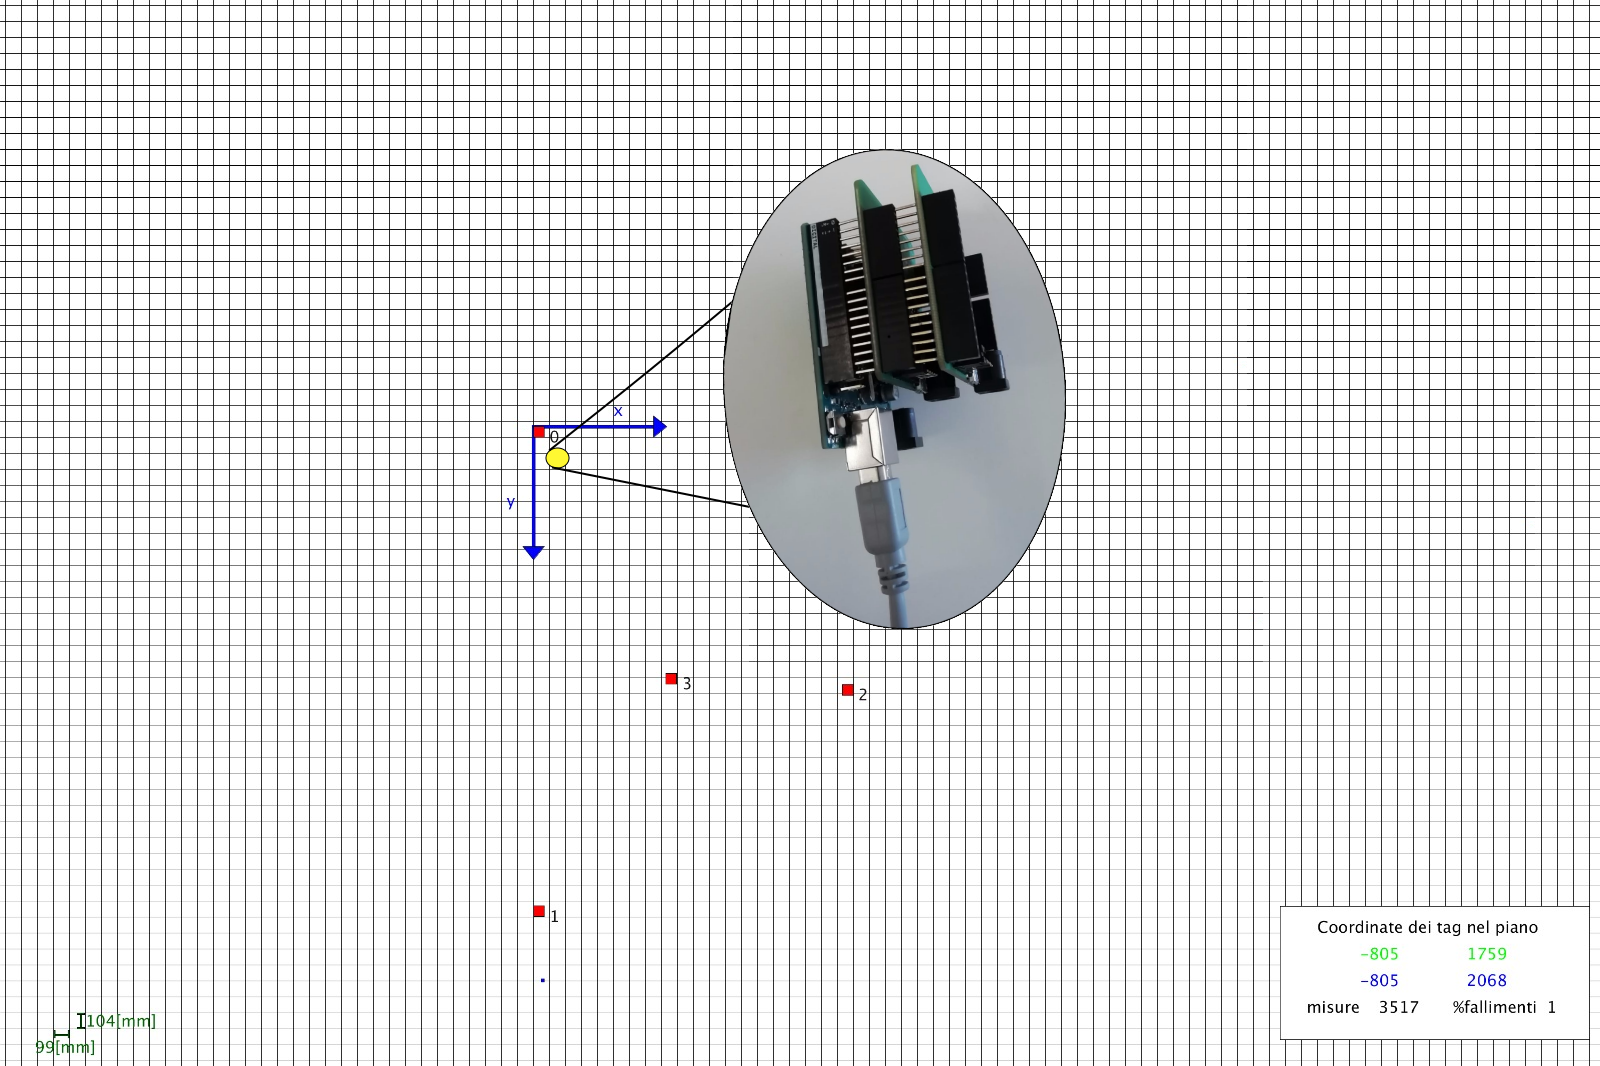
\includegraphics[scale=0.55]{EspPrecis}
	 			\caption{\textbf{Figura 14:} Descrizione dell'esperimento\label{FEspPrecis}}
			\end{figure}
			I dati sono stati graficati tramite l’utilizzo dello skecth su Processing 3 per avere un riscontro in tempo reale dell’esito dell’esperimento. Il risultato dei tre esperimenti viene riportato in \textbf{\figurename~\ref{FEspPrecis1}}.
			In post-processing è stata condotta l’analisi sui dati salvati. Vengono calcolate media e deviazione standard per valutare la precisione; è possibile esaminare l’accuratezza del ranging confrontando i dati con le distanze reali dalle ancore. Tali risultati sono riportati nelle \textbf{\tablename~\ref{EspPrecis1}},  						\textbf{\tablename~\ref{EspPrecis2}} che si riferiscono, rispettivamente, al primo ed al secondo tag. 
			\begin{figure}[H]
				\centering
				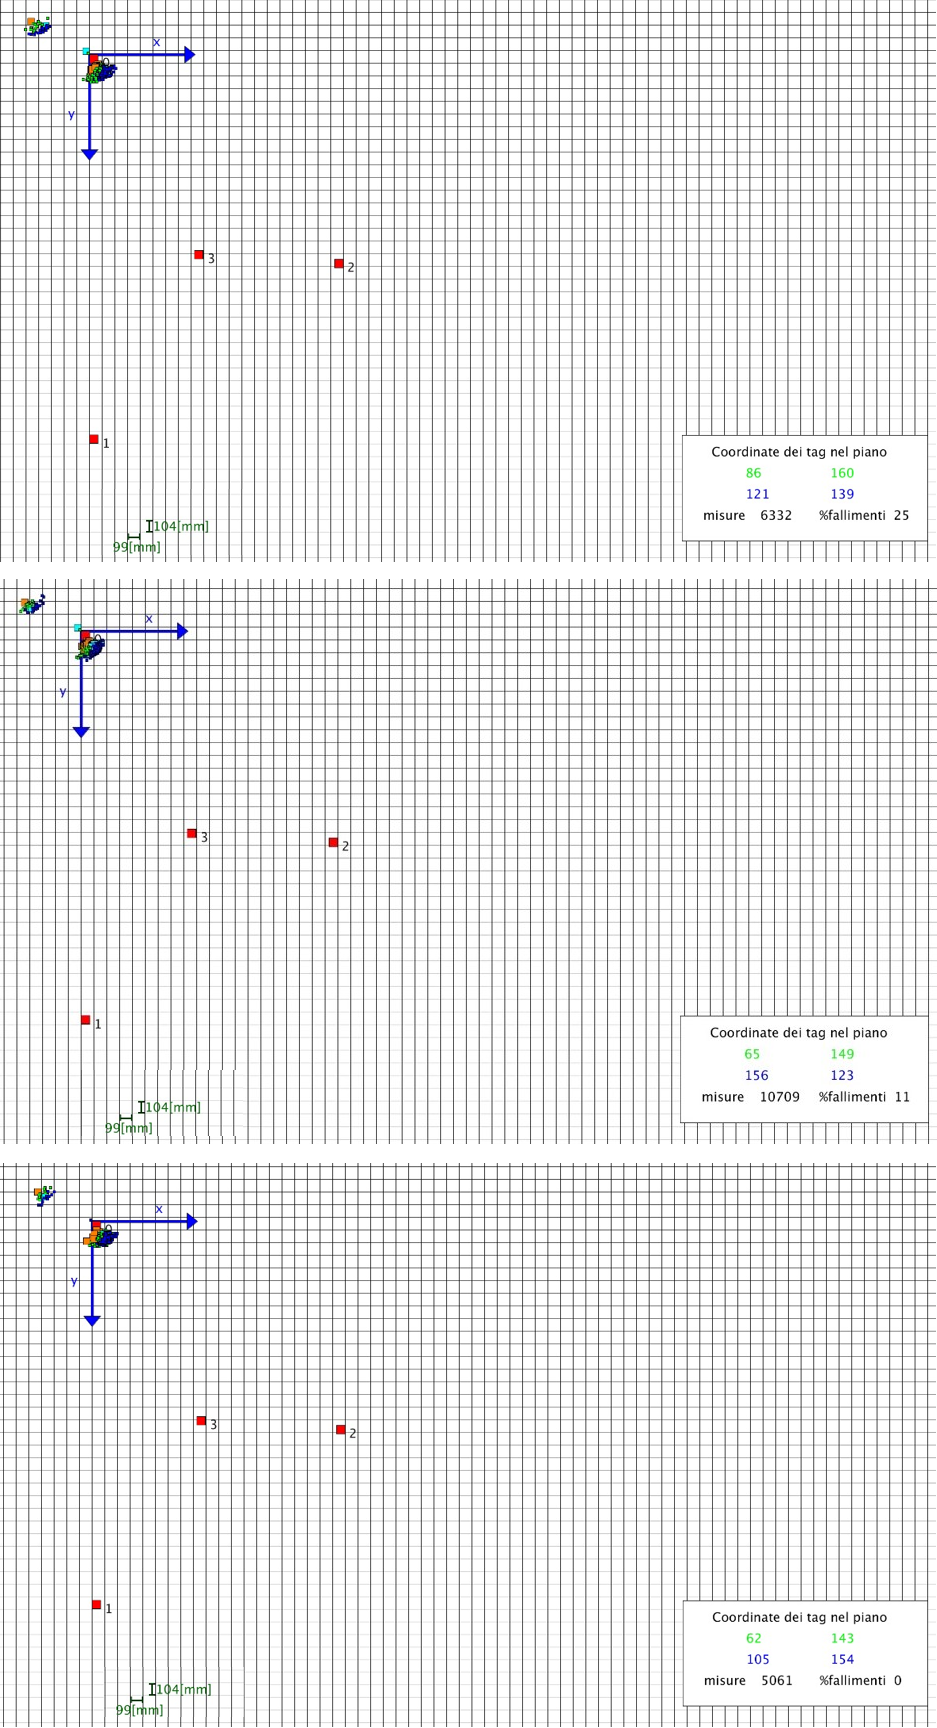
\includegraphics[scale=0.45]{EspPrecis1}
	 			\caption{\textbf{Figura 15:} Processing dei tre esperimenti condotti\label{FEspPrecis1}}
			\end{figure}

			\begin{table}[H]
				\centering
				\begin{tabular}{|c|c|c|c|c|c|}
					\hline
					\multicolumn{6}{|c|}{}\\
					\multicolumn{6}{|c|}{\textbf{\Large Verifica Precisione - Tag 1}}\\
					\multicolumn{6}{|c|}{}\\
					\hline
					\multicolumn{2}{|c|}{}&												Prova 1&							Prova 2&						Prova 3&					Misure reali\\
					\hline
					\multirow{3}{*}{Coordinate [mm]}&			x&					55.4$\pm$35&					73$\pm$13&					64.2$\pm$26&			-\\
					\cline{2-6}
					&																y&					110$\pm$66&					147$\pm$15&				129.1$\pm$49&		-\\
					\cline{2-6}
					&																z&					77.7$\pm$35&					91.6$\pm$36&				77.7$\pm$35&			-\\
					\hline
					\multicolumn{2}{|c|}{Distanza 0}&								63$\pm$27&						62$\pm$28&					64$\pm$28&				230\\
					\hline
					\multicolumn{2}{|c|}{Distanza 1}&								2672.5$\pm$28&				2672$\pm$28&				2674.1$\pm$31&		2698\\
					\hline
					\multicolumn{2}{|c|}{Distanza 2}&								2317.3$\pm$35&				2322$\pm$20&				2322$\pm$18&			2420\\
					\hline
					\multicolumn{2}{|c|}{Distanza 3}&								1810.2$\pm$22&				1810$\pm$22&				1811$\pm$22&			1712\\
					\hline
				\end{tabular}
				\caption{\textbf{Tabella 8: } Risultati delle tre prove sulla precisione del tag1. NOTA: la Distanza i-esima (con i = 0,1,2,3), indica la distanza tra il tag e la corrispettiva ancora, numerata a partire da 0.\label{EspPrecis1}}
			\end{table}

			\begin{table}[H]
				\centering
				\begin{tabular}{|l|c|c|c|c|c|}
					\hline
					\multicolumn{6}{|c|}{}\\
					\multicolumn{6}{|c|}{\textbf{\Large Verifica Precisione - Tag 2}}\\
					\multicolumn{6}{|c|}{}\\
					\hline
					\multicolumn{2}{|c|}{}&												Prova 1&							Prova 2&						Prova 3&					Misure reali\\
					\hline
					\multirow{3}{*}{Coordinate [mm]}&			x&					81.8$\pm$50&					109.6$\pm$18&			97.15$\pm$38&		-\\
					\cline{2-6}
					&																y&					122.6$\pm$73&				161.4$\pm$15&			140.8$\pm$53&		-\\
					\cline{2-6}
					&																z&					118.7$\pm$83&				154.13$\pm$37&			132.2$\pm$52&		-\\
					\hline
					\multicolumn{2}{|c|}{Distanza 0}&								159$\pm$22&					159.4$\pm$23&			159$\pm$23&			230\\
					\hline
					\multicolumn{2}{|c|}{Distanza 1}&								2687.6$\pm$24&				2690.6$\pm$25&			2694$\pm$26&			2698\\
					\hline
					\multicolumn{2}{|c|}{Distanza 2}&								2294.6$\pm$21&				2298.7$\pm$21&			2297$\pm$22&			2420\\
					\hline
					\multicolumn{2}{|c|}{Distanza 3}&								1757.7$\pm$29&				1758$\pm$26&			1760$\pm$25&				1712\\
					\hline
				\end{tabular}
				\caption{\textbf{Tabella 9: } Risultati delle tre prove sulla precisione del tag2. NOTA: la Distanza i-esima (con i = 0,1,2,3), indica la distanza tra il tag e la corrispettiva ancora, numerata a partire da 0.\label{EspPrecis2}}
			\end{table}

			Da questi dati si evince un alto grado di precisione, essendo la deviazione massima riscontrata pari a $83mm$. Il fatto stesso che le tre prove diano risultati di posizione molto simili tra loro, supporta quanto apperna espresso. Inoltre, dalle stesse tabelle, si può evincere un alto grado di accuratezza, 									comparabile con i $10cm$ dichiarati dall’azienda. L’unica nota che va fatta è sulla distanza tra il \textit{tag 1} e l’\textit{ancora 0}. In questo caso, infatti, la differenza rispetto ai valori reali è risultata più marcata. Questa piccola discrepanza è, però, imputabile alla configurazione scelta per l'esperimento. Qui, i 					due tag sono posizionati di fronte l’ancora suddetta; il \textit{tag 2}, quindi, si interpone tra il \textit{tag 1} e l’\textit{ancora 0}, risultando esso stesso una fonte di disturbo alla loro comunicazione. 

		\begin{subsubsection}{Gain}

			Come  già descritto nella \hyperlink{SS5}{\textbf{sottosezione Come funziona UWB}}, il gain determina la potenza del segnale trasmesso, la quale influenza la frequenza degli impulsi trasmessi e di conseguenza l'accuratezza del sistema. Assodato il concetto che un aumento del gain comporti una diminuzione					dell'accuratezza delle misure, in questa sezione viene, quindi, valutata la dipendenza della precisione da questo parametro. I test sono stati condotti fino al raggiungimento di un numero di campioni pari a 2000. Nella \textbf{\tablename~\ref{TGainP}} vengono riportate le medie relative alle misure 									delle coordinate.  Dunque non sembra possibile definire una correlazione tra la precisione ed il guadagno. Infatti la deviazione standard risulta sostanzialmente invariata e l'escursione tra le varie misure delle coordinate risulta essere minima. 

		\begin{table}[h]
					\centering
					\footnotesize
					\begin{tabular}{|c|c|c|c|c|}
						\hline
						&&&&\\
						Gain\textsubscript{ [db]}&		X\textsubscript{tag\textsubscript{1} [mm]}&	Y\textsubscript{tag\textsubscript{1} [mm]}&		X\textsubscript{tag\textsubscript{2} [mm]}&	Y\textsubscript{tag\textsubscript{2} [mm]}\\
						&&&&\\
						\hline
						11.5&			-174$\pm$41&				2035$\pm$45&									74$\pm$16&												1907$\pm$18\\ 
						\hline
						15&				-157$\pm$16&				2041$\pm$18&									86$\pm$16&												1904$\pm$12\\ 
						\hline
						20&				-125$\pm$48&				2067$\pm$53&									103$\pm$22&											1884$\pm$25\\ 
						\hline
						25&				-90$\pm$55&				2072$\pm$50&									125$\pm$24&											1902$\pm$40\\ 
						\hline
						30&				-104$\pm$50&				2109$\pm$61&									160$\pm$18&											1904$\pm$27\\ 
						\hline
						33&				-96$\pm$31&				2149$\pm$54&									171$\pm$25&											1923$\pm$38\\ 
						\hline
					\end{tabular}
					\caption{\textbf{Tabella 10: } Studio al variare del Gain\label{TGainP}}
		\end{table}
		
		\newpage		
		\end{subsubsection}

		\end{subsection}

		\begin{subsection}{Conclusioni sugli esperimenti indoor}

				Tutti gli esperimenti indoor hanno considerato come primo obiettivo quello di massimizzare la frequenza di aggiornamento delle misure. Per ottenere, infatti, il più elevato update-rate è necessario impostare prima di tutto la frequenza di comunicazione I$^2$C al valore massimo ammissibile, cioè pari a 
				$400KHz$. Inoltre, la configurazione dei parametri UWB riscontrata essere ottimale è la seguente: 
				\begin{itemize}
					\item \textbf{bitrate} =  $6810kbit/s$; 
					\item \textbf{plen} = $64 symbols$;
					\item \textbf{prf} = $64MHz$
				\end{itemize}
				Per quanto riguarda il \textbf{channel}, rifacendosi a quanto riscontrato negli esperimenti indoor, non risulta fondamentale la scelta di tale parametro ai fini degli obiettivi proposti in questo lavoro, per cui è rimasto invariato e pari a 5. Si ricorda che è necessario impostare questo set di parametri in ogni 							device del sistema.\\ Riguardo all’analisi statistica delle misure di ranging e positioning, il sistema Pozyx risulta preciso.  Le misure presentano una deviazione standard inferiore a 8.5 cm, che non sembra essere sostanzialmente influenzata dalle variazioni del gain.

		\end{subsection}

	\end{section}
	\newpage
	
	\begin{section}{Esperimenti outdoor}

		Una volta ottenuta un'ampia caratterizzazione in ambiente indoor il sistema è stato sottoposto ad analisi in ambienti aperti. Tali test avevano due principali prerogative: verificare che le caratteristiche notate fossero rispettate anche all'esterno e valutare approssimativamente un'area di lavoro plausibile per questo 				tipo di dispositivi. Volendo, infatti, utilizzare queste antenne su oggetti in movimento in ampie zone, bisogna poter quantificare quanto vaste essere possano essere, prima di perdere il segnale. A differenza dei test indor, però, l'obiettivo dell'esperimento non è legato direttamente all'update-rate, bensì alle distanze 			massime percorribili prima che la comunicazione non risulti più effettiva. L'investigazione condotta ha preso in analisi in particolare le variazioni dei parametri UWB relativi al \textbf{gain} e al \textbf{bitrate}. 

		\begin{subsection}{Esperimento Ranging}

			Il primo esperimento effettuato ha riguardato solo il calcolo del ranging da due tag in parallelo ad un'unica ancora. In particolare, fissata l'ancora, ci si è allontanati da essa di $5m$ alla volta finchè la comunicazione non è cessata completamente. Tutto ciò è stato ripetuto due volte. In entrambi i casi sono stati 					effettuati tre test, al variare del \textbf{bitrate}. La differenza sostanziale tra i due esperimenti risiede nel \textbf{gain}: nel primo caso è stato settato al valore minimo (11.5) e nel secondo a quello massimo (33). Nell'osservare i dati bisogna tenere in considerazione che, mentre nel primo caso i due tag si 						trovavano posti a una distanza di circa $40cm$ l'un dall'altro, nel secondo erano montati l'uno su l'altro come shield di Arduino. Questo non ha avuto ripercussioni ai fini dell'esperimento. La  \textbf{\figurename~\ref{EspOutRan}} mostra la configurazione adottata in uno dei due esperimenti. 

			\begin{figure}[H]
				\centering
				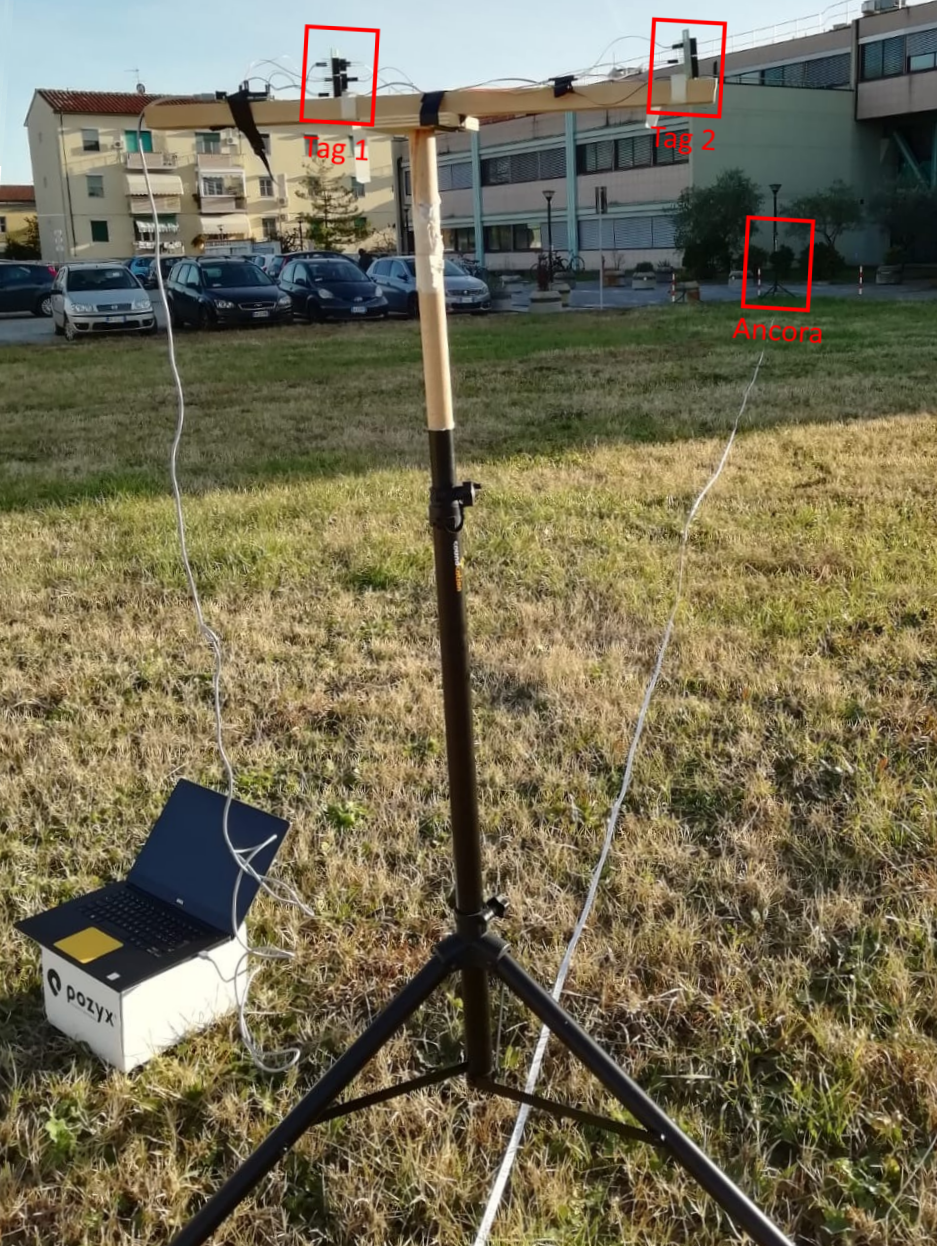
\includegraphics[scale=0.35]{EspOutRan}
	 			\caption{\textbf{Figura 16:} esperimento outdoor di test del ranging\label{EspOutRan}}
			\end{figure}
			Vengono riportati a coppia gli esperimenti svolti ai vari \textit{bitrate}, in modo da verificare come effettivamente l'influenza del gain nel raggiungimento di distanze elevate sia netta. In tutti i casi si nota, infatti, un grande miglioramento in termini di distanza massima raggiunta, fino ad arrivare ad un massimo 					ranging a $60m$ nel caso di \textbf{bitrate}  = $6810kbit/s$. 

			\begin{figure}[H]
				\centering
				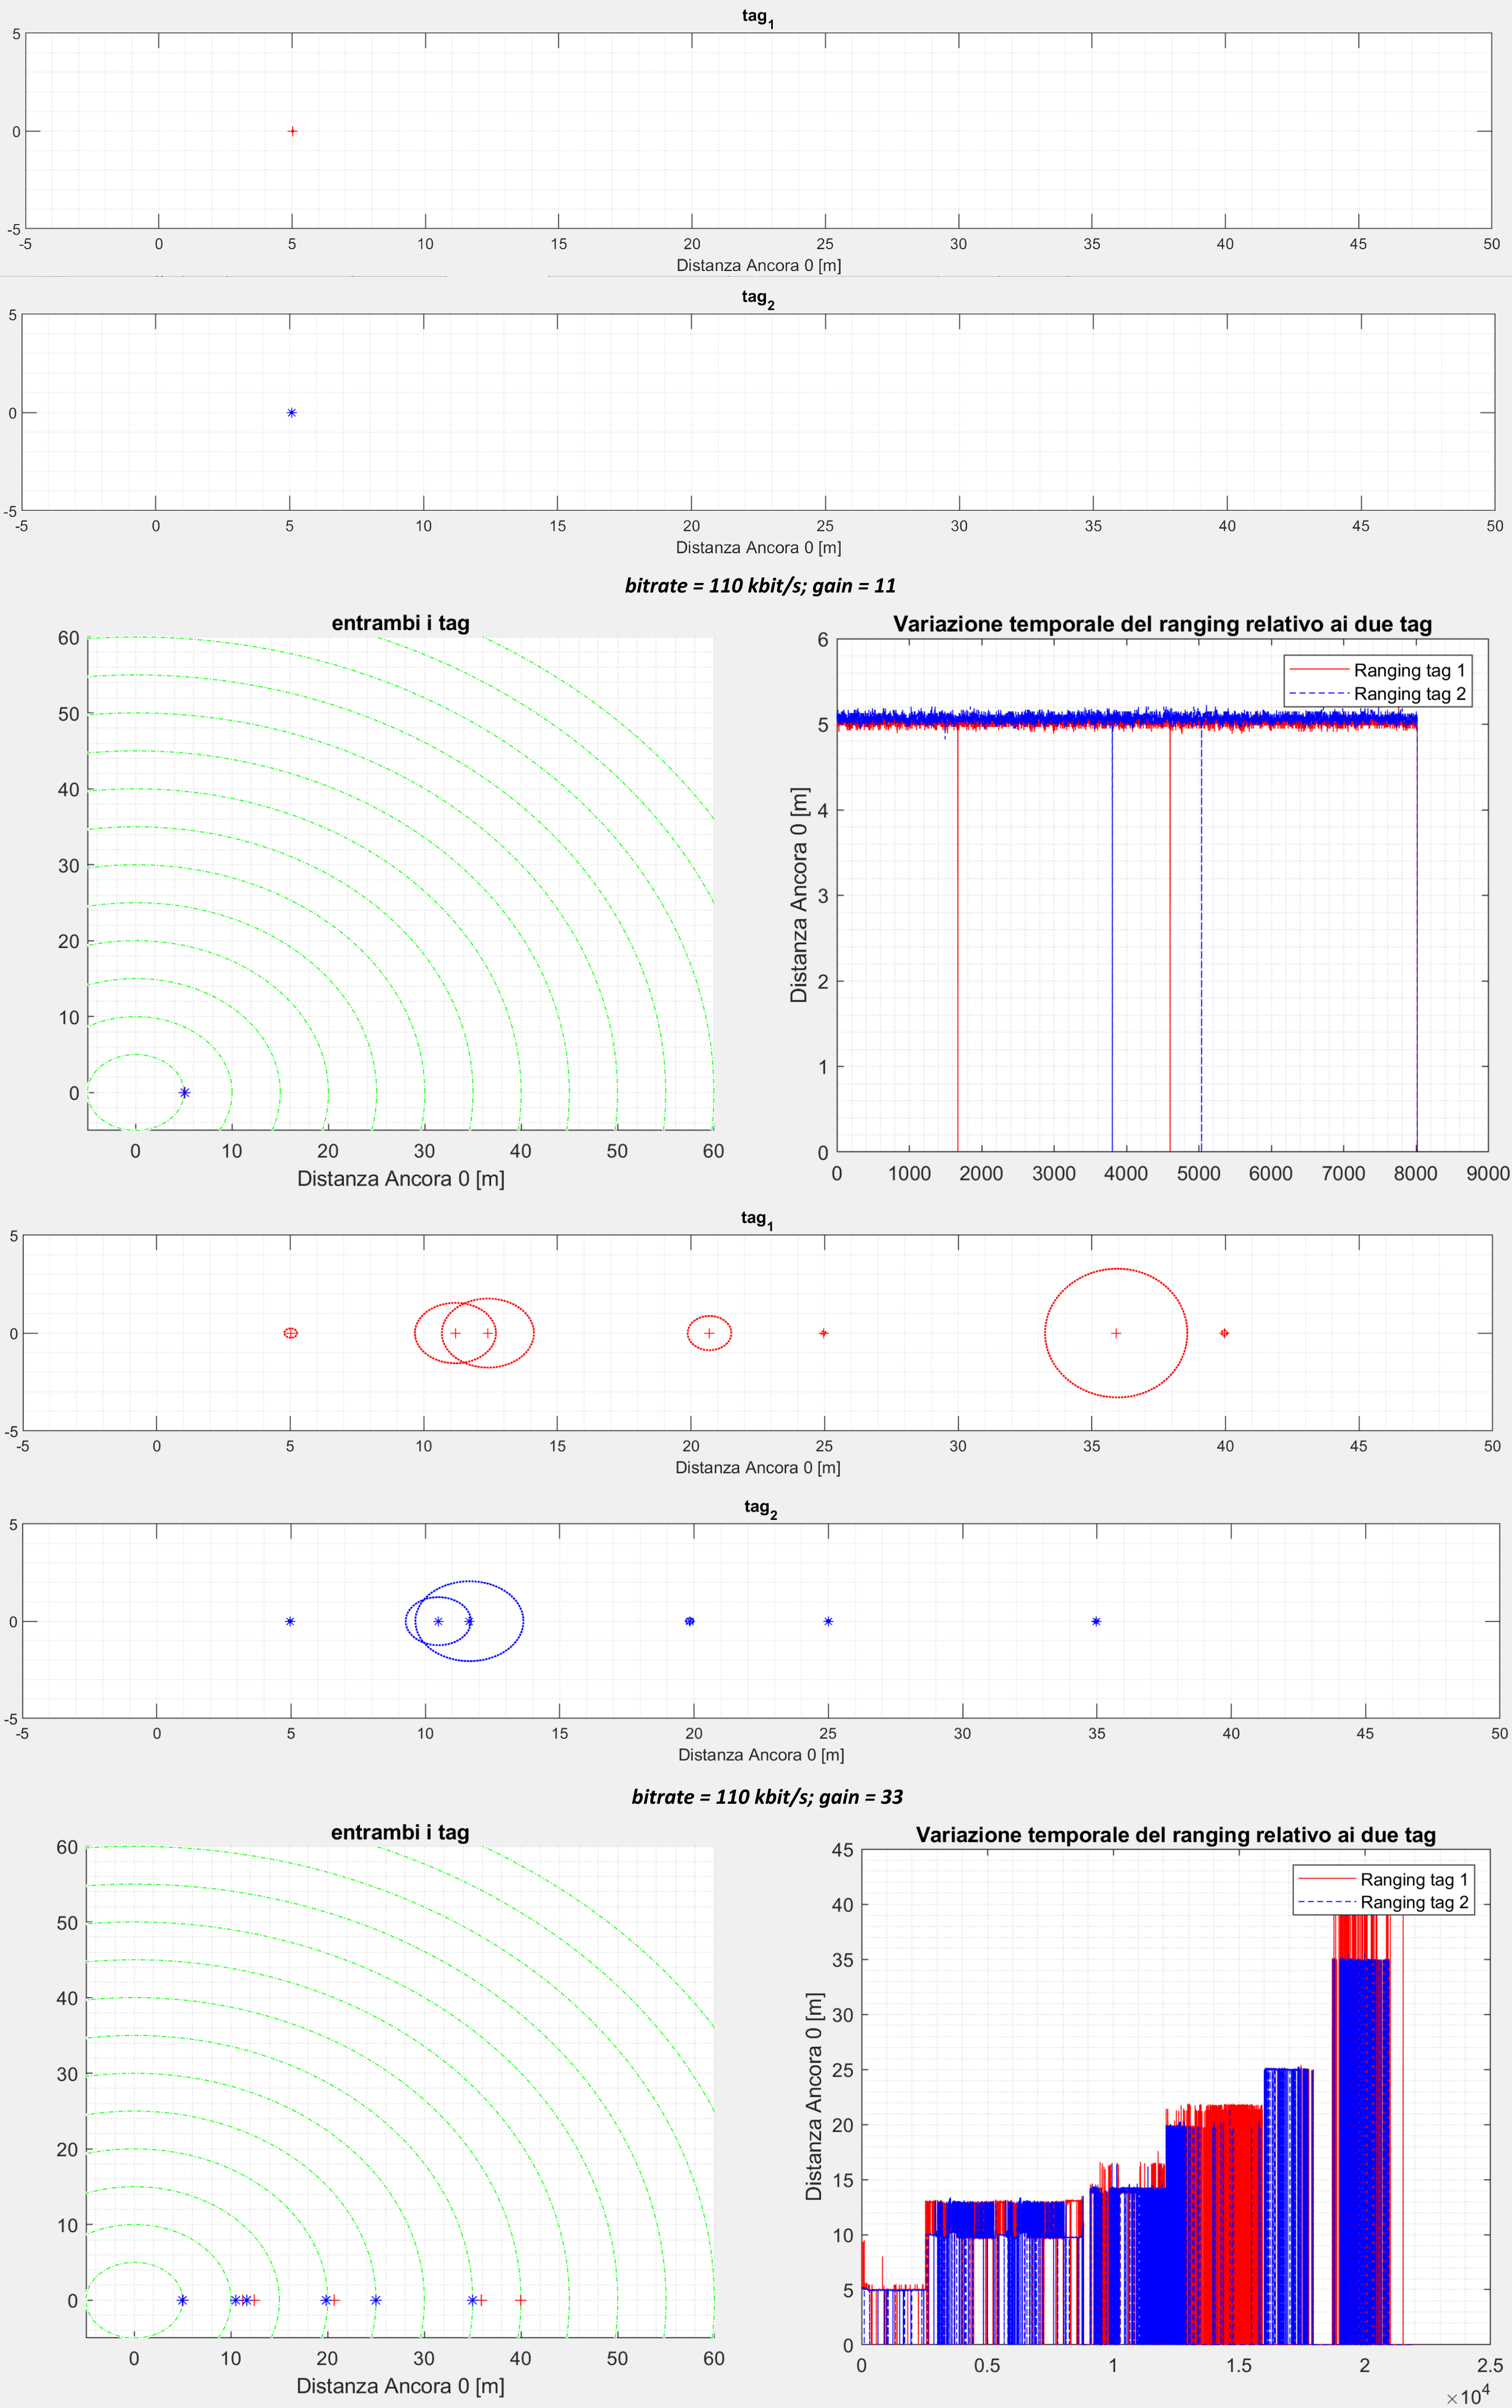
\includegraphics[scale=0.17]{EspOut110}
	 			\caption{\textbf{Figura 17:} esperimento di ranging outdoor [bitrate = 110 kbit/s; gain = 11.5 (sopra); gain = 33 (sotto)]. Per ogni  esperimento l'ultima immagine è posta per un confronto grafico tra la distanza calcolata dal ranging rispetto all'Ancora 0 e la distanza calcolata come $\sqrt{(x^2+y^2)}$, 						derivanti dal positioning\label{EspOut110}}
			\end{figure}
			
			\begin{figure}[H]
				\centering
				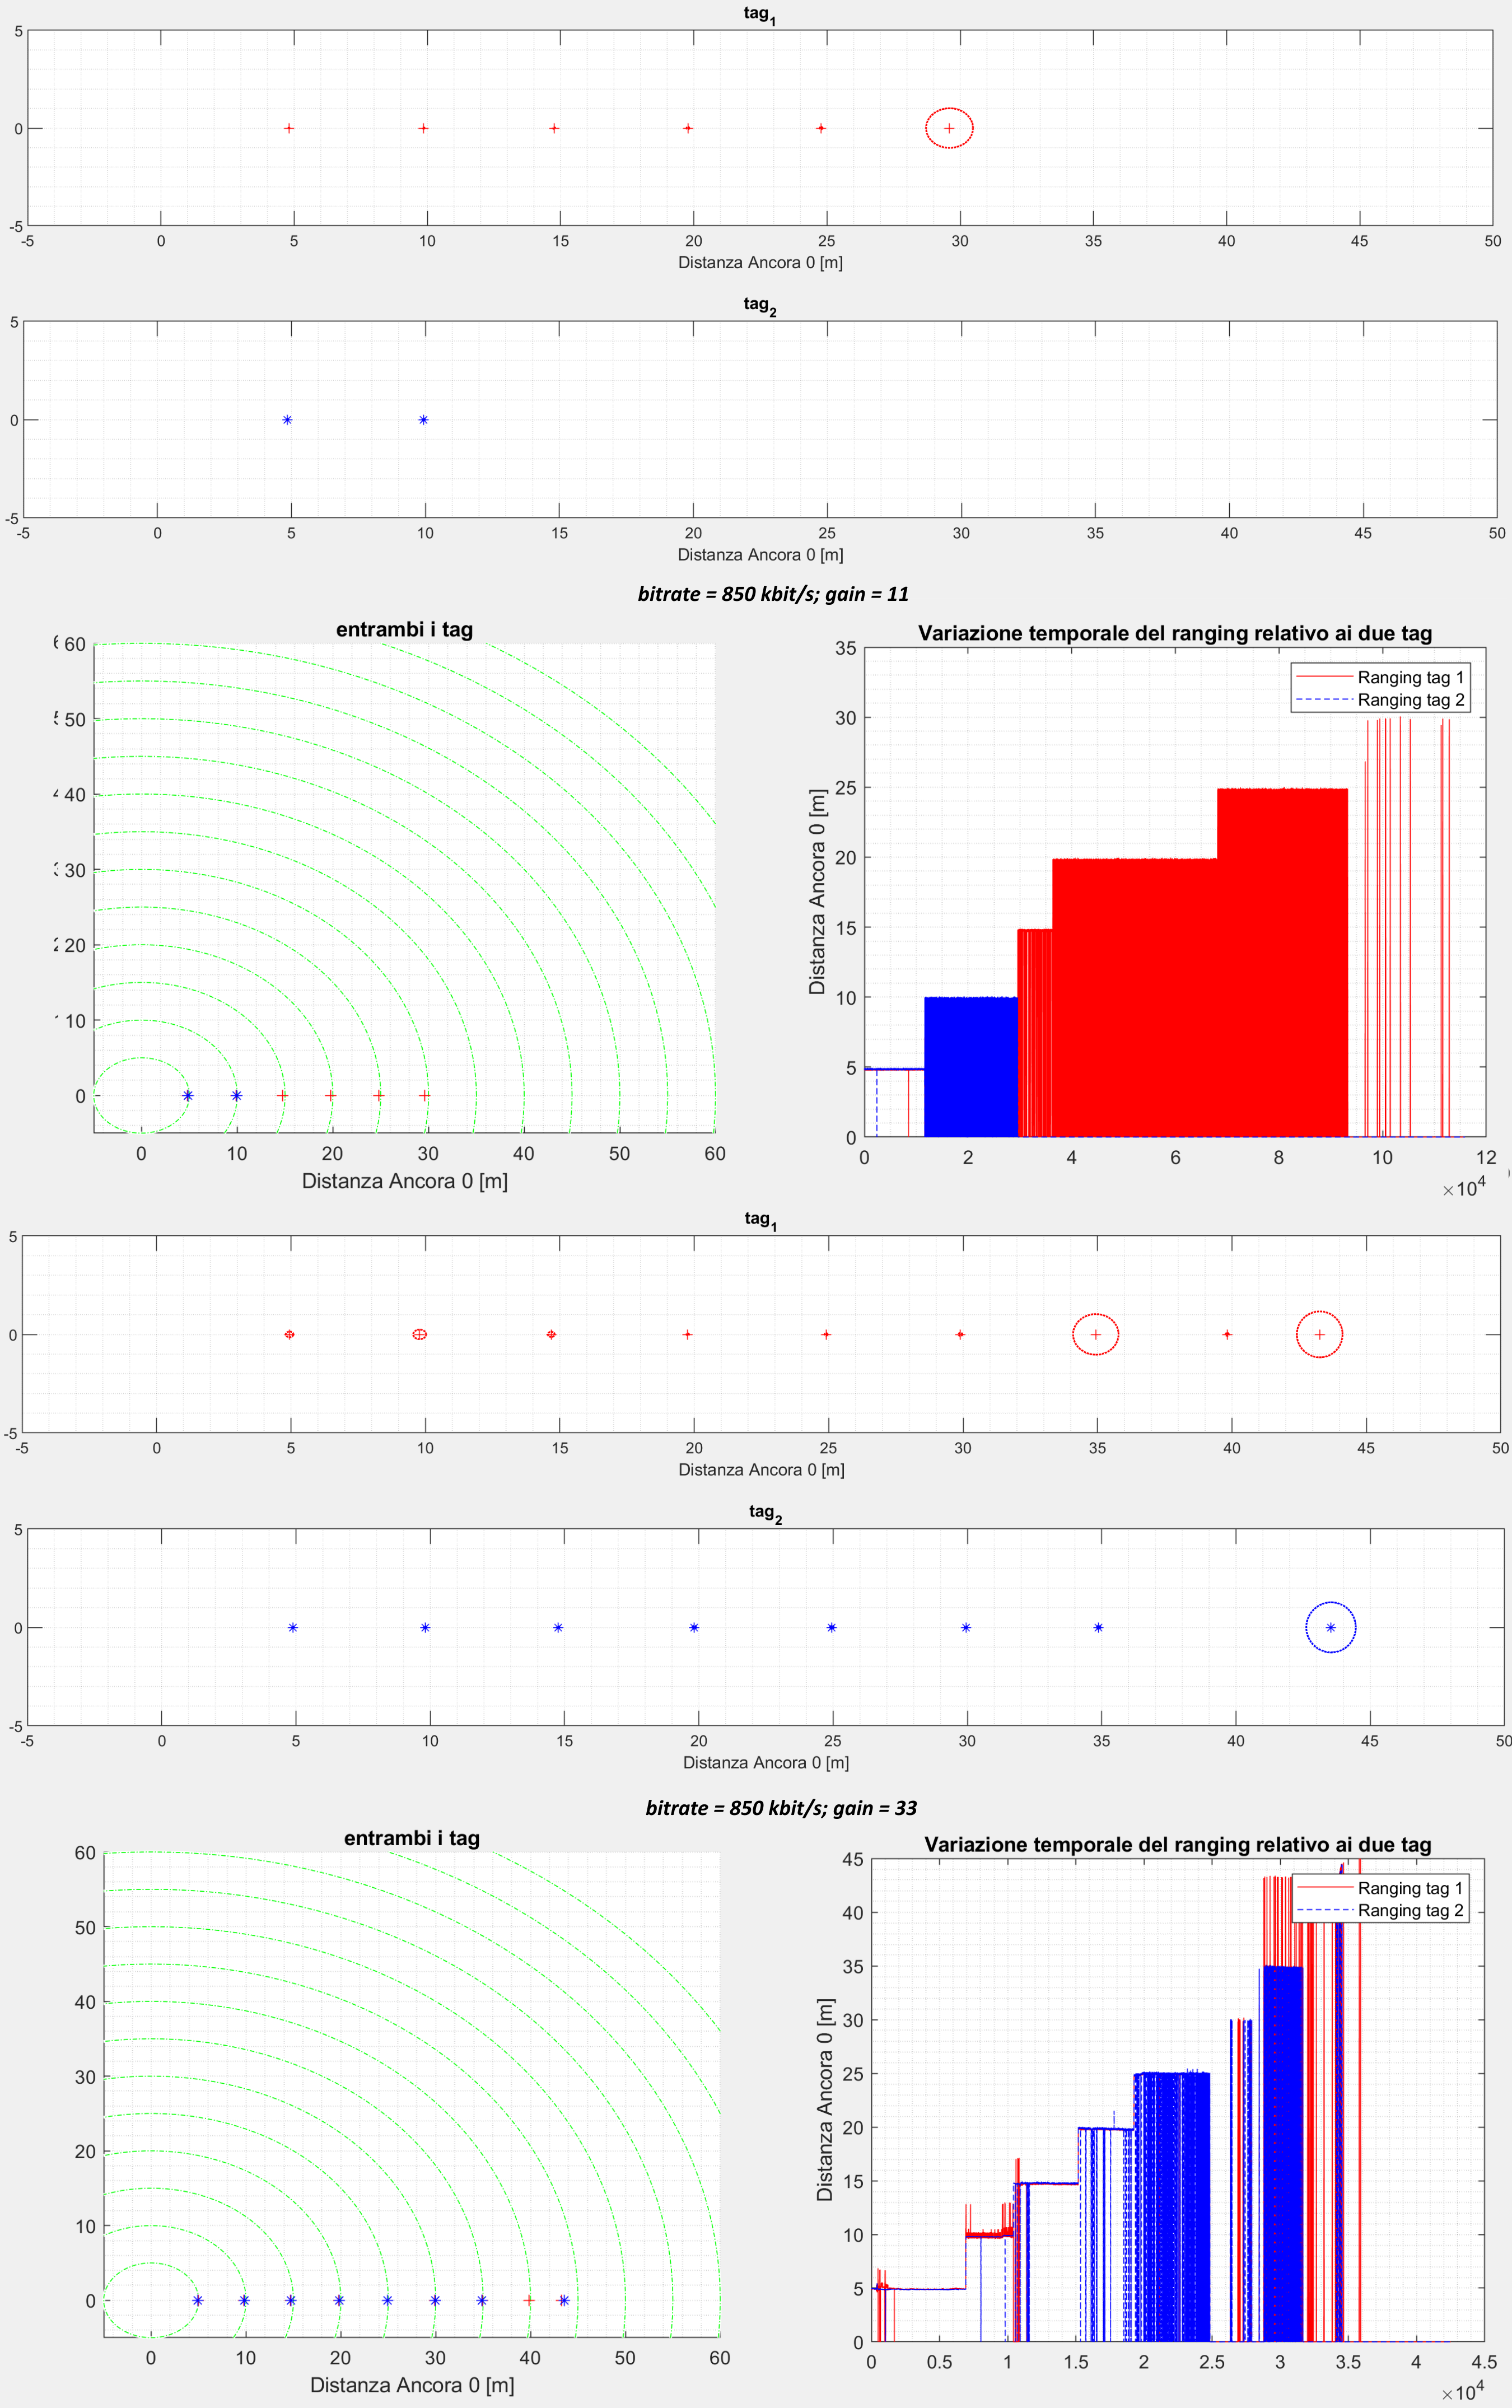
\includegraphics[scale=0.17]{EspOut850}
	 			\caption{\textbf{Figura 18:} esperimento di ranging outdoor [bitrate = 850 kbit/s; gain = 11.5 (sopra); gain = 33 (sotto)]. Per ogni  esperimento l'ultima immagine è posta per un confronto grafico tra la distanza calcolata dal ranging rispetto all'Ancora 0 e la distanza calcolata come $\sqrt{(x^2+y^2)}$, 						derivanti dal positioning\label{EspOut850}}
			\end{figure}

			\begin{figure}[H]
				\centering
				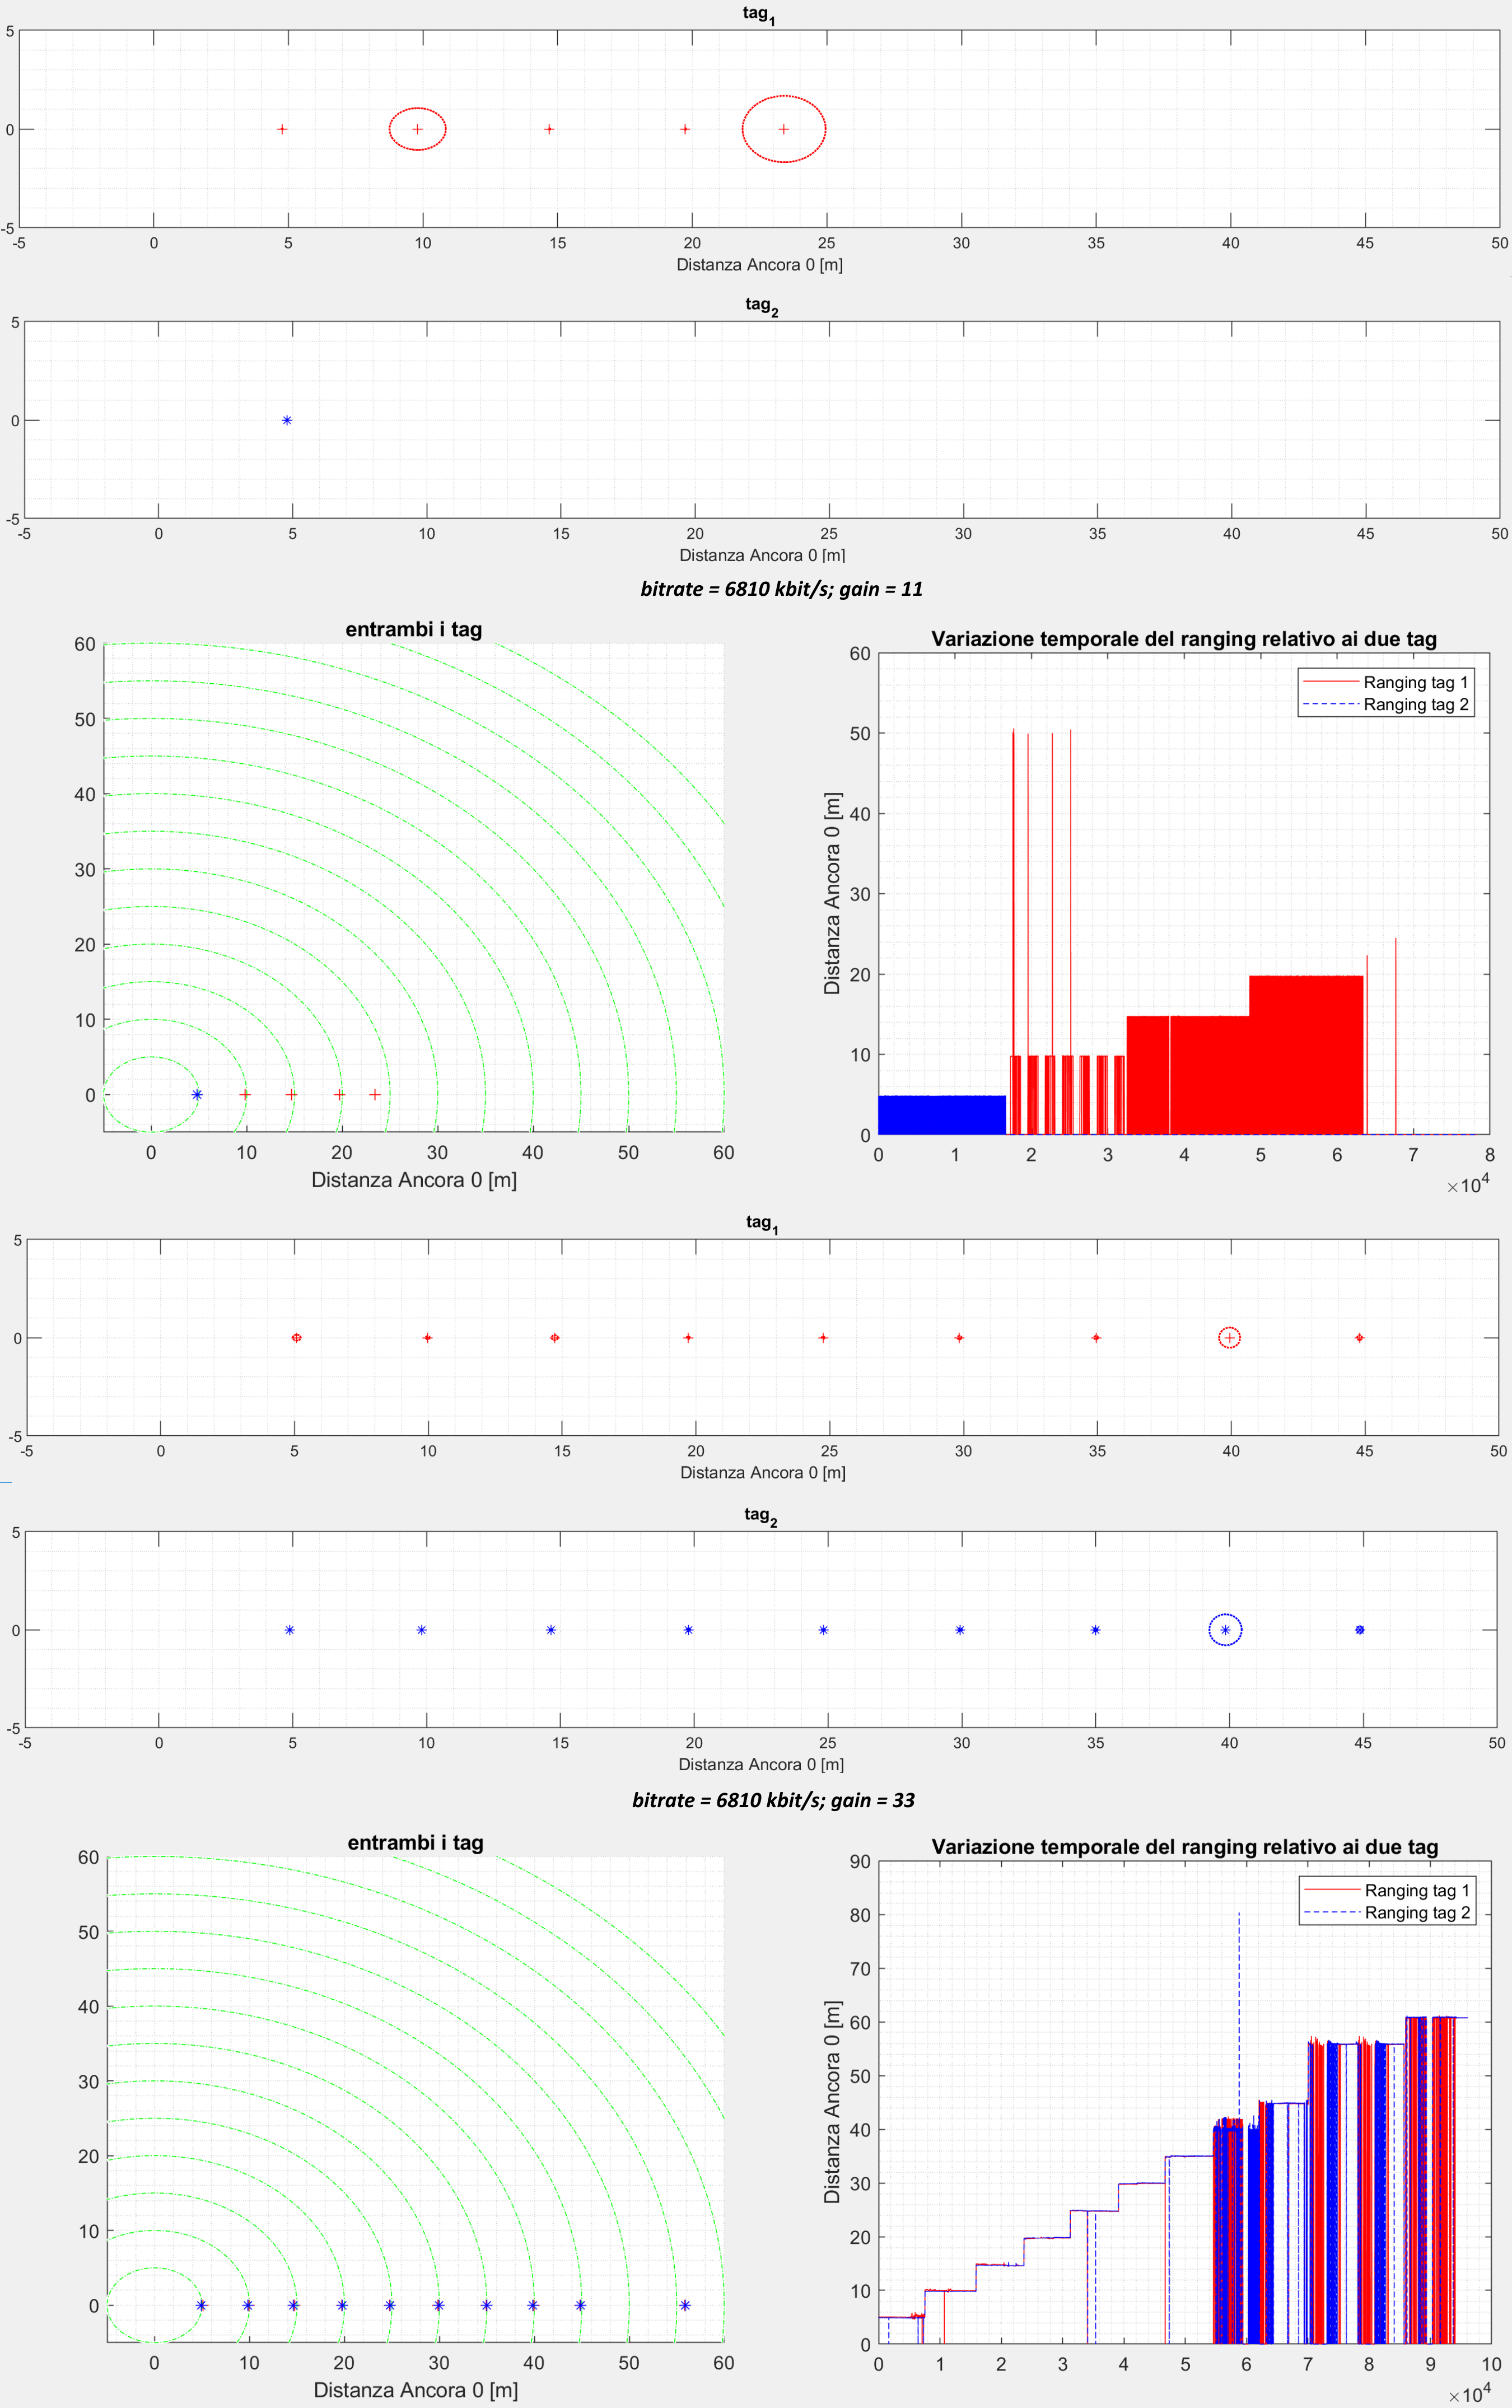
\includegraphics[scale=0.17]{EspOut6810}
	 			\caption{\textbf{Figura 19:} esperimento di ranging outdoor [bitrate = 6810 kbit/s; gain = 11.5 (sopra); gain = 33 (sotto)]. Per ogni  esperimento l'ultima immagine è posta per un confronto grafico tra la distanza calcolata dal ranging rispetto all'Ancora 0 e la distanza calcolata come $\sqrt{(x^2+y^2)}$, 						derivanti dal positioning \label{EspOut6810}}
			\end{figure}	
			Dall'andamento si nota, però, un'altra cosa interessante. In tutti i casi, infatti, al crescere del bitrate la distanza risulta aumentare per entrambi i casi di gain analizzati. Per semplicità viene riportata la  \textbf{\tablename~\ref{EspOutGain}} per mettere in evidenza questa caratteristica.

			\begin{table}[H]
					\centering
					\begin{tabular}{|c|c|c|c|c|c|c|}
						\hline
						\multicolumn{7}{|c|}{}\\
						\multicolumn{7}{|c|}{\textbf{\Large Distanza massima Ranging}}\\
						\multicolumn{7}{|c|}{}\\
						\hline
						\multirow{2}{*}{Gain}&							\multicolumn{2}{|c|}{Bitrate = 110 kbit/s}&										\multicolumn{2}{|c|}{Bitrate = 850 kbit/s}&								\multicolumn{2}{|c|}{Bitrate = 6810 kbit/s}\\
						\cline{2-7}
						&																tag\textsubscript{1}&tag\textsubscript{2}&										tag\textsubscript{1}&tag\textsubscript{2}&								tag\textsubscript{1}&tag\textsubscript{2}\\
						\hline
						11.5&														5 m                 &				5 m            &											30 m               &			10 m                  &									25 m                  &			5 m\\
						\hline
						33&															40 m              &				35 m          &													45 m                  &			45 m                  &									55 m                  &			55 m\\
						\hline
					\end{tabular}
					\caption{\textbf{Tabella 11: } Esito test sul ranging in termini di distanza massima raggiunta al variare del bitrate e del gain.\label{EspOutGain}}
			\end{table}
		\end{subsection}

		\begin{subsection}{Esperimento Positioning}

			Il secondo esperimento condotto all'esterno ha avuto l'obiettivo di investigare il comportamento dell'algoritmo di positioning. Tale esperimento è stato eseguito in due fasi distinte.\\ In un primo momento sono state poste le prime tre ancore ai vertici di un quadrato di lato pari a 20 m. La quarta è stata posta più 			in alto, leggermente decentrata rispetto al baricentro del poligono. La \textbf{\figurename~\ref{EspOutConfig}} chiarisce la configurazione adottata. La linea verde in figura indica il percorso seguito: ci si è mossi circa lungo la diagonale del quadrato fermandoci ogni 5m, con i tag posti ad un'altezza di circa $2m				$ da terra. 
			Per ogni dispositivo è stata impostata la configurazione di parametri UWB ottimale ( \textbf{bitrate} = $6810$, \textbf{gain} = $33$, \textbf{channel} = 5, \textbf{prf} = 64, \textbf{plen} = 64). In tempo reale è stato possibile riscontrare graficamente l'andamento del test lungo tutto il percorso grazie 							all'utilizzo dello sketch su Processing 3 già descritto. \\ Il risultato è riassuto in \textbf{\figurename~\ref{EspOutPos1}}. Nella parte superiore viene mostrato il percorso ottenuto in fase di allontanamento dall'ancora 0, mentre in quella inferiore in fase di riavvicinamento. Le due differiscono per il punto in cui 								graficamente è stata posta l'origine, in quanto prima dell'esperimento non si era consapevoli del fatto che si sarebbero raggiunte tali distanze. Successivamente è stata riposizionata la grafica. 

			\begin{figure}[H]
				\centering
				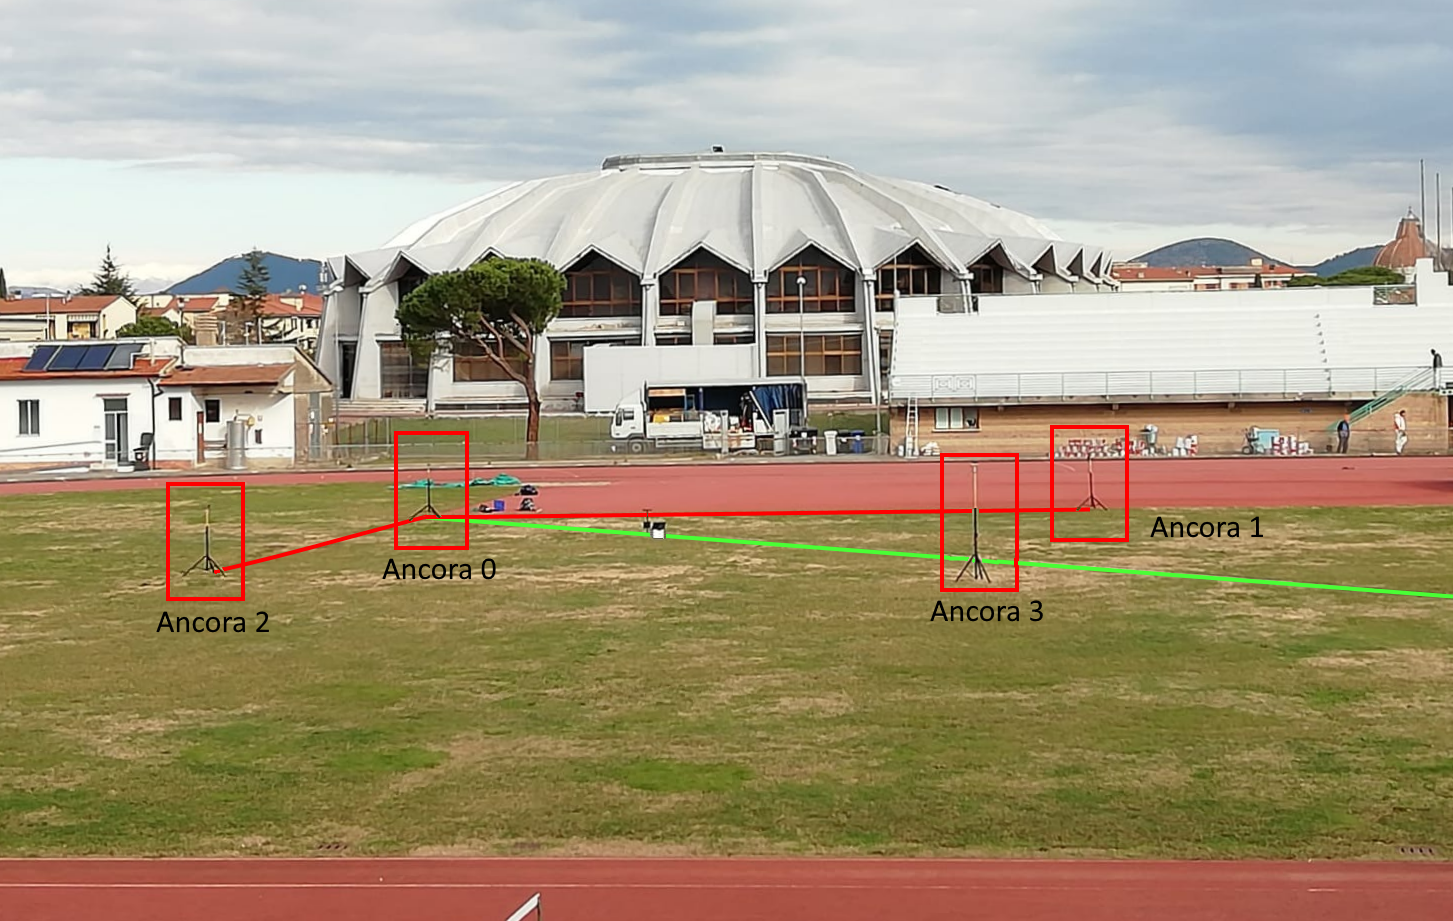
\includegraphics[scale=0.33]{EspOutConfig}
	 			\caption{\textbf{Figura 20:} esperimento outdoor per il testing del positioning\label{EspOutConfig}}
			\end{figure}
			Già dalla figura è possibile evincere discretamente la buona riuscita dell'esperimento. La distanza coperta risulta essere notevole, ma ancor di più è evidente una buona trilaterazione dei due tag. Infatti, posti a una distanza di $40 cm$ l'uno dall'altro, vengono plottati in figura come ben distinti. Ciò è 									particolarmente visibile nella parte inferiore dell'immagine. Da quest'ultima però si nota anche come l'algoritmo di positioning abbia bisogno di maggior tempo per andare a regime quando il punto di partenza del tag si trova lontano rispetto alle ancore. Nella parte finale del percorso, infatti, le misure ottenute 					sono poco accurate e l'algoritmo sembra aver un transitorio più lungo.

			\begin{figure}[H]
				\centering
				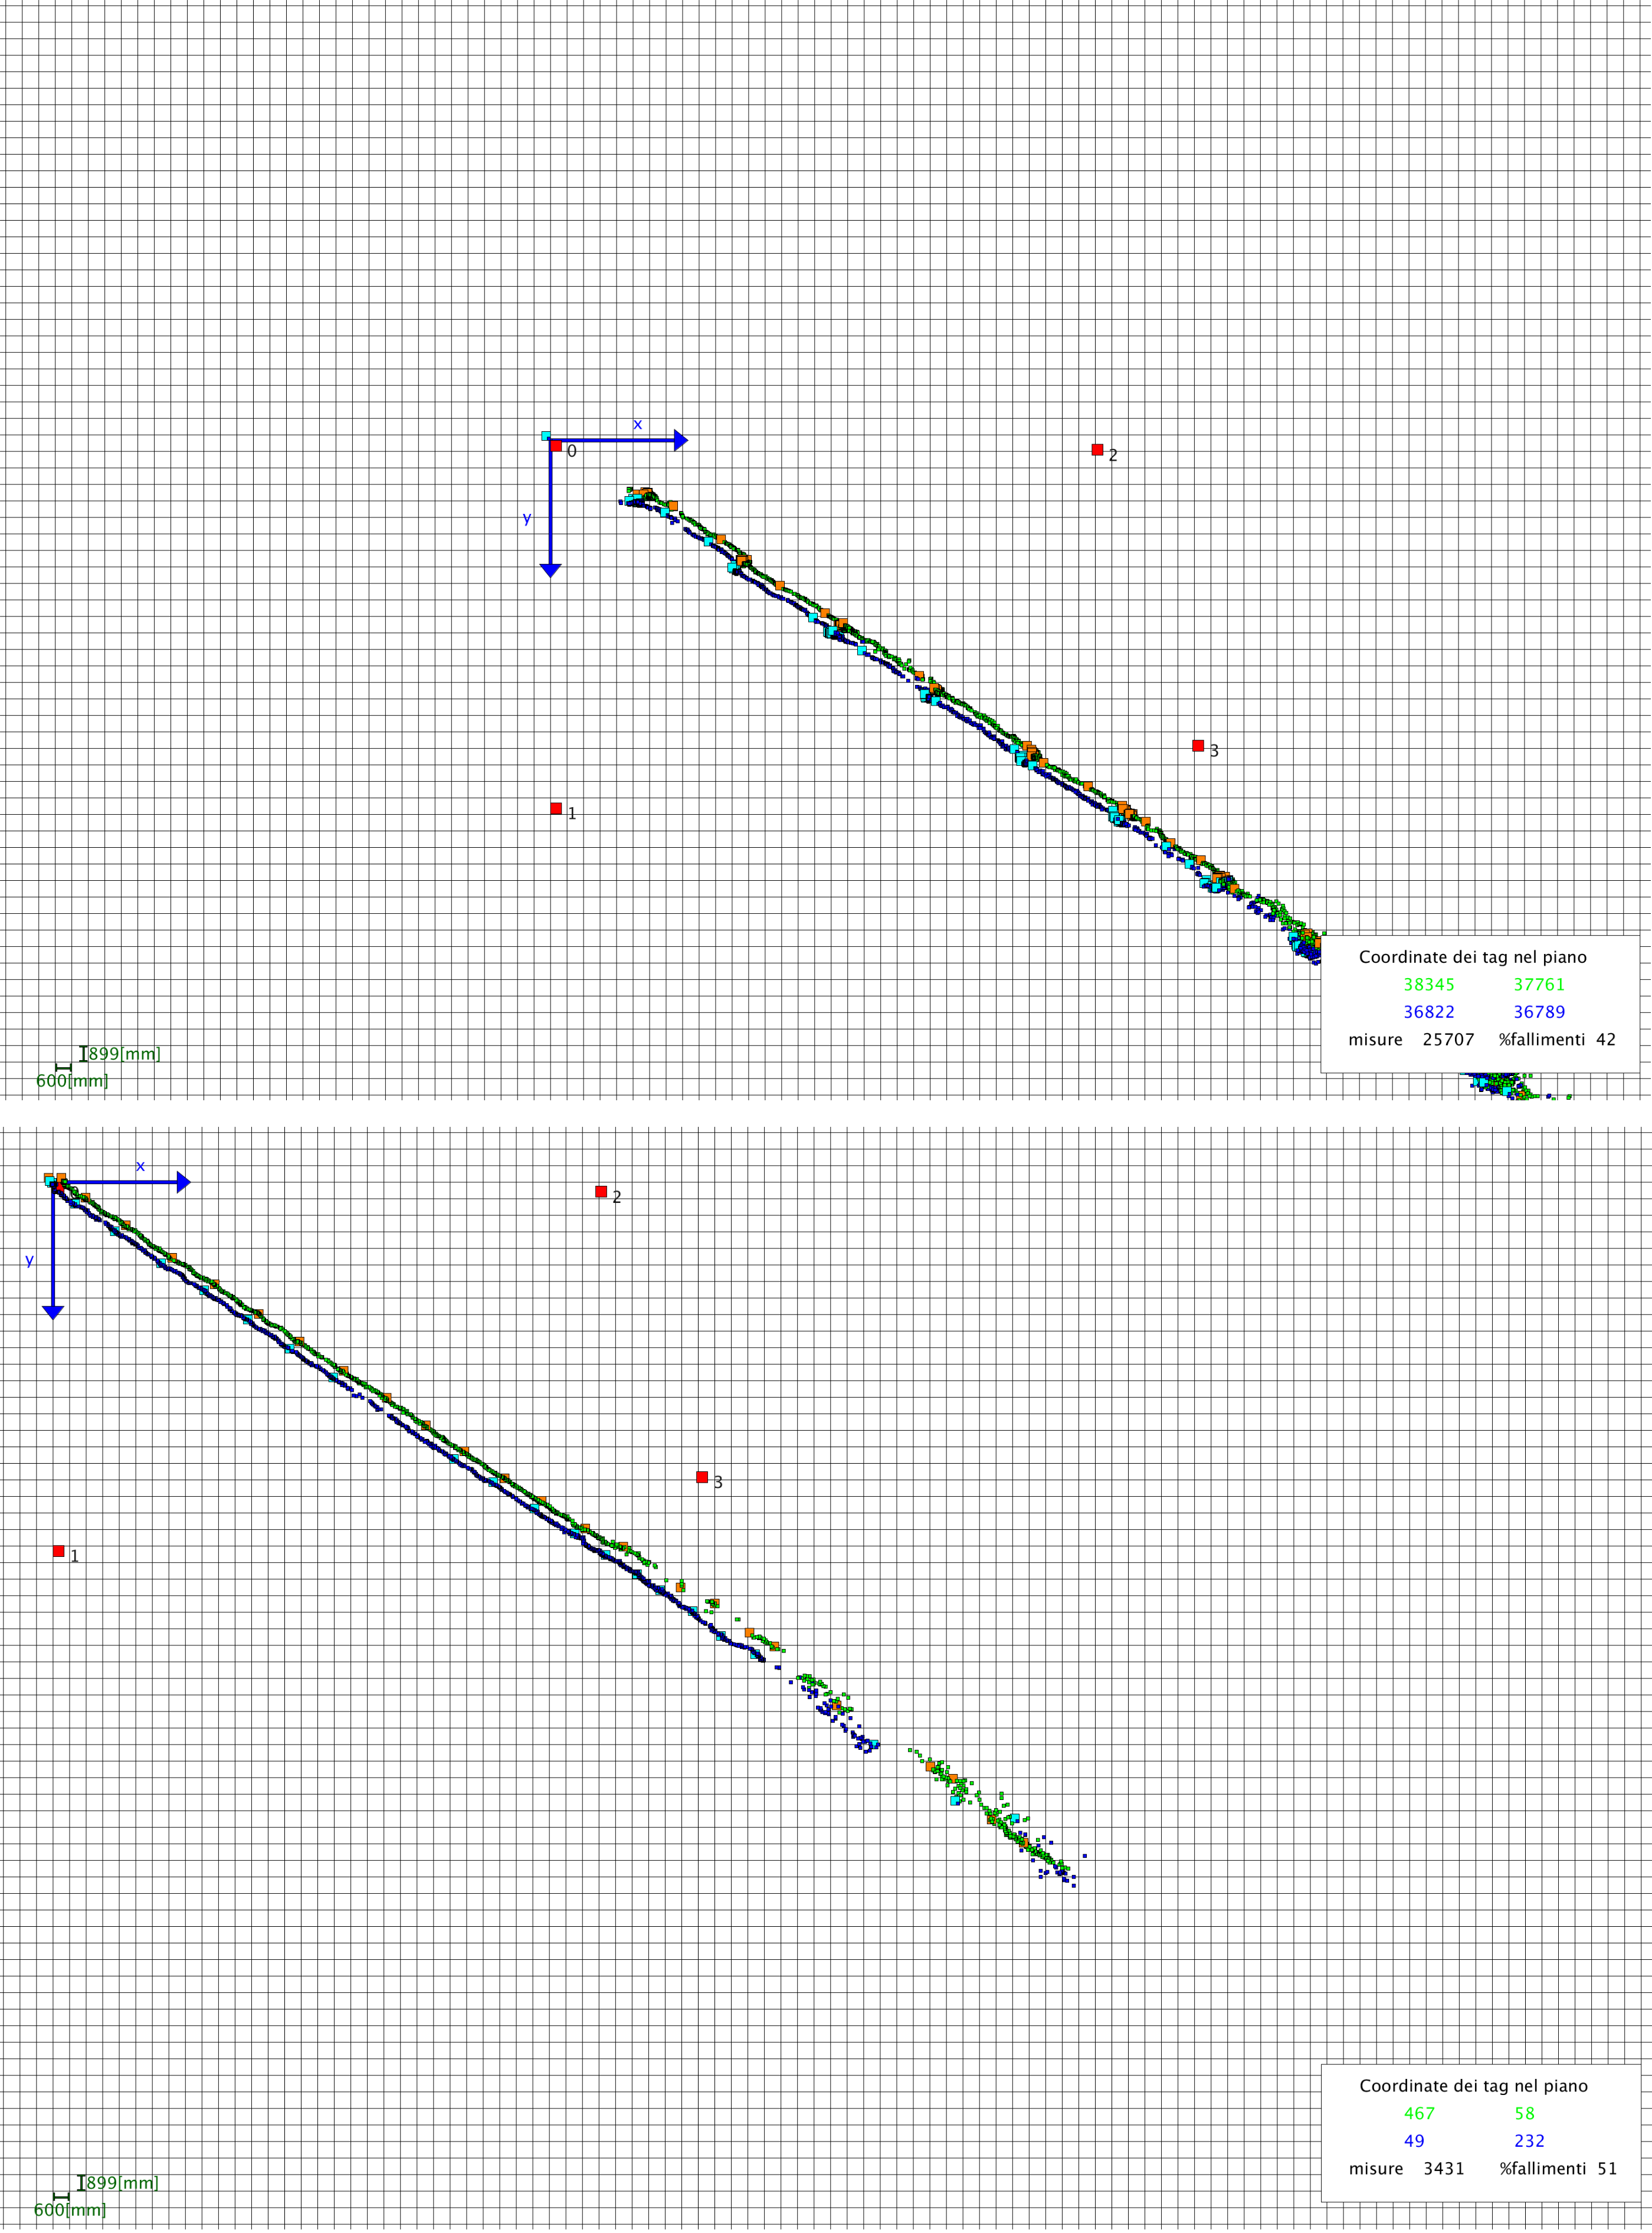
\includegraphics[scale=0.2]{EspOutPos1}
	 			\caption{\textbf{Figura 21:} esperimento positioning con distanza Ancora 0 - Ancora 1 = Ancora 0 - Ancora 2 = 20 m. Fase di allontanamento dall'Ancora 0 nella parte superiore dell'imagine, di avvicinamento nella parte inferiore\label{EspOutPos1}}
			\end{figure}

			Nella \textbf{\figurename~\ref{EspOutPos20}} sono graficate le posizioni che i tag assumono nel piano x, y. La parte superiore mostra dei cerchi centrati nella media delle posizioni, con raggi pari alla deviazione standard. Si nota che le misure assumono deviazioni standard differenti lungo il tragitto. In 							particolare, la dispersione aumenta nei dati ricavati in corrispondenza dei valori delle ascisse pari a $15$, $20$ e $25$ $m$ e poi ritorna a diminuire. Questo potrebbe essere dovuto al fatto che i tag si trovavano pressocchè al di sotto dell’antenna 4. Infatti, in questa circostanza, il suo angolo di radiazione 							risulta elevato. Ciò influisce negativamente nella comunicazione. Da  distanze superiori a $40m$ rispetto all'ancora 0, i valori sembrano essere più precisi ma l’algoritmo di positioning mostra una percentuale di fallimenti molto elevata. Queste conclusioni sono valide per entrambi i tag. \\ In tutti gli esperimenti 					condotti, la coordinata z è sempre risultata quella stimata in maniera peggiore. Inoltre, dalla \textbf{\tablename~\ref{EspOut20}} si denota come da 50 m in poi, essa presenti un valore inverosimile ed una deviazione standard superiore a 5 metri. 
			\begin{table}[H]
				\centering
\resizebox*{1.0\textwidth}{!}{
				\begin{tabular}{|c||c|c|c||c|c|c|c||}
					\hline
					\multicolumn{8}{|c|}{}\\
					\multicolumn{8}{|c|}{\textbf{\Large Tag 1}}\\
					\multicolumn{8}{|c|}{}\\
					\hline
					&\multicolumn{3}{|c||}{Coordinate [m]}&											\multicolumn{4}{|c||}{Distanze [m]}\\
					\hline
					Distanza&x& 				y& 				z& 														d0& 				d1&				d2&			d3\\
					ancora 0 [m]&&&&&&&\\
					\hline
					5&3.643$\pm$0.114&3.165$\pm$0.066&-0.157$\pm$0.358&			4.761$\pm$0.100&16.932$\pm$1.574&16.226$\pm$0.197&24.400$\pm$0.127\\
					\hline
					10&7.126$\pm$0.032&6.783$\pm$0.031&-0.077$\pm$0.353&			9.862$\pm$0.037&14.701$\pm$0.030&14.114$\pm$0.037&19.442$\pm$0.0384\\
					\hline
					15&10.689$\pm$0.039&6.783$\pm$0.031&0.104$\pm$0.406&			14.916$\pm$0.083&14.184$\pm$1.832&13.498$\pm$0.031&14.570$\pm$0.040\\
					\hline
					20&14.740$\pm$1.209&14.379$\pm$1.129&0.539$\pm$0.282&			20.653$\pm$1.690&15.644$\pm$2.670&14.972$\pm$0.808&9.344$\pm$1.322\\
					\hline
					25&19.079$\pm$1.634&18.637$\pm$1.476&1.098$\pm$1.475&			26.750$\pm$2.113&19.074$\pm$2.872&18.615$\pm$1.575&5.490$\pm$0.678\\
					\hline
					30&22.087$\pm$1.350&21.492$\pm$1.385&1.603$\pm$0.522&			30.719$\pm$1.328&22.543$\pm$4.638&21.743$\pm$1.611&5.426$\pm$1.059\\
					\hline
					35&24.626$\pm$0.1550&24.200$\pm$0.096&1.729$\pm$0.734&		35.026$\pm$0.051&24.908$\pm$0.029&24.772$\pm$0.044&7.555$\pm$0.031\\
					\hline
					40&27.898$\pm$0.242&27.500$\pm$0.225&2.030$\pm$2.098&			39.846$\pm$0.158&29.067$\pm$1.565&28.929$\pm$0.104&11.626$\pm$0.129\\
					\hline
					45&31.076$\pm$0.341&30.948$\pm$0.470&4.062$\pm$3.831&			44.933$\pm$0.066&33.490$\pm$0.075&33.525$\pm$0.057&16.496$\pm$0.052\\
					\hline
					50&34.382$\pm$0.673&34.717$\pm$0.824&1.722$\pm$5.818&			49.814$\pm$1.050&37.973$\pm$0.937&38.148$\pm$1.016&21.315$\pm$1.024\\
					\hline
					55&37.480$\pm$0.558&38.213$\pm$0.649&-3.030$\pm$5.843&		54.614$\pm$0.053&42.353$\pm$0.028&42.624$\pm$0.070&25.973$\pm$0.048\\
					\hline
					60&39.186$\pm$0.9612&39.175$\pm$1.315&15.694$\pm$3.554&		59.182$\pm$0.053&46.797$\pm$0.044&47.017$\pm$0.056&30.517$\pm$0.050\\
					\hline
					\multicolumn{8}{|c|}{}\\
					\multicolumn{8}{|c|}{\textbf{\Large Tag 2}}\\
					\multicolumn{8}{|c|}{}\\
					\hline
					&\multicolumn{3}{|c||}{Coordinate [m]}&											\multicolumn{4}{|c||}{Distanze [m]}\\
					\hline
					Distanza&x& 				y& 				z& 														d0& 				d1&				d2&			d3\\
					ancora 0 [m]&&&&&&&\\
					\hline
					5&3.291$\pm$0.089&3.539$\pm$0.068&-0.107$\pm$0.329&			4.790$\pm$0.097&16.495$\pm$1.287&16.684$\pm$0.167&24.478$\pm$0.096\\
					\hline
   					 10&6.854$\pm$ 0.037&7.244$\pm$ 0.028&-0.124$\pm$0.391&			9.986$\pm$0.021&14.153$\pm$0.031&14.551$\pm$0.038&19.479$\pm$0.034\\
  					\hline 
					15&10.347$\pm$0.035&10.738$\pm$0.039&0.128$\pm$0.352&			14.942$\pm$0.050&13.583$\pm$0.896&13.981$\pm$0.034&14.721$\pm$0.045\\
					\hline
   					20&14.455$\pm$1.269&14.766$\pm$1.181&0.528$\pm$0.305&			20.668$\pm$1.828&15.037$\pm$0.851&15.381$\pm$0.785&9.672$\pm$1.273\\
					\hline
   					25&18.723$\pm$1.649&18.981$\pm$ 1.522&1.064$\pm$0.452&			26.641$\pm$2.116&18.533$\pm$1.647&18.953$\pm$1.573&5.985$\pm$0.649\\
					\hline
   					30&21.317$\pm$1.185&21.399$\pm$1.088&1.534$\pm$0.541&			30.614$\pm$1.278&21.794$\pm$2.064&22.036$\pm$1.516&5.840$\pm$0.920\\
					\hline
   					35&4.458$\pm$0.251&24.402$\pm$0.161&2.084$\pm$1.163&			34.965$\pm$0.032&24.857$\pm$0.303&25.027$\pm$0.028&7.823$\pm$0.034\\
					\hline
   					40&27.600$\pm$0.289&27.860$\pm$0.198&2.080$\pm$2.431&			39.883$\pm$0.153&28.861$\pm$0.911&29.262$\pm$0.130&11.885$\pm$0.124\\
					\hline
   					45&30.794$\pm$0.422&31.450$\pm$0.418&2.412$\pm$3.833&			44.886$\pm$0.035&33.195$\pm$0.087&33.666$\pm$0.062&16.615$\pm$0.046\\
					\hline
   					50&34.100$\pm$0.669&34.826$\pm$0.694&1.914$\pm$6.036&			49.673$\pm$1.053&37.673$\pm$0.947&38.118$\pm$ 1.032&21.292$\pm$1.012\\
					\hline
   					55&36.836$\pm$0.738&38.061$\pm$1.060&4.827$\pm$8.008&			54.583$\pm$0.052&42.117$\pm$0.091&42.768$\pm$0.072&26.079$\pm$0.046\\
					\hline
   					60&39.054$\pm$0.913&39.746$\pm$1.353&14.771$\pm$4.575&		59.249$\pm$0.070&46.688$\pm$0.045&47.244$\pm$0.048&30.641$\pm$0.054\\
					\hline
				\end{tabular}
}
				\caption{\textbf{Tabella 12:} Dati relativi all'esperimento positioning con distanza Ancora 0 - Ancora 1 = Ancora 0 - Ancora 2 = 20 m\label{EspOut20}}
			\end{table}

\begin{table}[H]
				\centering
				\begin{tabular}{|c||c|c||c|c|}
					\hline
					\multicolumn{5}{|c|}{}\\
					\multicolumn{5}{|c|}{\textbf{\Large Distanze dall'Ancora 0}}\\
					\multicolumn{5}{|c|}{}\\
					\hline
					\multirow{2}{*}{Reale}&\multicolumn{2}{|c||}{Tag 1}&	\multicolumn{2}{|c|}{Tag2}\\
					\cline{2-5}
					&$\sqrt{(x^2+y^2)}$& d0& 		$\sqrt{(x^2+y^2)}$& d0\\
					\hline
					5&4.826&    				4.761&      4.833&    				  4.7907\\
					\hline
   					10&9.838&   				9.862&      9.973 &   				  9.9868\\
					\hline
   					15&14.892&  				14.916&    14.913&   			 14.9422\\
					\hline
   					20&620.592& 				20.653&    20.664&  				 20.6687\\
					\hline
   					25&26.671&   				26.751&    26.662&   			 26.6418\\
					\hline
   					30&30.818&   				30.719&    30.206&   			 30.6150\\
					\hline
   					35&34.527&   				35.026&    34.550&   			 34.9654\\
					\hline
   					40&39.173&   				39.846&    39.217&   			 39.8833\\
					\hline
   					45&43.857&   				44.933&    44.016&   			 44.8861\\
					\hline
   					50&48.862&   				49.814&    48.742&   			 49.6737\\
					\hline  					
					55&53.525&   				54.614&    52.968&  				 54.5836\\
					\hline
   					60&55.409&   				59.182&    55.723&   			 59.2491\\
					\hline
				\end{tabular}
				\caption{\textbf{Tabella 13:} Confronto tra ranging e distanza planare rispetto all'Ancora 0; riferiti all'esperimento positioning con distanza Ancora 0 - Ancora 1 = Ancora 0 - Ancora 2 = 20 m. \label{EspOut20}}
			\end{table}

			Si è cercato di caratterizzare l’esito dell’algoritmo di positioning in funzione della distanza tra le ancore. Perciò, in un secondo momento, sono state installate le prime tre ancore ai vertici di un quadrato di lato pari a $30m$, lasciando invariata la posizione della quarta ancora. È stato effettuato lo stesso 								esperimento descritto in precedenza. Dalla \textbf{\figurename~\ref{EspOutPos30}} si nota un incremento della dispersione dei valori man mano che aumenta la distanza dall’origine. In particolare, in corrispondenza di $55m$, la deviazione massima supera i 2 metri e si osserva un notevole aumento dei 							fallimenti.  Anche in questo caso è stato utilizzato lo strumento dato da Processing 3 per valutare in tempo reale l'esperimento. In \textbf{\figurename~\ref{EspOutPos2}}, si può notare come per lunghi tratti anche in questo caso i due tag sono facilmente discindibili. Ma giunti a distanze superiori a 50 m 							dall'ancora 0, nonostante un ranging plausibile, le posizioni risultano corrotte. L'algoritmo di trialaterazione, mappava i dati in una posizione differente da quella in cui i tag realmente si trovavano. Questo è visibile dall'estesa nuvola di punti segnalata in figura.

			\begin{figure}[H]
				\centering
				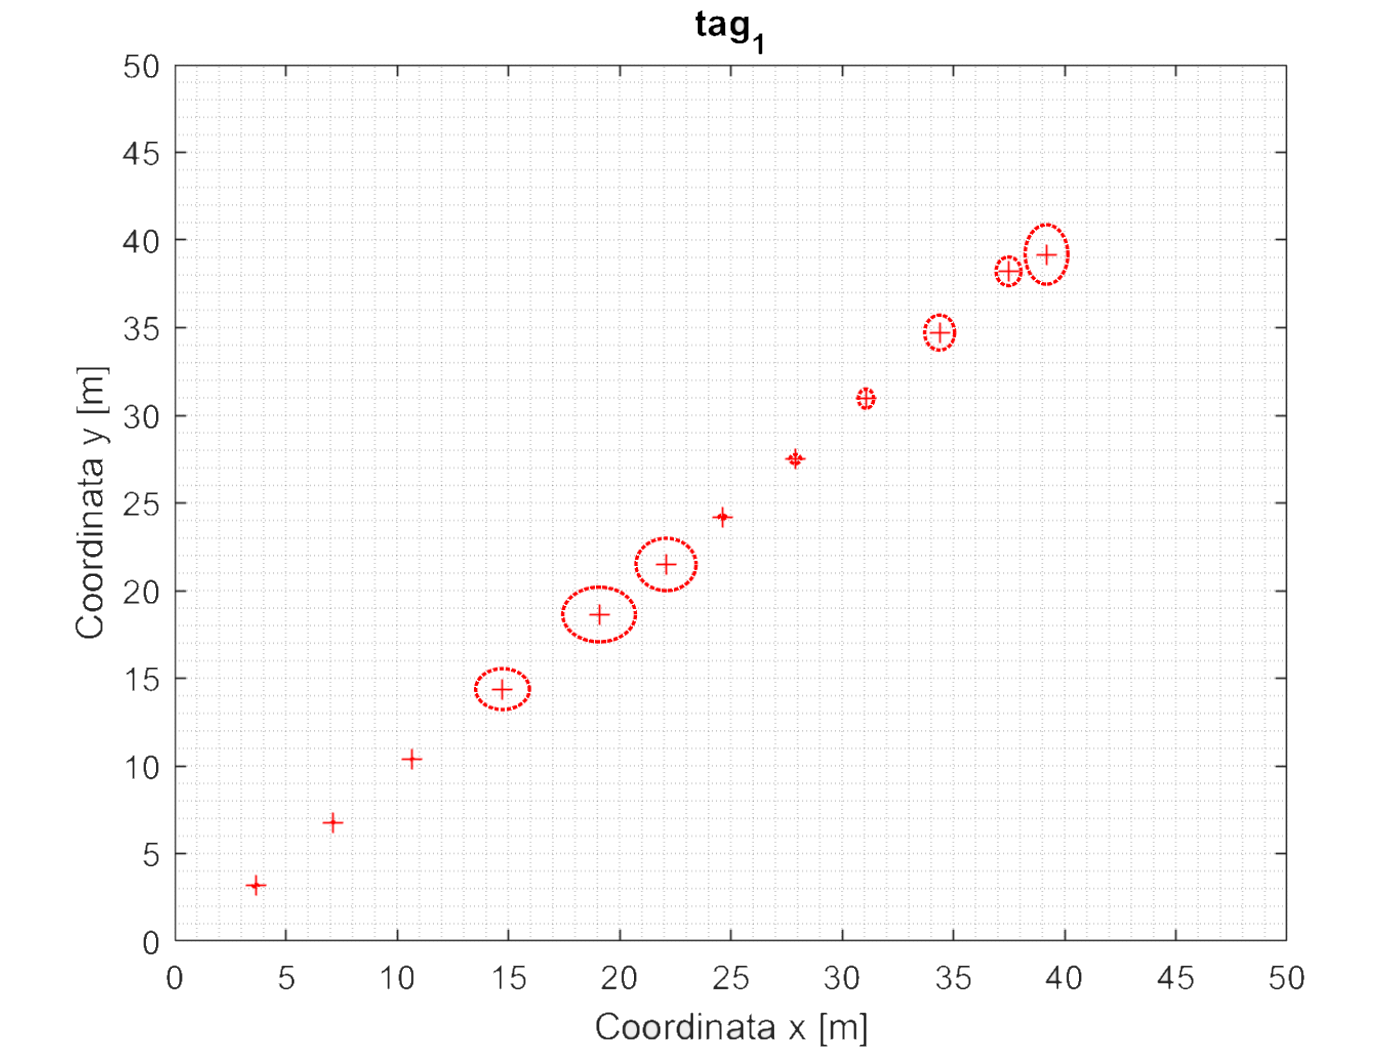
\includegraphics[scale=0.3]{EspOutPos20_1}
	 			\caption{\textbf{Figura 22:} posizione del tag 1 nel piano \textit{xy} durante l'esperimento sul positioning con distanza Ancora 0 - Ancora 1 = Ancora 0 - Ancora 2 = 20 m. Gli ellissi hanno semiassi corrispondenti alle deviazioni.\label{EspOutPos20_1}}
			\end{figure}

			\begin{figure}[H]
				\centering
				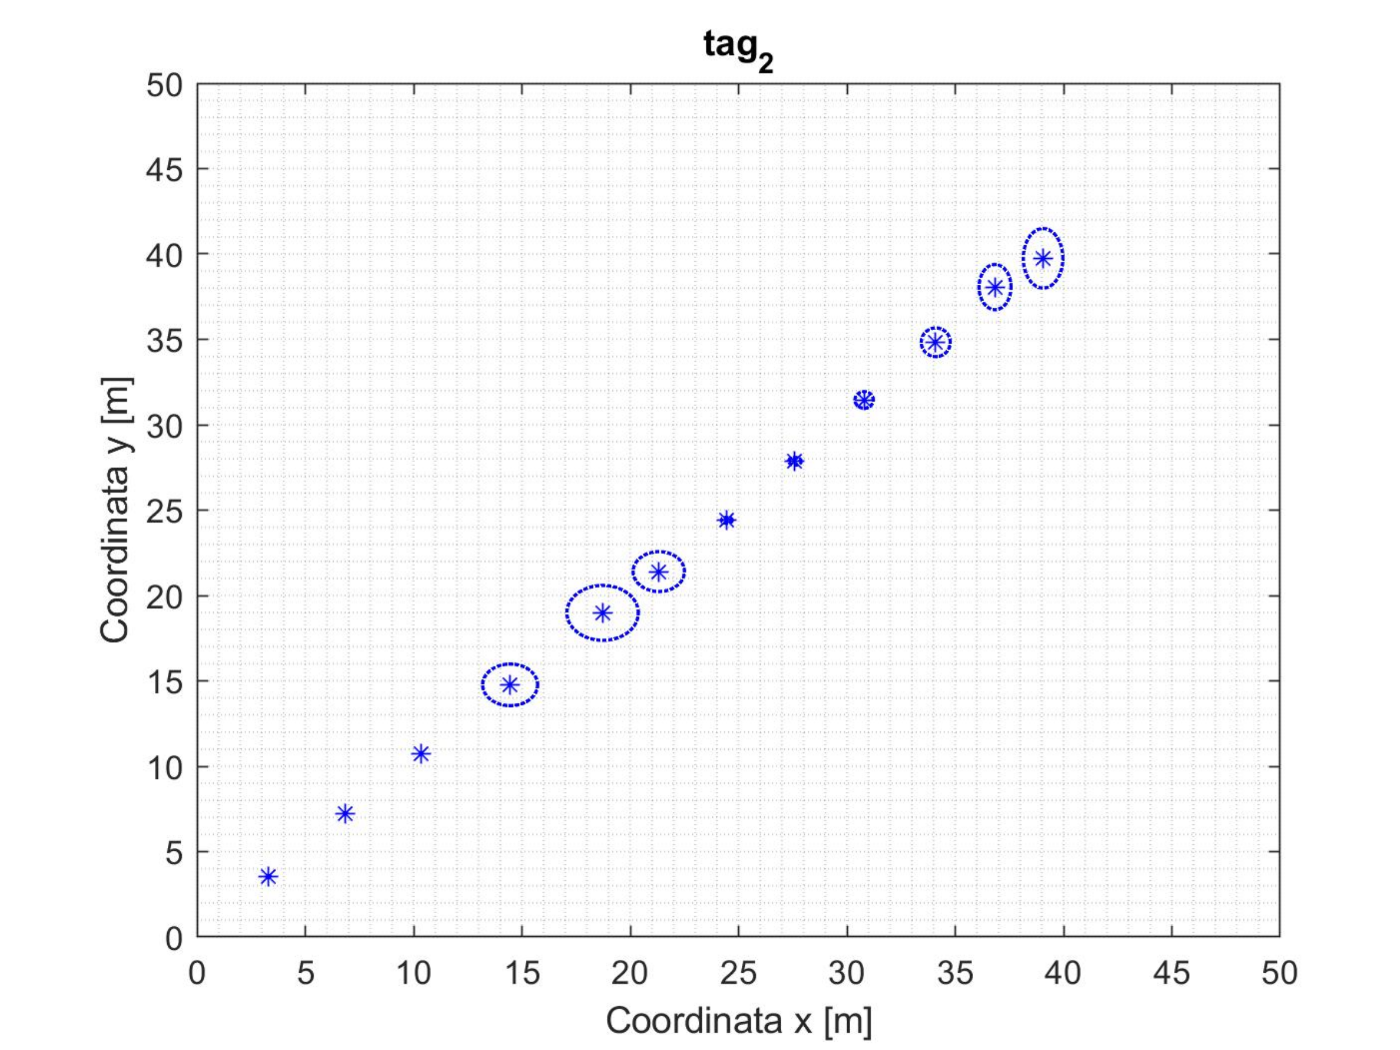
\includegraphics[scale=0.3]{EspOutPos20_2}
	 			\caption{\textbf{Figura 23:} posizione del tag 2 nel piano \textit{xy} durante l'esperimento sul positioning con distanza Ancora 0 - Ancora 1 = Ancora 0 - Ancora 2 = 20 m. Gli ellissi hanno semiassi corrispondenti alle deviazioni.\label{EspOutPos20_2}}
			\end{figure}

			\begin{figure}[H]
				\centering
				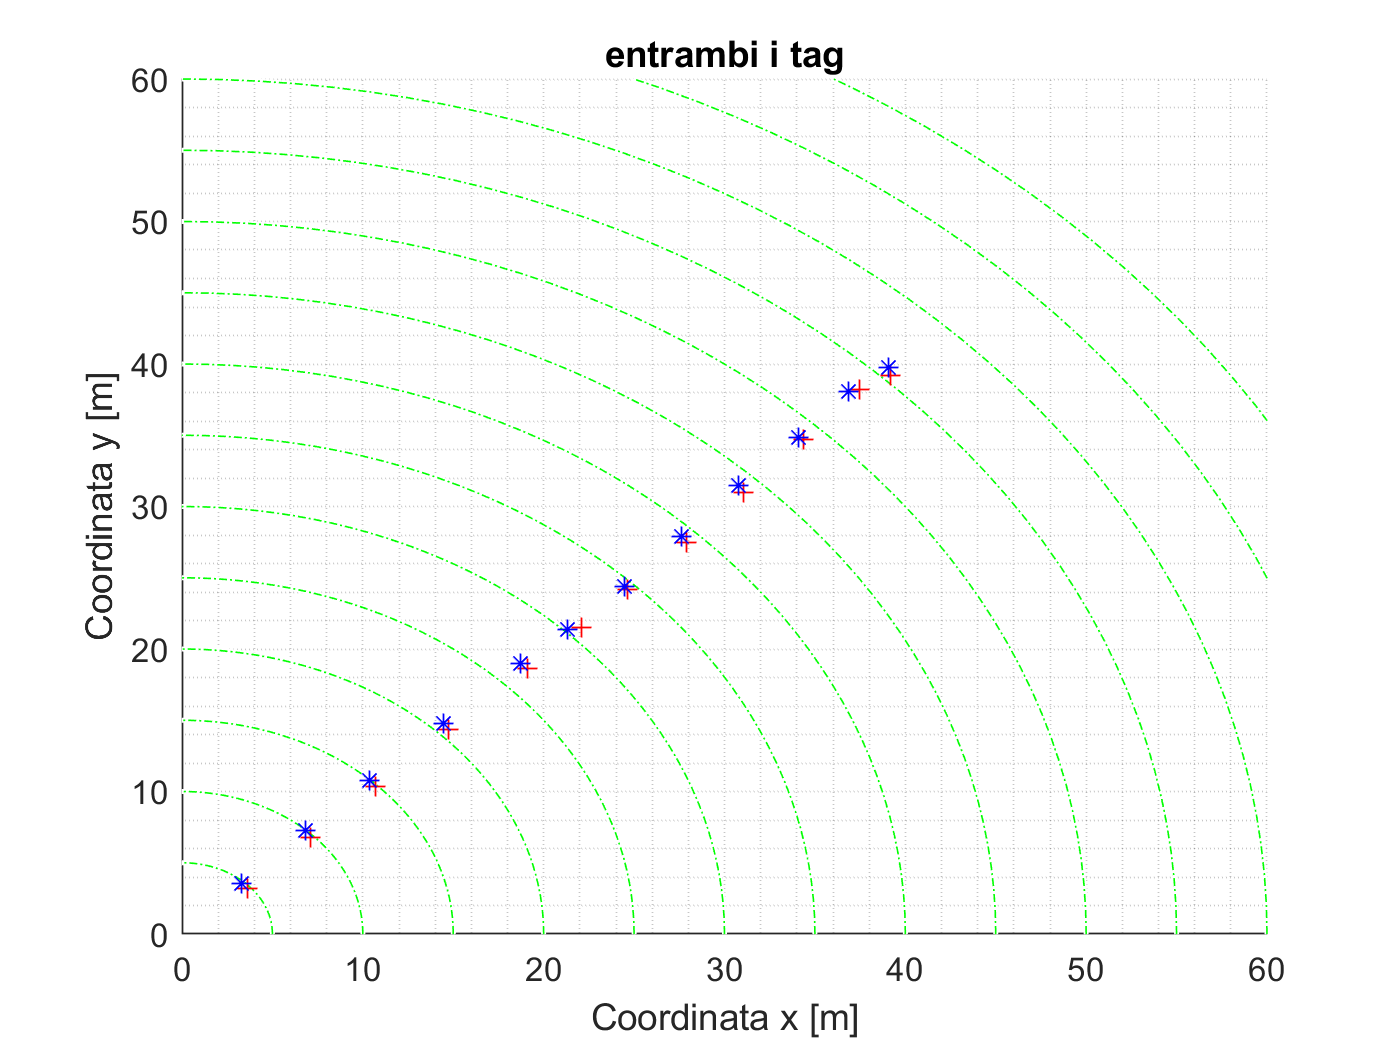
\includegraphics[scale=0.45]{EspOutPos20}
	 			\caption{\textbf{Figura 24:} rappresentazione di entrambi i tag nell'esperimento sul positioning con distanza Ancora 0 - Ancora 1 = Ancora 0 - Ancora 2 = 20 m. I cerchi sono concentrici e ogni circonferenza ha come raggio il set di distanze testate dall'Ancora 0.\label{EspOutPos20}}
			\end{figure}

			\begin{figure}[H]
				\centering
				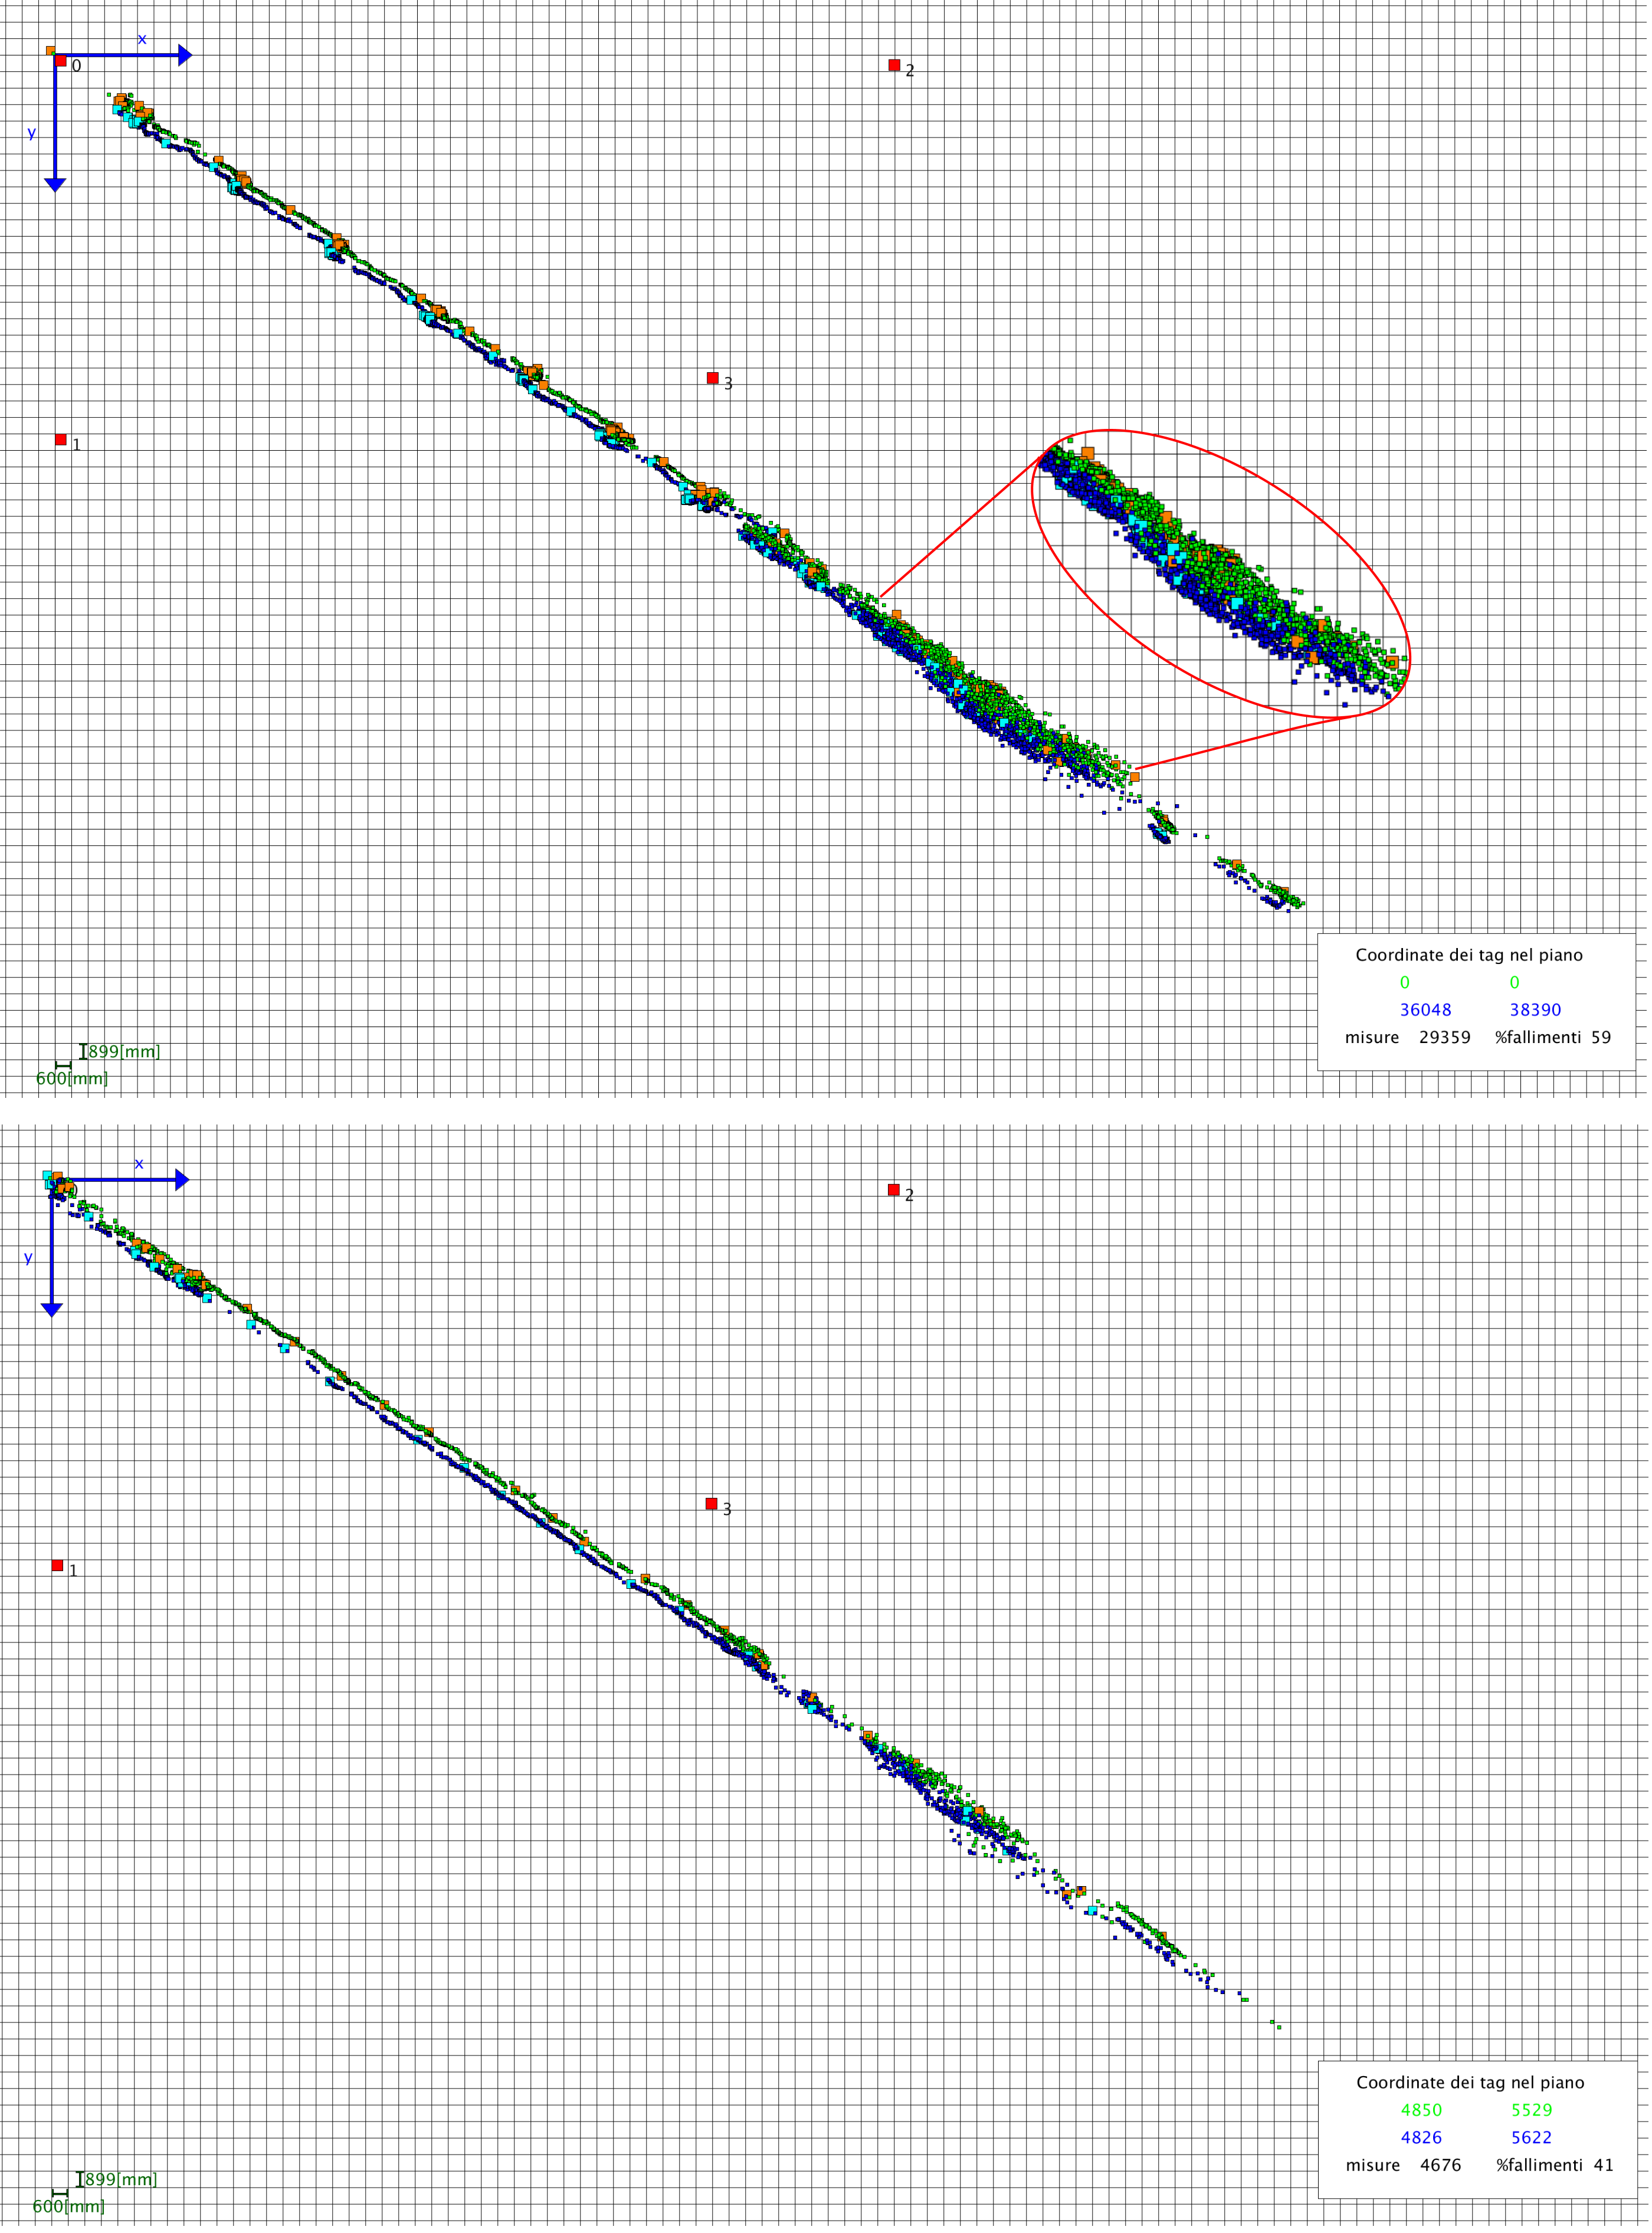
\includegraphics[scale=0.2]{EspOutPos2}
	 			\caption{\textbf{Figura 25:} esperimento positioning con distanza Ancora 0 - Ancora 1 = Ancora 0 - Ancora 2 = 30 m. Fase di allontanamento dall'Ancora 0 nella parte superiore dell'imagine, di avvicinamento nella parte inferiore\label{EspOutPos2}}
			\end{figure}

			\begin{figure}[H]
				\centering
				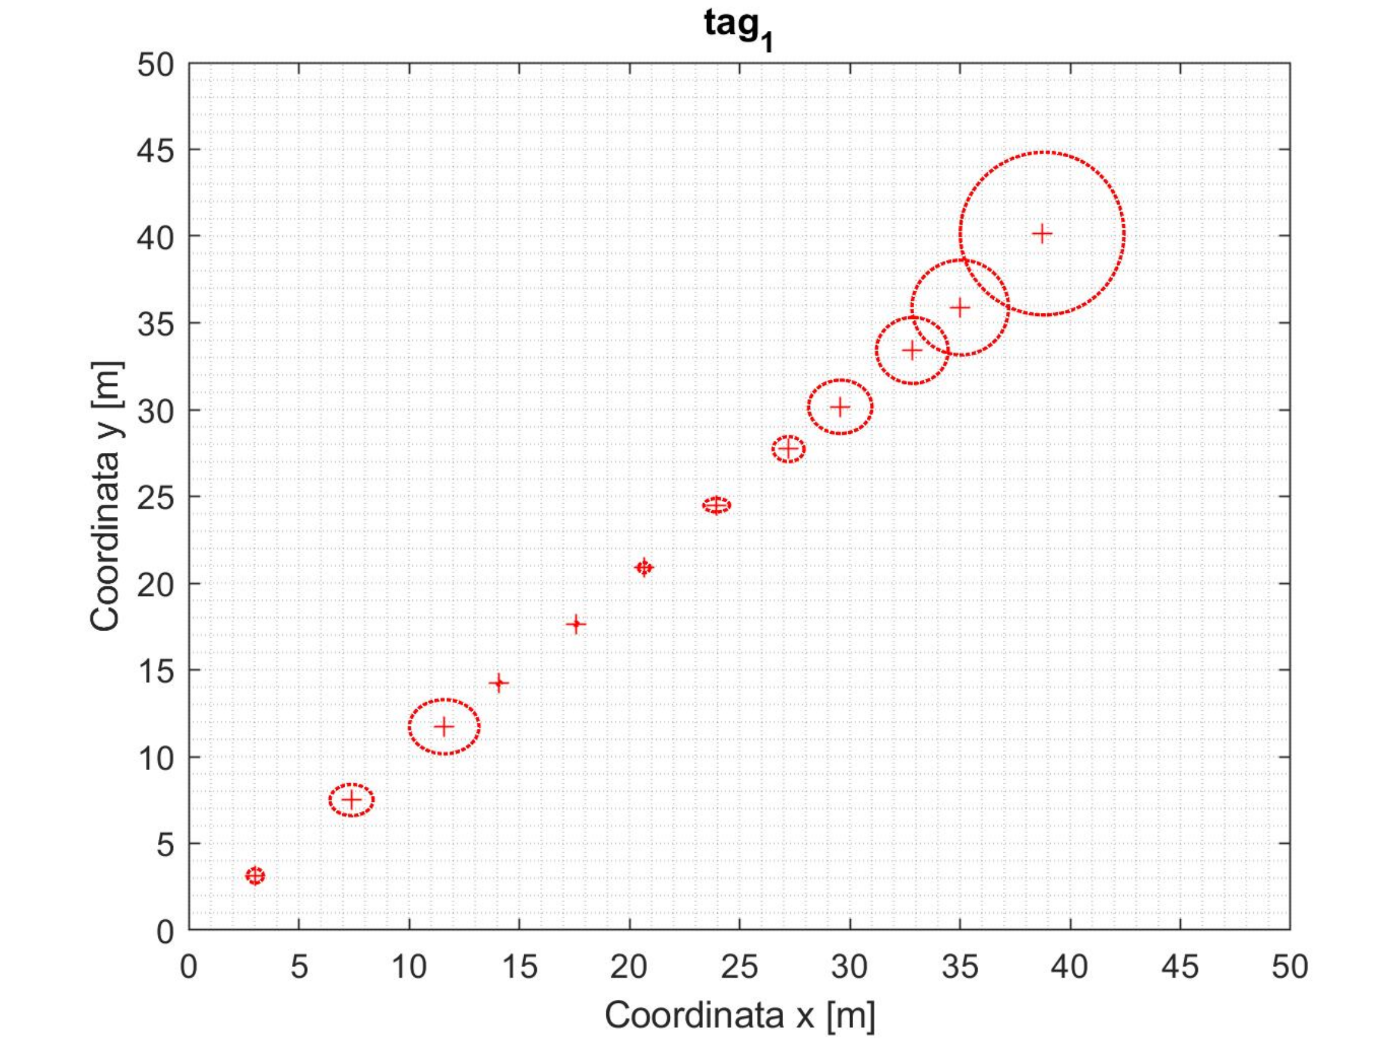
\includegraphics[scale=0.3]{EspOutPos30_1}
	 			\caption{\textbf{Figura 26:} posizione del tag 1 nel piano \textit{xy} durante l'esperimento sul positioning con distanza Ancora 0 - Ancora 1 = Ancora 0 - Ancora 2 = 30 m. Gli ellissi hanno semiassi corrispondenti alle deviazioni.\label{EspOutPos30_1}}
			\end{figure}

			\begin{figure}[H]
				\centering
				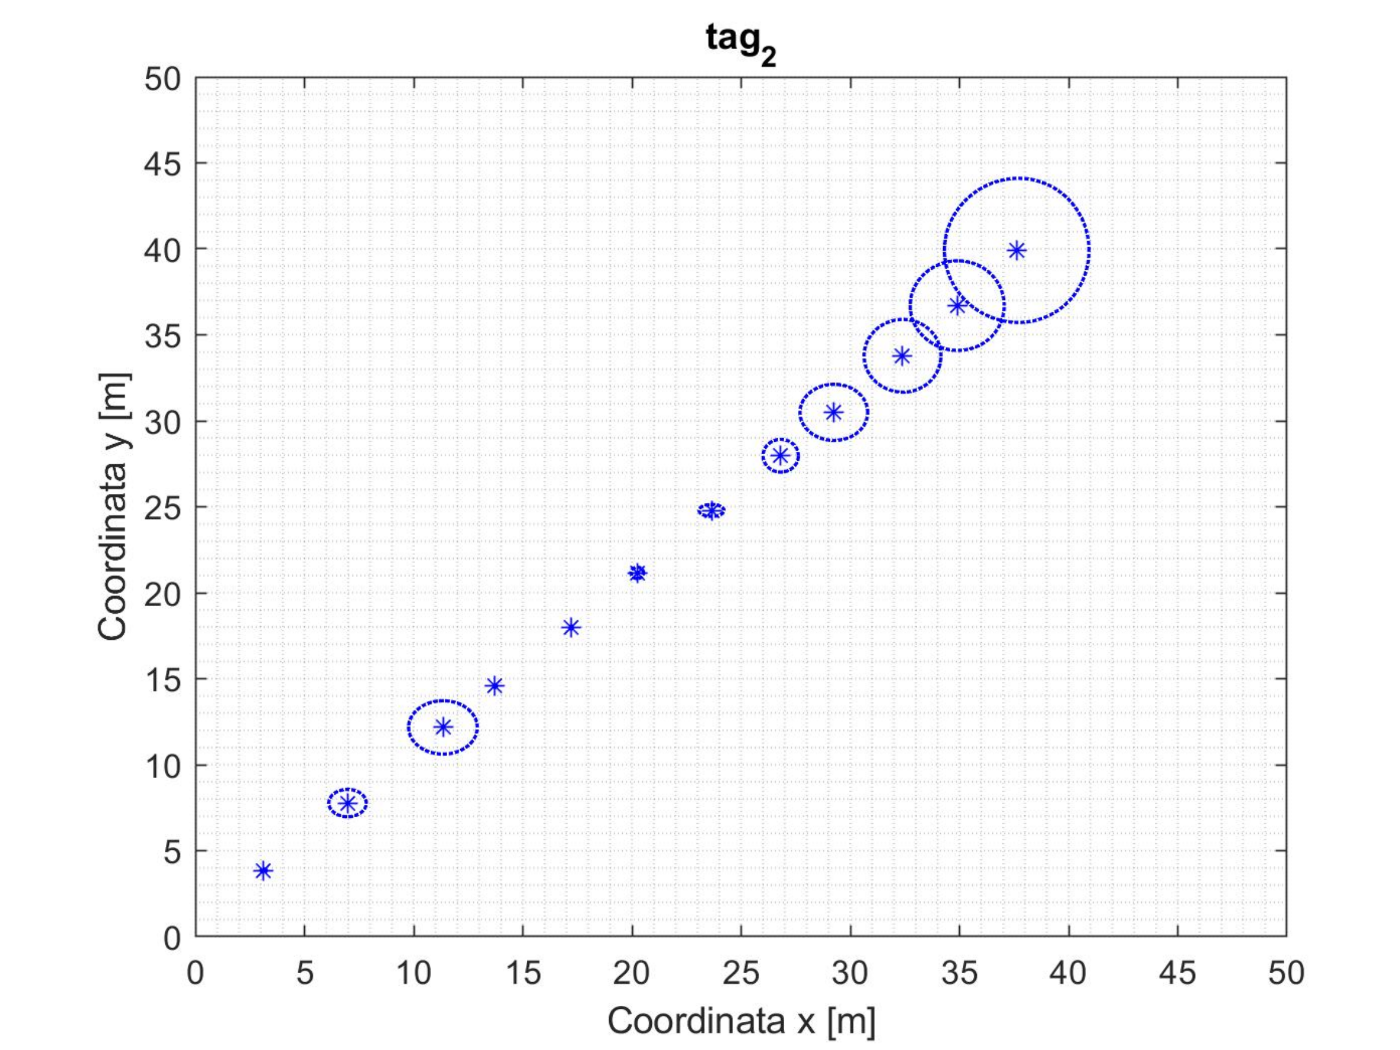
\includegraphics[scale=0.3]{EspOutPos30_2}
	 			\caption{\textbf{Figura 27:} posizione del tag 2 nel piano \textit{xy} durante l'esperimento sul positioning con distanza Ancora 0 - Ancora 1 = Ancora 0 - Ancora 2 = 30 m. Gli ellissi hanno semiassi corrispondenti alle deviazioni.\label{EspOutPos30_2}}
			\end{figure}

			\begin{figure}[H]
				\centering
				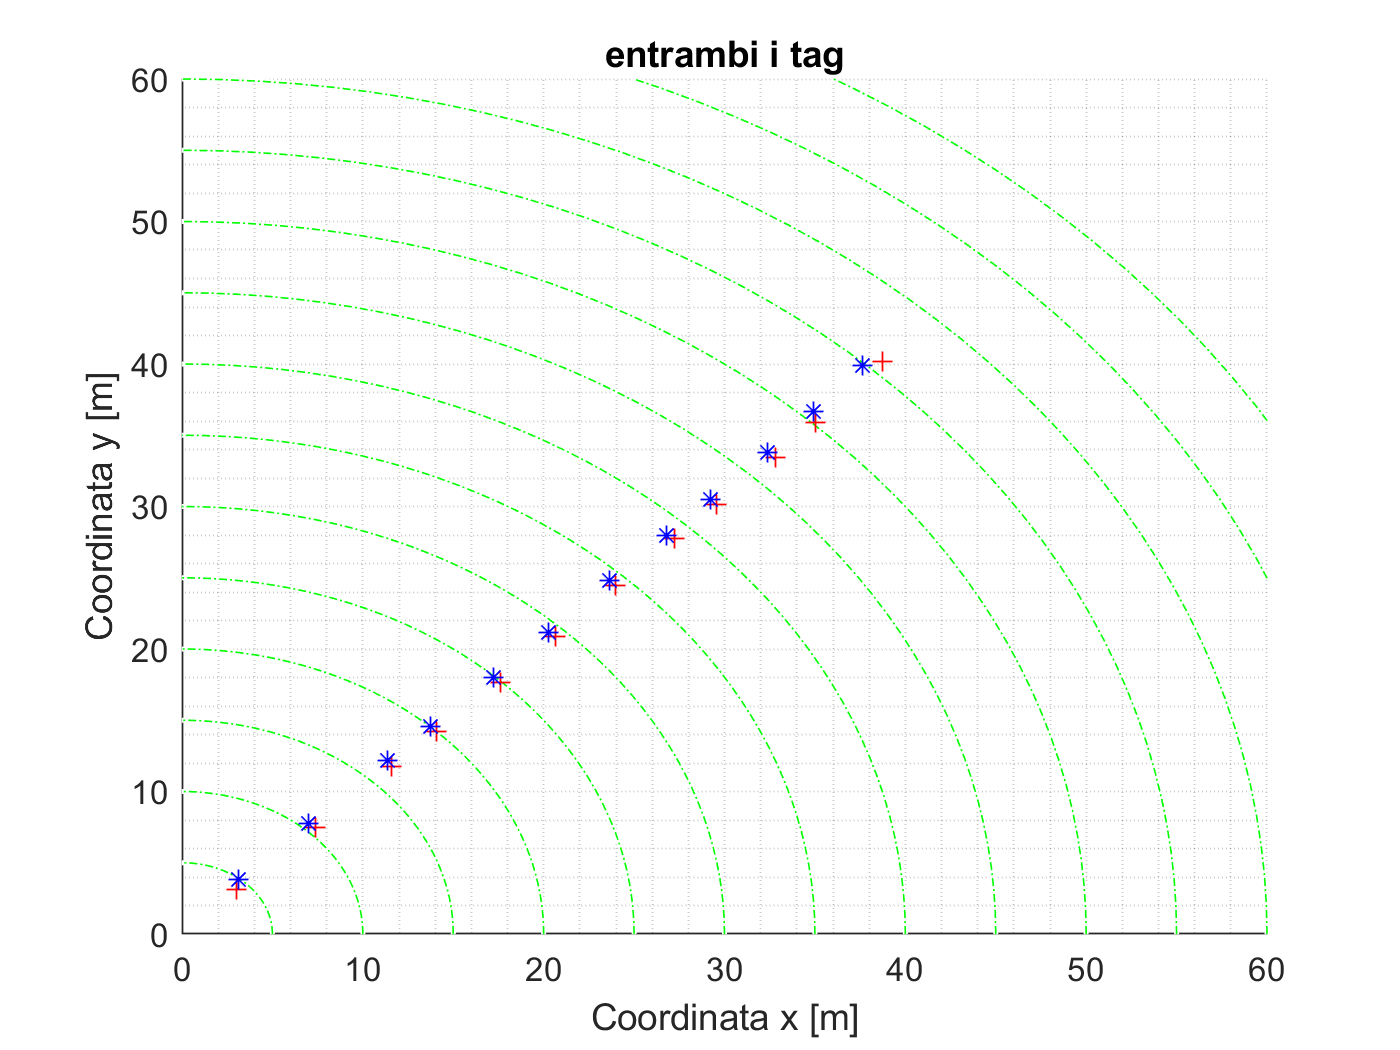
\includegraphics[scale=0.45]{EspOutPos30}
	 			\caption{\textbf{Figura 28:} rappresentazione di entrambi i tag nell'esperimento sul positioning con distanza Ancora 0 - Ancora 1 = Ancora 0 - Ancora 2 = 30 m. I cerchi sono concentrici e ogni circonferenza ha come raggio il set di distanze testate dall'Ancora 0.\label{EspOutPos30}}
			\end{figure}

			\begin{table}[H]
				\centering
\resizebox*{1.0\textwidth}{!}{
				\begin{tabular}{|c||c|c|c||c|c|c|c||}
					\hline
					\multicolumn{8}{|c|}{}\\
					\multicolumn{8}{|c|}{\textbf{\Large Tag 1}}\\
					\multicolumn{8}{|c|}{}\\
					\hline
					&\multicolumn{3}{|c||}{Coordinate [m]}&											\multicolumn{4}{|c||}{Distanze [m]}\\
					\hline
					Distanza&x& 				y& 				z& 										d0& 				d1&				d2&			d3\\
					ancora 0 [m]&&&&&&&\\
					\hline
					5&3.025$\pm$0.360&3.126$\pm$0.413&0.470$\pm$0.961&					4.337$\pm$0.450&27.652$\pm$0.947&27.422$\pm$0.290&24.785$\pm$0.425\\
					\hline
					10&7.3926$\pm$0.9781&7.495$\pm$0.889&0.411$\pm$0.531&			10.183$\pm$1.056&24.519$\pm$2.261&24.155$\pm$0.605&19.055$\pm$1.244\\
					\hline
					15&11.595$\pm$1.578&11.722$\pm$1.530&0.650$\pm$0.531&			16.100$\pm$1.956&22.455$\pm$2.853&22.031$\pm$0.474&13.201$\pm$2.132\\
					\hline
					20&14.091$\pm$0.094&14.227$\pm$0.101&0.783$\pm$0.497&			19.785$\pm$0.066&22.879$\pm$6.548&21.439$\pm$0.040&10.115$\pm$0.051\\
					\hline
					25&17.587$\pm$0.077&17.649$\pm$0.096&0.526$\pm$0.495&			24.765$\pm$0.076&22.579$\pm$5.570&21.520$\pm$0.043&6.104$\pm$0.059\\
					\hline
					30&20.669$\pm$0.262&20.885$\pm$0.275&0.796$\pm$0.575&			29.766$\pm$0.321&23.154$\pm$3.531&22.786$\pm$0.134&4.695$\pm$0.045\\
					\hline
					35&23.958$\pm$0.585&24.488$\pm$0.354&1.844$\pm$1.866&			34.893$\pm$0.464&28.912$\pm$11.227&25.155$\pm$0.161&7.42$\pm$0.343\\
					\hline
					40&27.220$\pm$0.704&27.722$\pm$0.64&1.037$\pm$5.034&				39.907$\pm$0.034&28.436$\pm$4.513&28.207$\pm$0.039&11.801$\pm$0.034\\
					\hline
					45&29.568$\pm$1.437&30.159$\pm$1.338&4.166$\pm$8.234&			44.713$\pm$0.050&31.089$\pm$0.070&31.491$\pm$0.043&16.284$\pm$0.052\\
					\hline
					50&32.838$\pm$1.626&33.408$\pm$1.597&5.310$\pm$9.862&			49.702$\pm$0.073&34.907$\pm$0.073&35.256$\pm$0.066&21.074$\pm$0.062\\
					\hline
					55&35.011$\pm$2.194&35.881$\pm$2.237&4.687$\pm$13.067&			54.022$\pm$0.722&38.241$\pm$0.0581&38.853$\pm$0.603&25.351$\pm$0.709\\
					\hline
					60&38.727$\pm$3.716&40.145$\pm$3.657&8.221$\pm$17.400&			61.734$\pm$2.916&44.767$\pm$2.669&45.679$\pm$2.456&33.057$\pm$2.842\\
					\hline
					\hline
					\multicolumn{8}{|c|}{}\\
					\multicolumn{8}{|c|}{\textbf{\Large Tag 2}}\\
					\multicolumn{8}{|c|}{}\\
					\hline
					&\multicolumn{3}{|c||}{Coordinate [m]}&											\multicolumn{4}{|c||}{Distanze [m]}\\
					\hline
					Distanza&x& 				y& 				z& 														d0& 				d1&				d2&			d3\\
					ancora 0 [m]&&&&&&&\\
					\hline
					5&3.130$\pm$0.122&3.853$\pm$0.100&0.183$\pm$0.100&    			4.418$\pm$0.448&27.183$\pm$0.967&27.700$\pm$0.292&24.859$\pm$0.4660\\
					\hline
				    10&6.970$\pm$0.857&7.769$\pm$0.788&0.420$\pm$0.252&   			10.205$\pm$1.365&23.967$\pm$1.349&24.532$\pm$0.569&19.182$\pm$1.2310\\
					\hline
				   15&11.341$\pm$1.574&12.168$\pm$1.522&0.374$\pm$0.475&  			16.093$\pm$1.847&21.745$\pm$1.002&22.470$\pm$0.478&13.383$\pm$2.0370\\
					\hline
				   20&13.724$\pm$0.074&14.571$\pm$0.077&0.264$\pm$0.513&   		19.772$\pm$0.037&21.121$\pm$1.842&21.878$\pm$0.056&10.387$\pm$0.0360\\
					\hline
				   25&17.205$\pm$0.072&17.978$\pm$0.085&0.592$\pm$0.351&   		24.770$\pm$0.066&21.210$\pm$1.287&21.961$\pm$0.036&6.476$\pm$0.0590\\
					\hline
				   30&20.240$\pm$0.287&21.156$\pm$0.311&0.774$\pm$0.563&   		29.742$\pm$0.333&22.402$\pm$1.293&23.242$\pm$0.138&5.187$\pm$0.0480\\
					\hline
				   35&23.641$\pm$0.572&24.786$\pm$0.315&1.607$\pm$1.956&   		34.829$\pm$0.398&24.520$\pm$1.626&25.505$\pm$0.118&7.643$\pm$0.2690\\
					\hline
				   40&26.812$\pm$0.811&27.968$\pm$0.849&3.938$\pm$4.102&   		39.885$\pm$0.062&27.599$\pm$0.104&28.618$\pm$0.030&11.968$\pm$0.0340\\
					\hline
				   45&29.244$\pm$1.551&30.490$\pm$1.424&6.618$\pm$6.150&   		44.620$\pm$0.070&30.858$\pm$0.186&31.802$\pm$0.072&16.319$\pm$0.0770\\
					\hline
				   50&32.390$\pm$1.759&33.780$\pm$1.786&5.838$\pm$9.701&   		49.734$\pm$0.071&34.555$\pm$0.071&35.669$\pm$0.096&21.204$\pm$0.0820\\
					\hline
				   55&34.896$\pm$2.154&36.699$\pm$2.136&4.950$\pm$11.897&   		53.933$\pm$0.710&37.895$\pm$0.611&39.103$\pm$0.585&25.343$\pm$0.7020\\
					\hline
				   60&37.621$\pm$3.310&39.910$\pm$3.320&10.792$\pm$16.228&   	61.658$\pm$2.806&44.424$\pm$2.597&45.876$\pm$2.307&33.038$\pm$2.7330\\
					\hline
				\end{tabular}
}
				\caption{\textbf{Tabella 14:} esperimento positioning con distanza Ancora 0 - Ancora 1 = Ancora 0 - Ancora 2 = 30 m\label{EspOut30}}
			\end{table}

\begin{table}[H]
				\centering
				\begin{tabular}{|c||c|c||c|c|}
					\hline
					\multicolumn{5}{|c|}{}\\
					\multicolumn{5}{|c|}{\textbf{\Large Distanze dall'Ancora 0}}\\
					\multicolumn{5}{|c|}{}\\
					\hline
					\multirow{2}{*}{Reale}&\multicolumn{2}{|c||}{Tag 1}&	\multicolumn{2}{|c|}{Tag2}\\
					\cline{2-5}
					&$\sqrt{(x^2+y^2)}$& d0& 		$\sqrt{(x^2+y^2)}$& d0\\
					\hline
				    5&4.826&    	  4.761&     4.833&    4.791\\
					\hline
    				10&9.838&     9.862&   	  9.973&    9.987\\
					\hline
   					15&14.892&   14.916&   14.913&   14.942\\
					\hline
   					20&20.592&   20.653&   20.664&   20.669\\
					\hline
   					25&26.671&   26.751&   26.662&   26.642\\
					\hline
   					30&30.818&   30.719&   30.206&   30.615\\
					\hline
  					35&34.527&   35.026&   34.550&   34.965\\
					\hline
   					40&39.173&   39.846&   39.217&   39.883\\
					\hline
   					45&43.857&   44.933&   44.016&   44.886\\
					\hline 
 					50&48.862&   49.814&   48.742&   49.674\\
					\hline
   					55&53.525&   54.614&   52.968&   54.584\\
					\hline
   					60&55.409&   59.182&   55.723&   59.249\\
					\hline
				\end{tabular}
				\caption{\textbf{Tabella 15:} Confronto tra ranging e distanza planare rispetto all'Ancora 0; riferiti all'esperimento positioning con distanza Ancora 0 - Ancora 1 = Ancora 0 - Ancora 2 = 30 m. \label{EspOut30}}
			\end{table}

			Sono stati analizzati i dati relativi alla frequenza di update rate, i cui risultati vengono riportati in \textbf{\tablename~\ref{EspOutFreq}}. Da essi si evince sostanzialmente come lungo tutto il percorso la frequenza rimanga invariata e come, anche variando le distanze relative tra le ancore, tale grandezza non 						venga granchè modificata.
			\begin{table}[H]
					\centering
					\begin{tabular}{|c|c||c|}
						\hline
						\multicolumn{3}{|c|}{}\\
						\multicolumn{3}{|c|}{\textbf{\Large Frequenze}}\\
						\multicolumn{3}{|c|}{}\\
						\hline
						Distanza&			\multirow{2}{*}{20 m}&  \multirow{2}{*}{30 m}\\
						ancora 0 [m]&&\\
						\hline
   						5&		    							37&		    39\\
						\hline
    					10&										37&    		39\\
						\hline
    					15&										37&		    39\\
						\hline
   						20&										37&    		40\\
						\hline
    					25&										37&    		39\\
						\hline
    					30&										37&    		38\\
						\hline
    					35&										37&    		40\\
						\hline
    					40&										37&    		38\\
						\hline
    					45&										36&    		38\\
						\hline
    					50&										37&    		37\\
						\hline
    					55&										39&    		38\\
						\hline
    					60&										36&    		35\\
						\hline
					\end{tabular}
					\caption{\textbf{Tabella 16:} esperimento positioning confronto frequenza: nella colonna di sinistra sono riportate le frequenze a cui il loop lavora con distanza tra le ancore pari a $20 m$, in quella di destra per una distanza di $30m$ \label{EspOutFreq}}
				\end{table}

				Vengono infine presi in considerazione i fallimenti dell'algoritmo del positioning. In questo caso si nota come il numero di fallimenti risulti tendenzialmente elevato. Esso sembra fortemente connesso alle distanze dalle ancore. Infatti nell'area centrale al quadrato formato i fallimenti sono inferiori e vanno via 						via aumentando alle estremità e al di fuori del quadrato stesso. Non verrà quindi effettivamente aggiornata la misura in corrispondenza di ogni loop di Arduino.
				\begin{table}[H]
					\centering
					\begin{tabular}{|c|c|c||c|c|}
						\hline
						\multicolumn{5}{|c|}{}\\
						\multicolumn{5}{|c|}{\textbf{\Large Fallimenti}}\\
						\multicolumn{5}{|c|}{}\\
						\hline
						Distanza&			\multicolumn{2}{|c||}{20 m}&  \multicolumn{2}{|c|}{30 m}\\
						ancora 0 [m]&\multicolumn{2}{|c||}{}&\multicolumn{2}{|c|}{}\\
						\hline
   						5&									26.7&   75.4&   											31.9&   69.6\\
						\hline
   						10&									26.6&   30.0&   											40.4&   27.9\\
						\hline
   						15&									31.2&   36.1&  											39.5&   36.8\\
						\hline
   						20&									34.6&   64.2&   											48.7&   50.8\\
						\hline
   						25&									35.4&   53.5&   											37.7&   45.2\\
						\hline
   						30&									41.0&   47.5&   											53.9&   45.8\\
						\hline
   						35&									41.3&   79.5&   											50.5&   71.7\\
						\hline
   						40&									53.2&   60.0&   											52.3&   63.0\\
						\hline
   						45&									46.4&   74.2&   											65.0&   83.0\\
						\hline
   						50&									54.2&   52.7&   											76.8&   44.4\\
						\hline
   						55&									84.8&   64.8&   											96.9&   80.5\\
						\hline
   						60&									57.9&   42.6&   											83.3&   52.2\\
						\hline
					\end{tabular}
				\caption{\textbf{Tabella 17:} esperimento positioning confronto fallimenti: nelle colonne di sinistra sono riportate le percentuali di fallimento del tag 1 nei due esperimenti; in quelle di destra del tag 2\label{EspOutFall}}
			\end{table}

		\end{subsection}

		\begin{subsection}{Conclusioni sugli esperimenti outdoor}
				
				In termini di distanza massima di comunicazione tra le antenne, si nota un netto miglioramento all’aumentare del bitrate. In particolare dall’esperimento sul ranging, si evidenzia come, settando il \textbf{bitrate} a $6810 kbit/s$, la comunicazione risulti efficace fino a circa $60m$. Quando il \textbf{bitrate} è 					invece pari a $110 kbit/s$, la comunicazione tra 2 antenne fallisce già per distanze superiori a $30m$. Risultato in generale intermedio tra i due si ottiene per bitrate pari a $850kbit/s$.
				La distanza massima di comunicazione viene inoltre fortemente influenzata dal valore di \textbf{gain}. In particolare, settando il massimo \textbf{gain} a 33, si osserva quanto ci si aspettava. Infatti, come anche la documentazione Pozyx afferma, un aumento di  tale parametro determina un notevole 								incremento della distanza di comunicazione.\\
				Dunque per ottenere ampie aree coperte dal segnale delle antenne, è necessario impostare il \textbf{gain} e il \textbf{bitrate} al loro massimo valore. I parametri ottimi riscontrati dagli esperimenti indoor, risultano comprovati anche all'esterno.

		\end{subsection}

	\end{section}

	\begin{section}{Affidabilità del sistema POZYX}

		Dopo gli scarsi risultati rilevati dall’esperimento outdoor in termini di fallimenti, è stato effettuato un ulteriore esperimento indoor. Il test si è posto l’obiettivo di interpretare l’andamento dei ranging nel tempo, investigando sulle cause di una mancata convergenza dell’algoritmo di positioning.
		Infatti, noi non siamo a conoscenza sia del modo in cui tale algoritmo viene implementato sia di quali condizioni di lavoro possono danneggiare la comunicazione wireless. 
		Rispetto al sistema originale di localizzazione Pozyx, in questo progetto sono state apportate delle modifiche hardware e software che permettono la comunicazione I$^2$C con due tag, gestita direttamente dagli sketch Arduino. Con questo test cerchiamo di capire se questo modo di lavorare con due tag 							simultaneamente potesse non essere supportato e fosse il responsabile delle prestazioni poco soddisfacenti.\\

		Durante quest’ultimo esperimento è stato realizzato appositamente un nuovo sketch Arduino. Esso, ogni 250 campioni, avvia la comunicazione del tag o  dei tag  specificandone l’indirizzo I$^2$C. Cioè, per  primi 250 campioni viene inizializzato il tag con indirizzo I$^2$C $0X4A$ che deve eseguire le seguenti 					operazioni: esso richiede alle ancore il doPositioning; sia nel caso in cui questa operazione avesse un esito positivo (status =1) che nel caso in cui status fosse pari a 0, viene eseguito \textit{GetDeviceRangeInfo}. Quindi, in ogni caso i ranging vengono aggiornati. Però, il caso in cui status è pari a 0, è rilevato come 		un errore e le coordinate vengono settate a 0. Infatti, in questo caso la trilaterazione non è avvenuta e le coordinate del tag non sono state aggiornate. Alcune volte, si è però riscontrato che, nonostante l’algoritmo di doPositioning avesse avuto esito positivo (status =1) e quindi i ranging fossero stati definiti, le 				coordinate venissero settate tutte e tre al valore nullo. Per tener conto di questo possibile caso è stata definita la variabile "\textit{error}", che viene posta a 1 nel momento in cui le coordinate sono nulle.\\ 
		Per 250 campioni successivi viene inizializzata la comunicazione I$^2$C con il tag avente indirizzo $0X4B$ che esegue le stesse istruzioni descritte in precedenza.\\
		Per gli ultimi 500 campioni, la comunicazione avviene con entrambi i tag. Ma, l’inizializzazione dei tag avviene in ordine differente, Ovvero, di questi 500 campioni, nei primi 250 parte prima la comunicazione con $0x4A$ e poi con $0x4B$; viceversa negli ultimi 250. 
		Sono stati eseguiti 6 cicli da 1000 campioni shiftando in questo modo tra gli indirizzi.
		Nel primo, terzo, quinto ciclo eravamo fermi nella stessa posizione mentre in quelli intermedi ci spostavamo per raggiungere un’altra postazione.\\

		In \textbf{\figurename~\ref{ConfDist}} sono riportati i ranging rilevati da entrambi i tag. In linea continua, quelli relativi al primo tag e in linea tratteggiata quelli relativi al secondo.
		In basso, sono presenti 4 onde quadre. Le prime due si riferiscono al primo tag e quelle tratteggiate al secondo tag.
		In particolare, le linee blu si riferiscono all’errore e le rosse allo status.
		Quando, per ogni tag, entrambe le linee dei controlli sono settate a 1, è avvenuta la convergenza dell’algoritmo di \textit{doPositioning} e  non  si sono riscontrati errori, ovvero le coordinate assumono valori diversi da zero. Quando status è basso, vuol dire che l’algoritmo non è convergente. Dunque, affinchè non 			ci fosse alcuna incongruenza, anche l’errore sarebbe dovuto essere basso. 
		Non sempre questo accade. Infatti, svariate volte status è alto ma si rilevano errori. 
		In questi casi, focalizzandoci sui singoli ranging, essi sembrano non essere affetti da un eccessivo disturbo. 
		È ciò che succede proprio nell’intervallo di campioni [3500, 4000].
		Dai risultati si evince però che la comunicazione I$^2$C si avvia in modo corretto inizializzando ogni volta il tag definito.\\
		\begin{figure}[H]
			\centering
			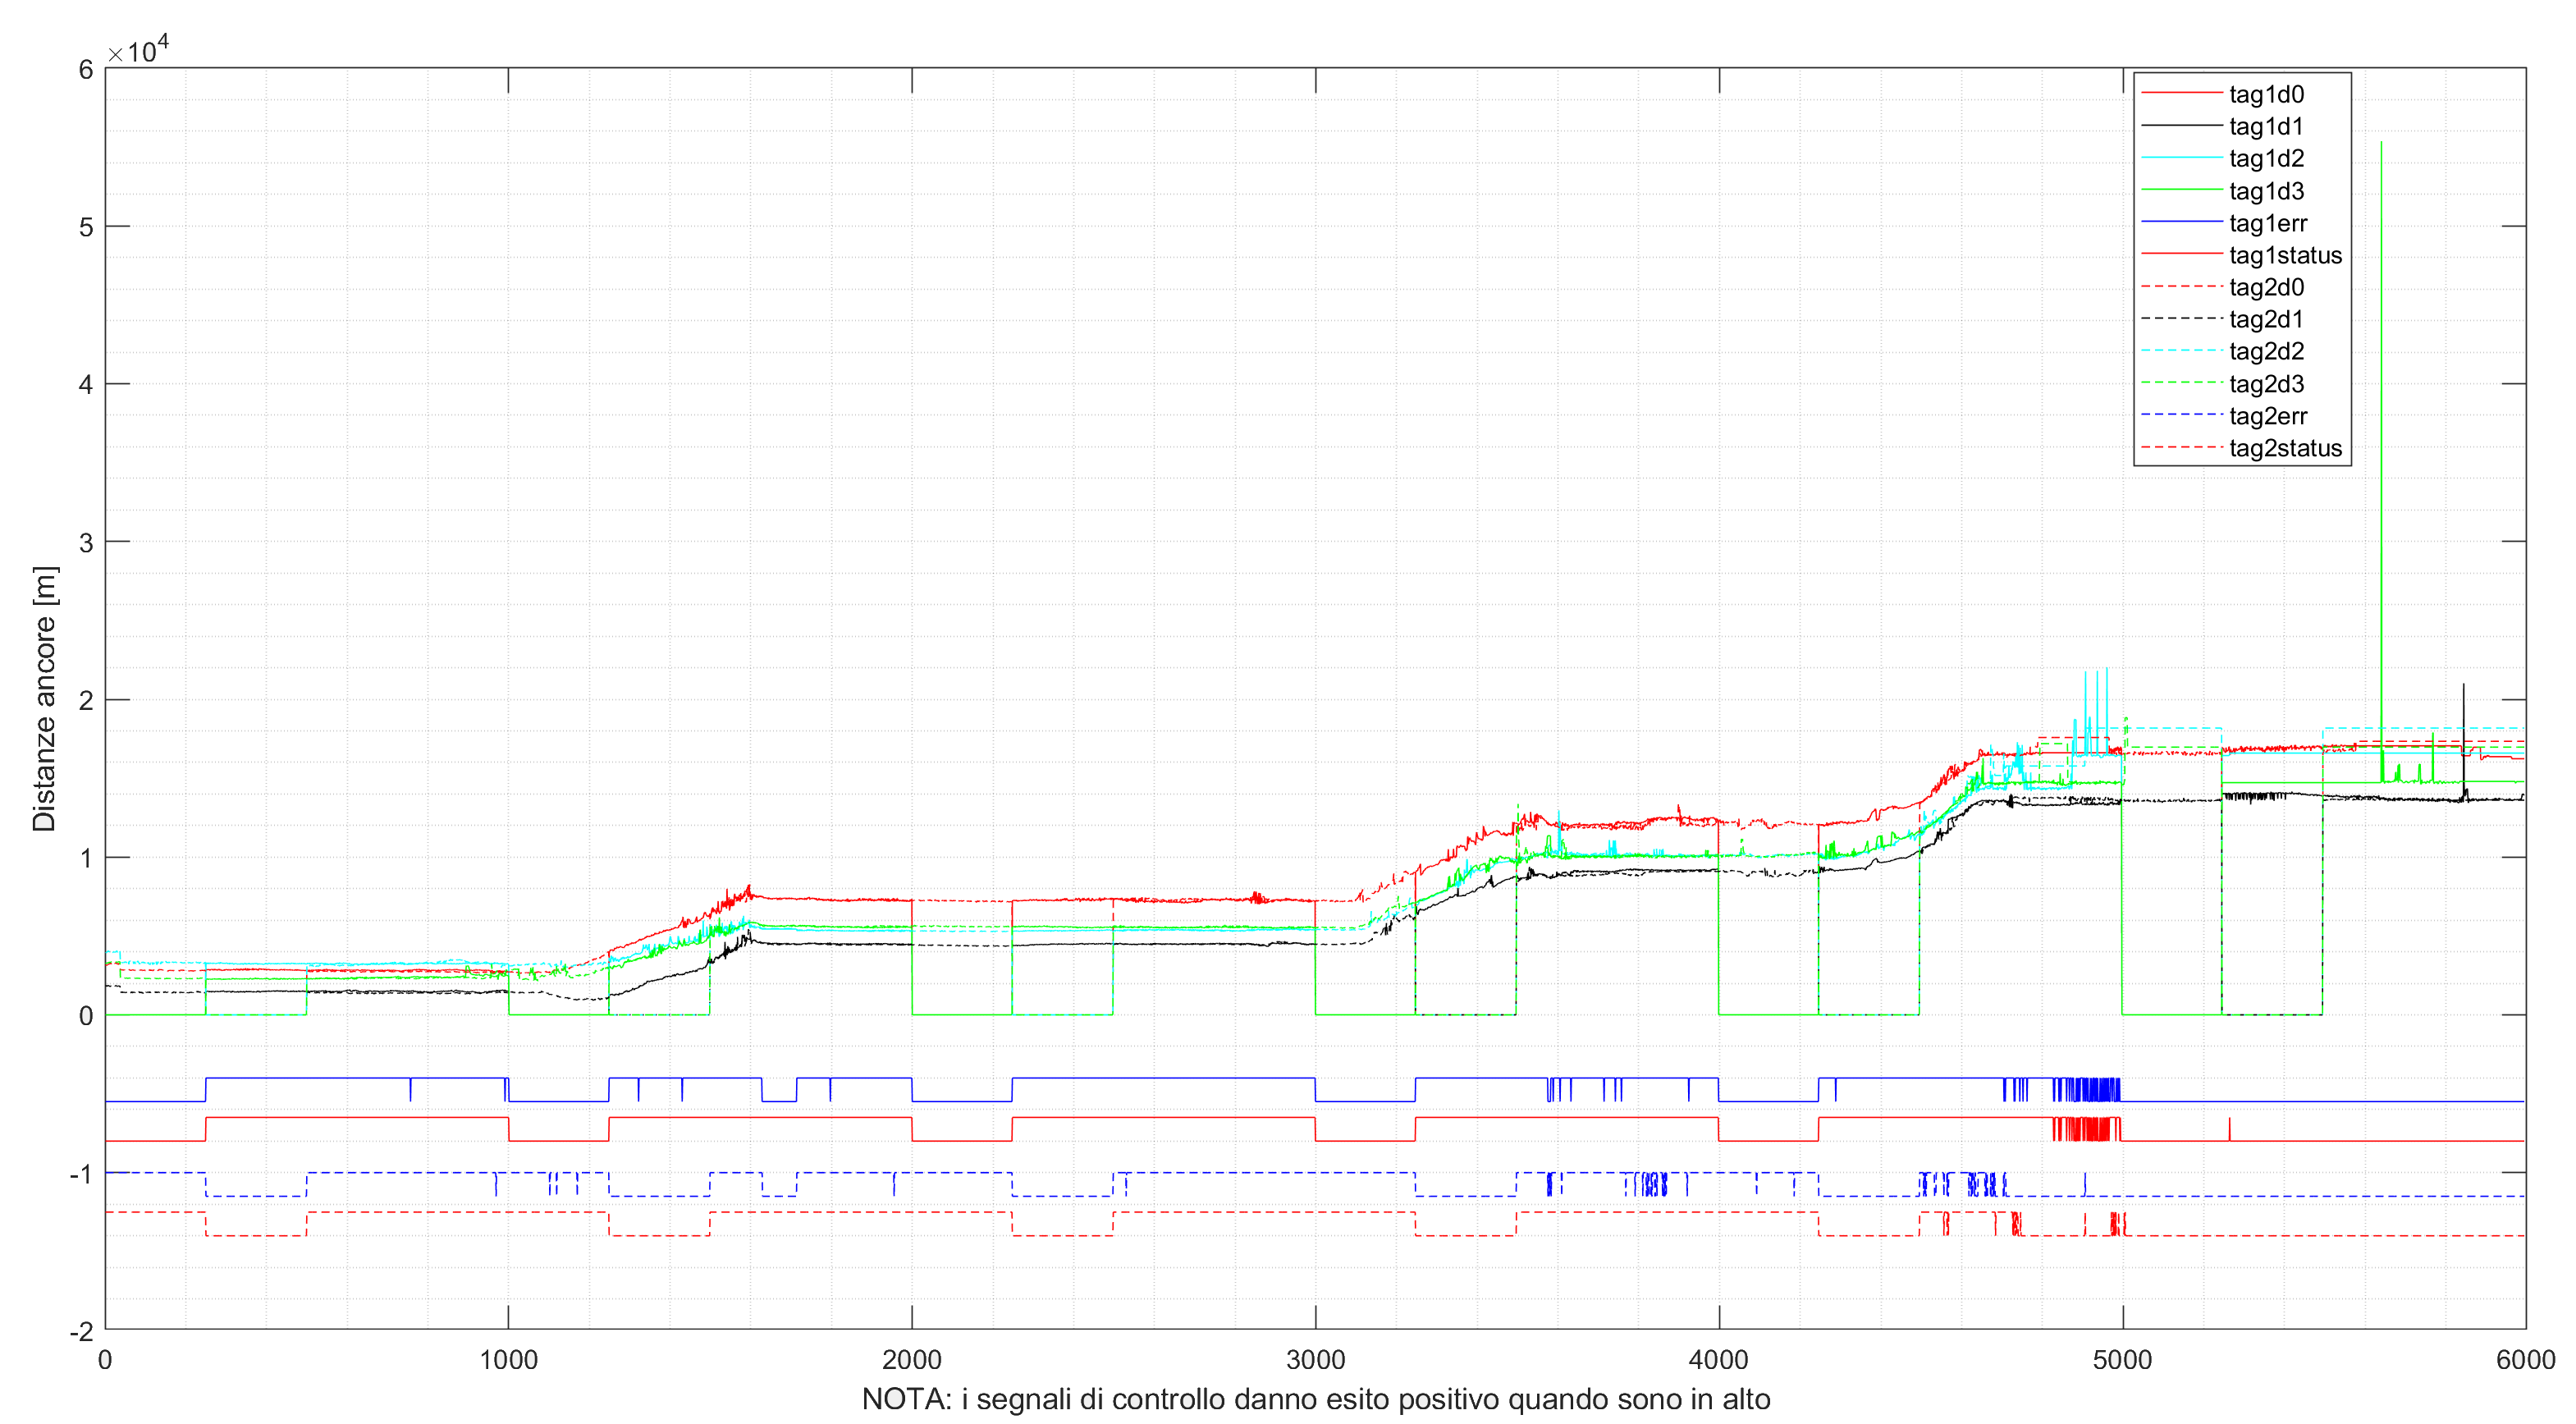
\includegraphics[scale=0.17]{ConfDist}
			\caption{\textbf{Figura 29:} confronto delle distanze ottenute con status e errori registrati\label{ConfDist}}
		\end{figure} 
		Sono anche riportate due figure che confrontano il ranging dall’ancora 0 con la norma ricavata dalle coordinate planari x e y sia per il tag 1 (\textbf{\figurename~\ref{PosRangTag1}}) che per il tag2 (\textbf{\figurename~\ref{PosRangTag2}}). 
		Si nota subito che il gli errori sono più frequenti man mano che la distanza dall’ancora 0 aumenta. In particolare, si osserva che, per un intervallo di campioni in cui entrambi i tag erano attivi, le distanze siano traslate rispetto al valore ottenuto dalla norma.\\
		\begin{figure}[H]
			\centering
			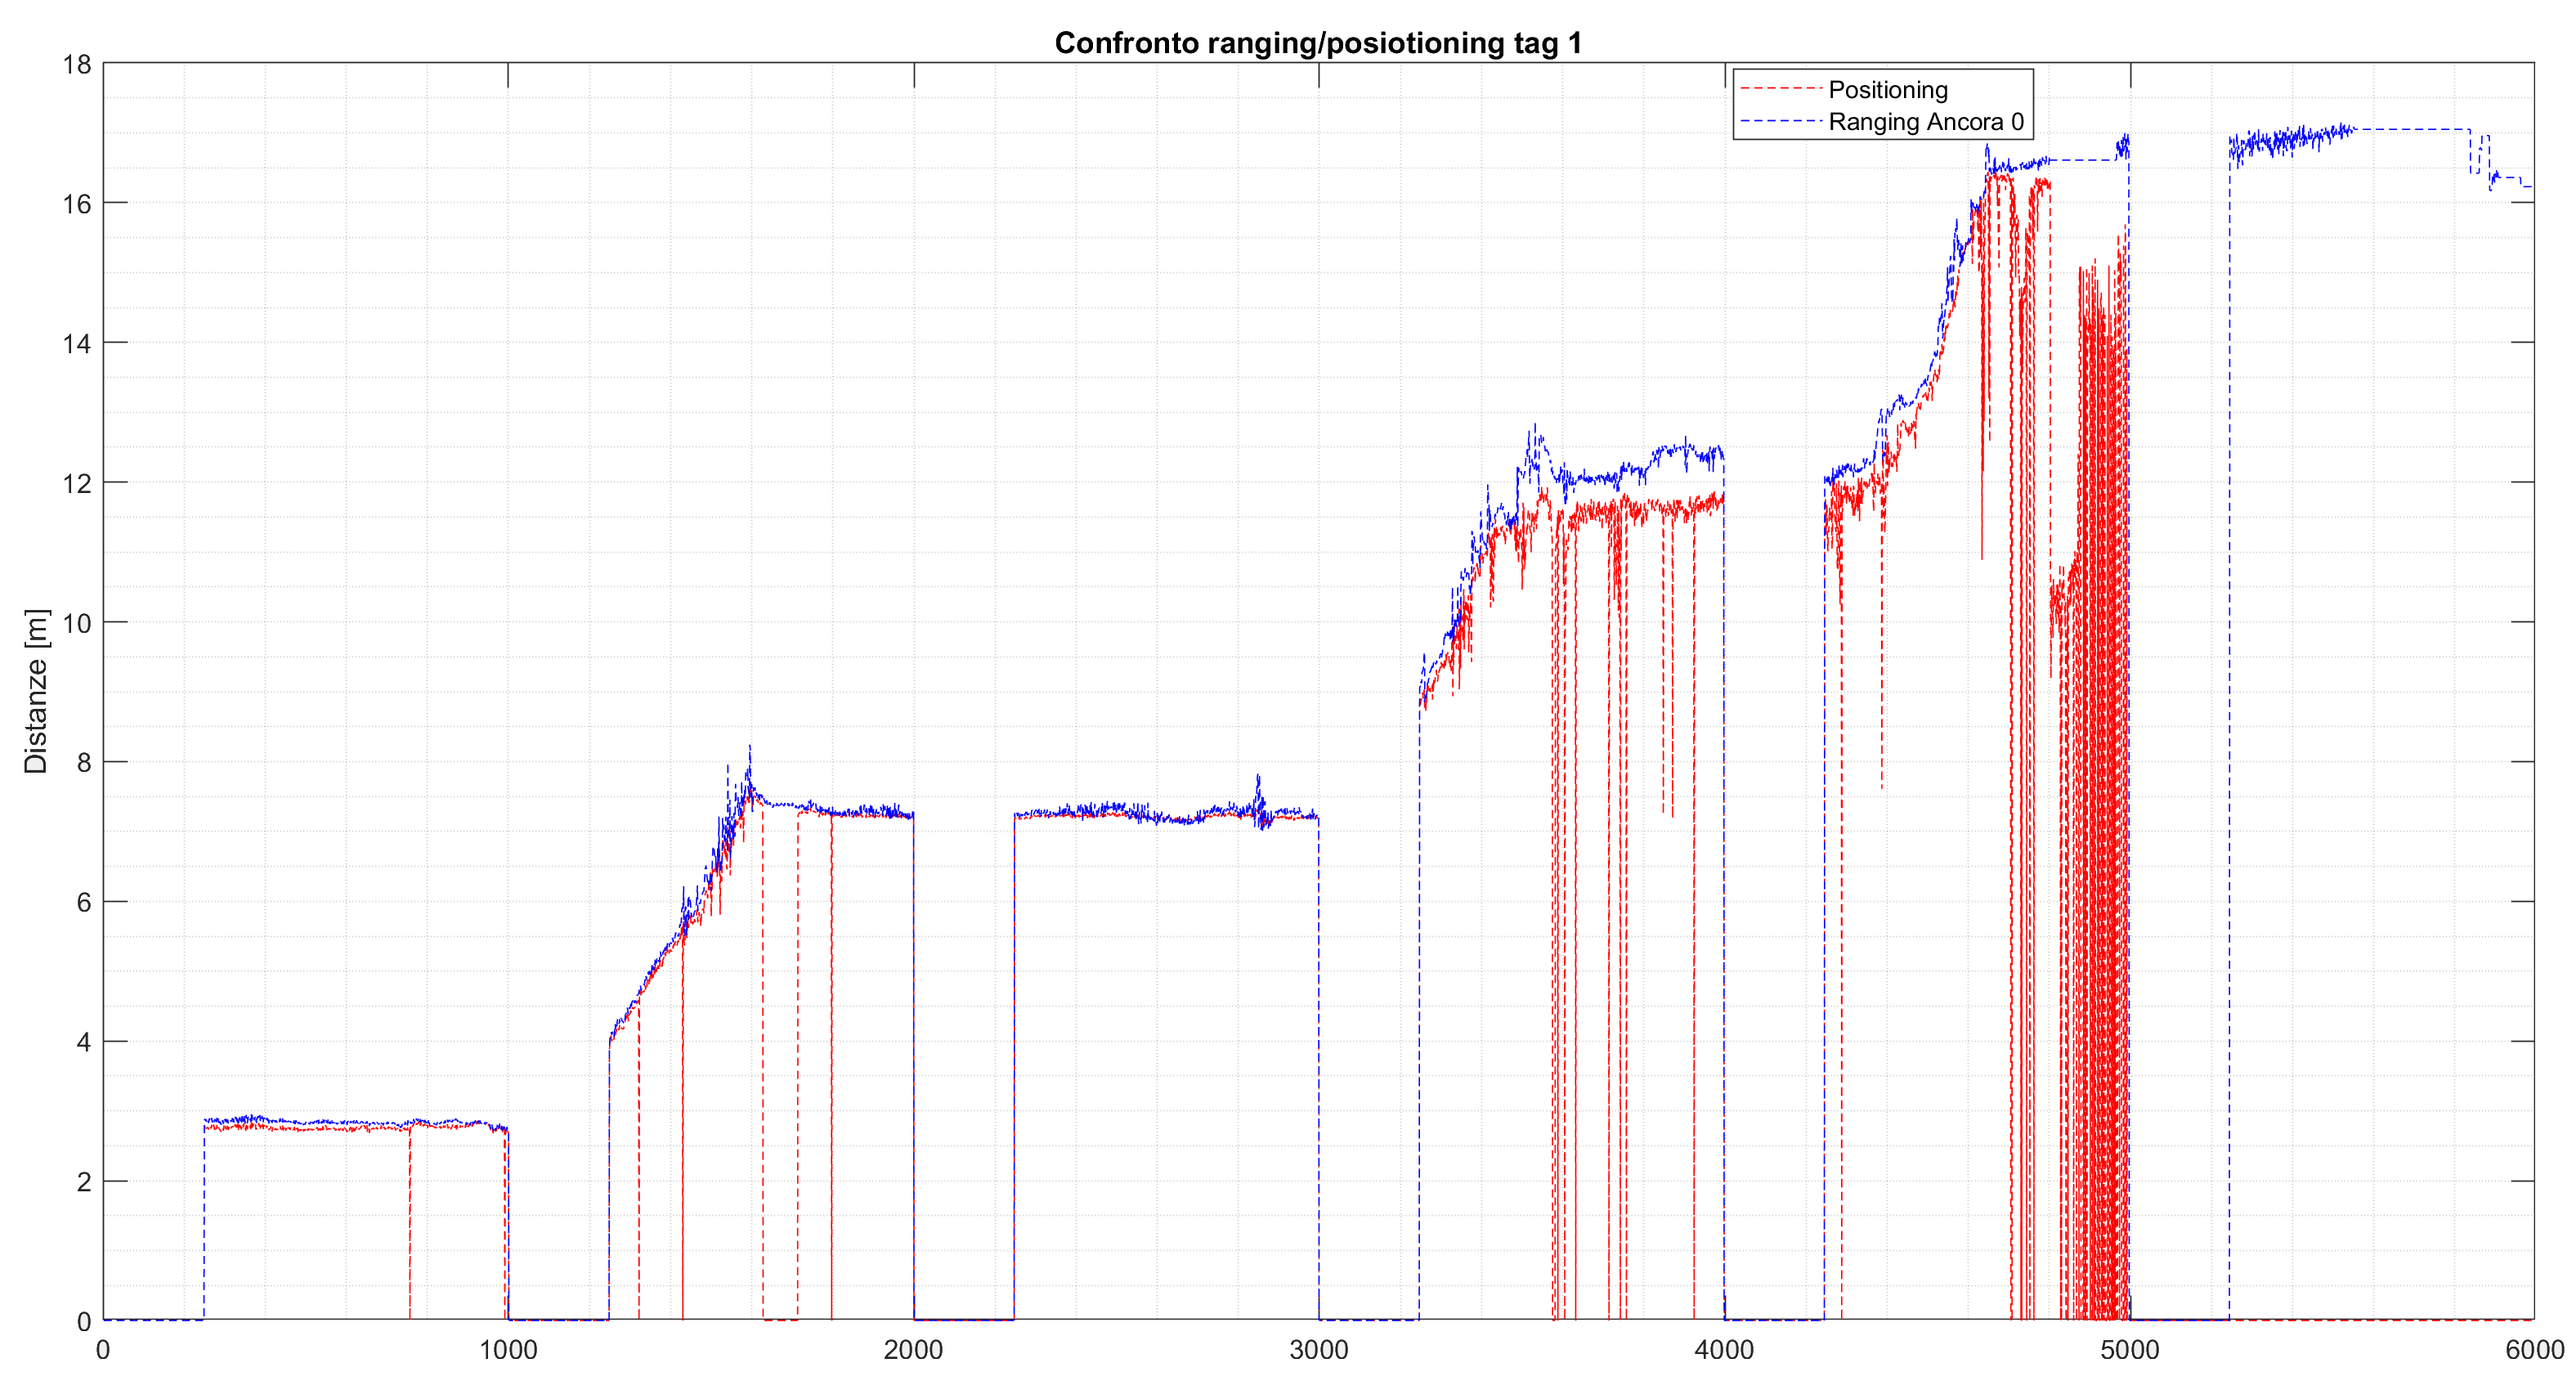
\includegraphics[scale=0.18]{PosRangTag1}
			\caption{\textbf{Figura 30:} confronto ranging/positioning tag 1\label{PosRangTag1}}
		\end{figure}
		\begin{figure}[H]
			\centering
			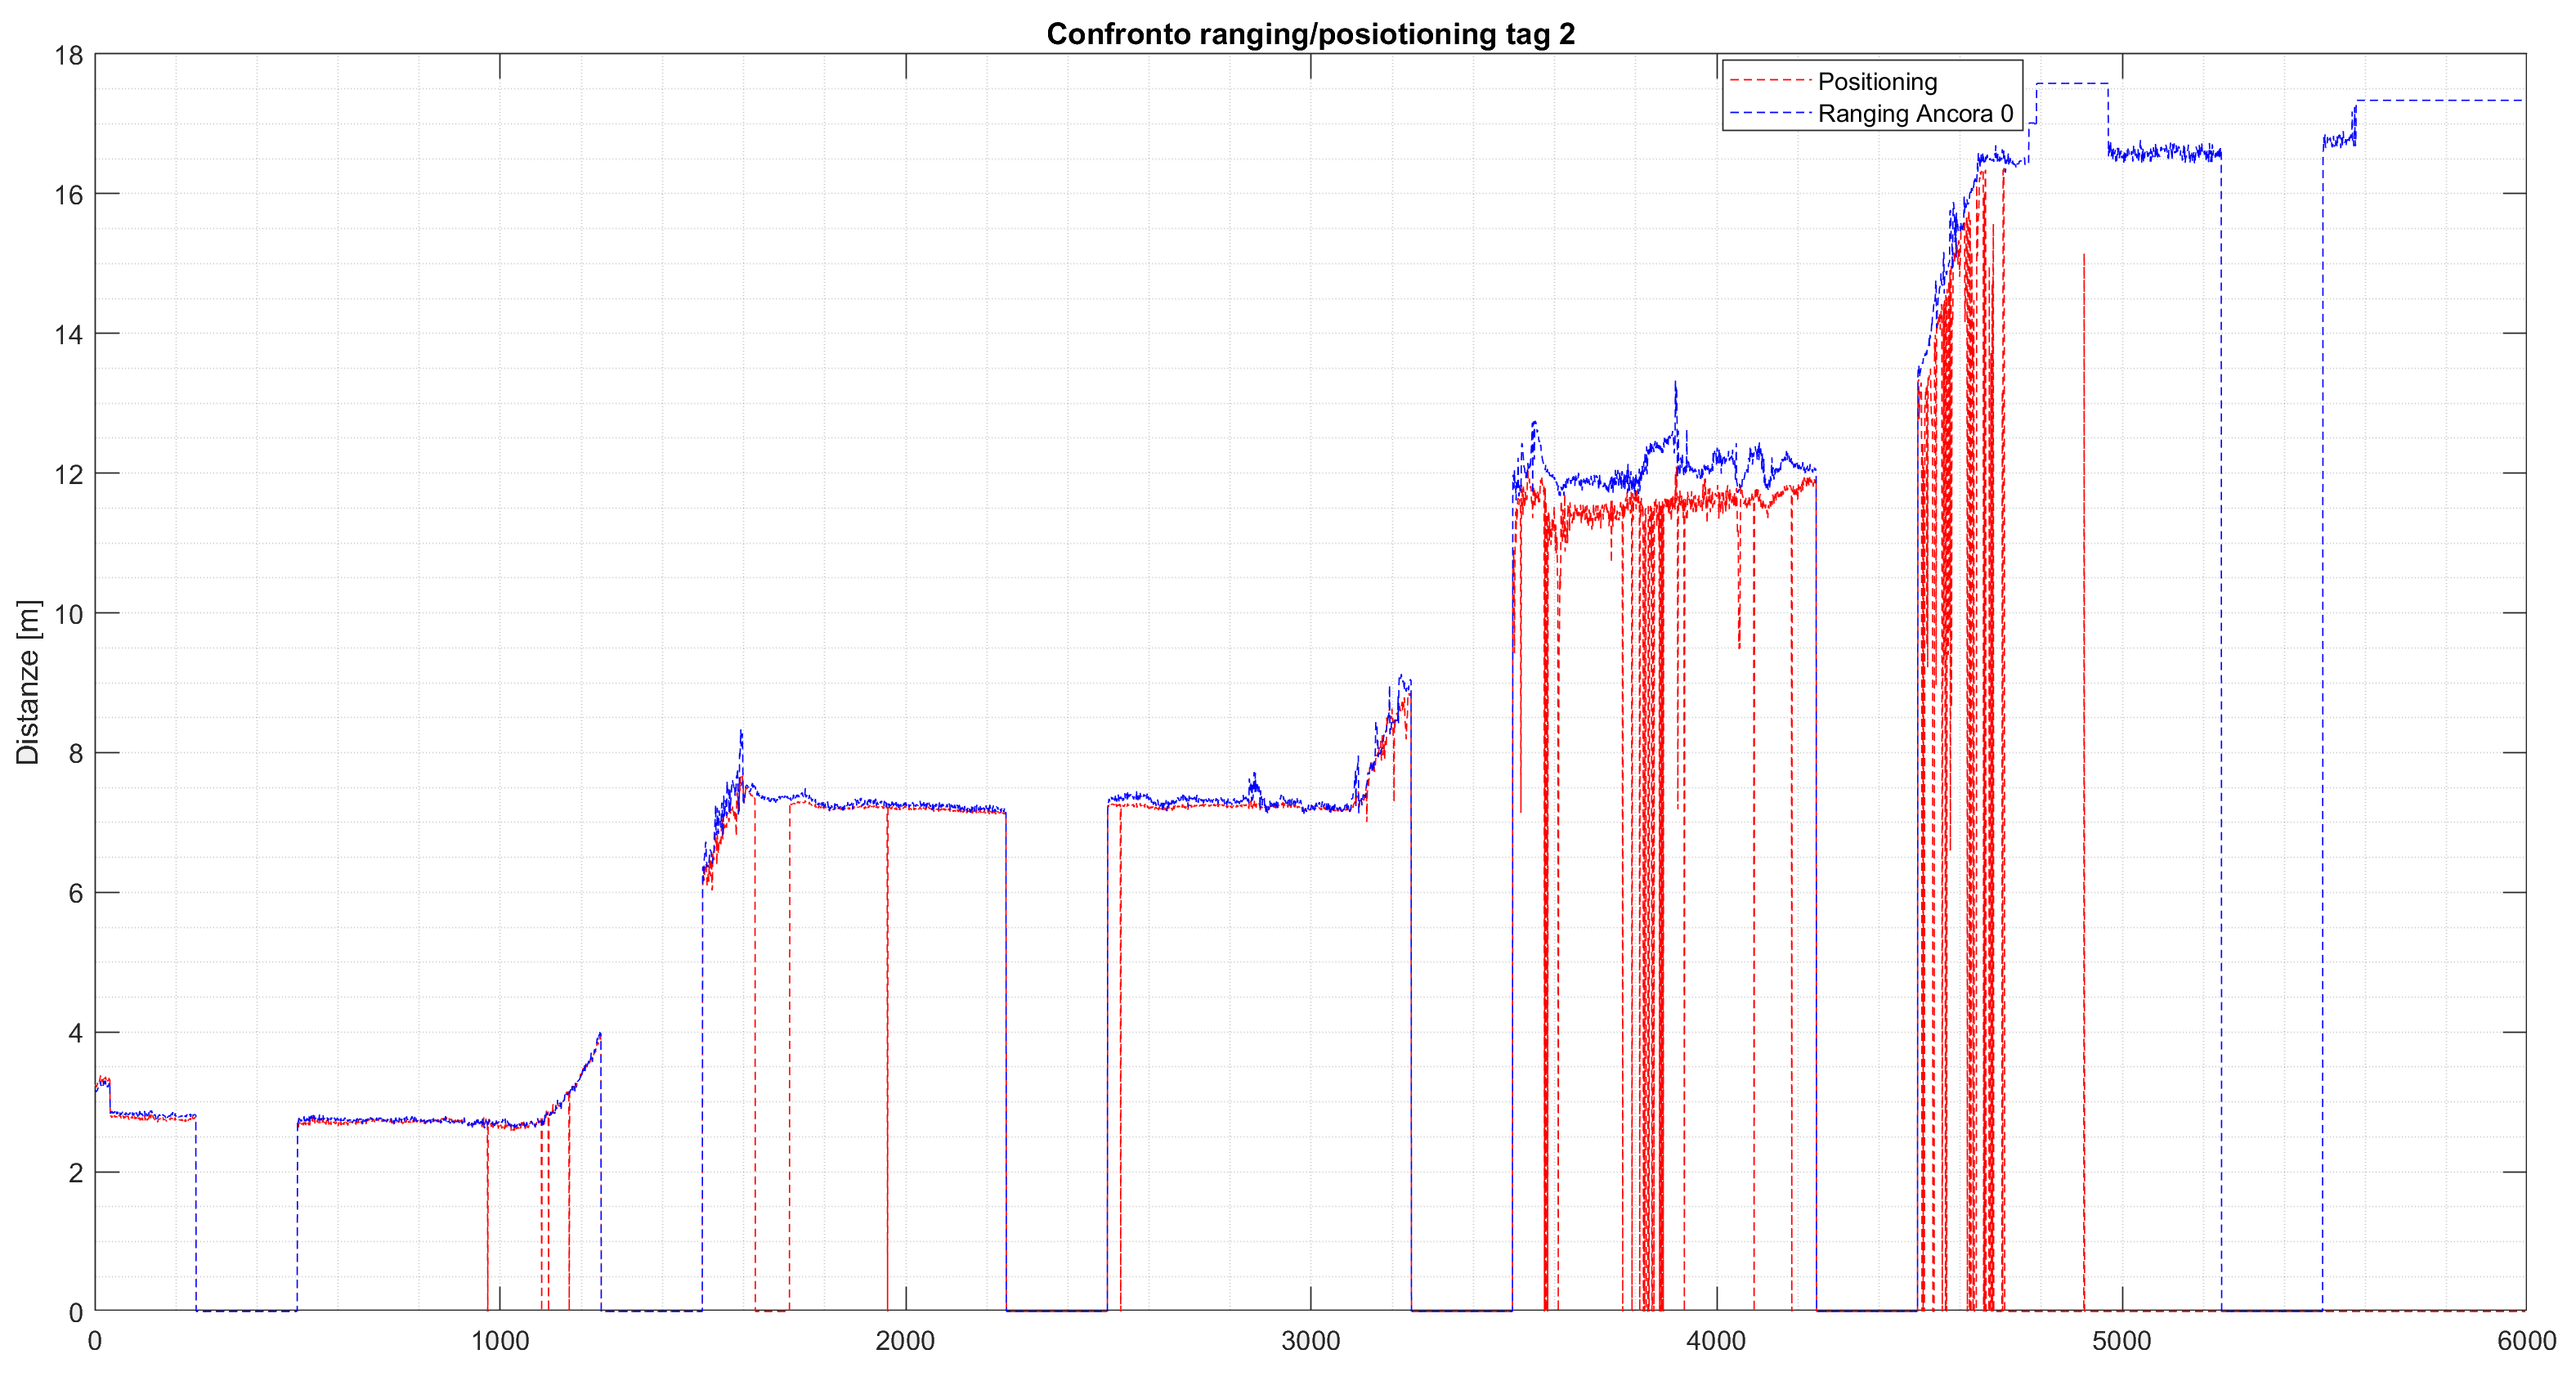
\includegraphics[scale=0.18]{PosRangTag2}
			\caption{\textbf{Figura 31:} confronto ranging/positioning tag 2\label{PosRangTag2}}
		\end{figure} 
		In conclusione, il sistema Pozyx, sembrerebbe essere discretamente affidabile a piccole distanze dalle ancore per precisione, accuratezza e percentuale di fallimenti. Man mano che ci si allontana da esse, il tag rileva misure poco accurate e il numero di fallimenti aumenta. Si considerano fallimentari sia i casi in cui 				l’algoritmo di doPositioning non converge che quelli in cui vengono restituite coordinate nulle. Poiché l’algoritmo con cui Pozyx effettua la trilaterazione, non viene reso pubblico, non si riesce a comprendere quale sia la condizione per cui doPositioning potrebbe non convergere nonostante i ranging non sembrino 				affetti da eccessivo rumore e, nei casi in cui l’algoritmo viene definito convergente, non si comprende perché le coordinate vengano poste a zero.

	\end{section}
	\newpage

	\begin{section}{Come condurre un esperimento}
 		
		Affinchè sia possibile condurre un esperimento è necessario effettuare dei semplici passaggi. Sbagliare alcuni di essi, però, potrebbe compromettere o quanto meno peggiorare l'esito dello stesso.\\
		Viene sinteticamente riportato un elenco dei passi da compiere.
		\begin{enumerate}
				\item La prima operazione da compiere è quella di \textbf{scaricare le librerie necessarie}.\\ Buona norma è controllare che le librerie standar di Arduino siano tutte aggiornate. Oltre a queste, però, come già descritto, sarà necessario includere altre due librerie per il funzionamento del sistema:	
						la libreria \textit{"Pozyx-Arduino-library-master"} nella versione modificata per due tag; la libreria \textit{"SerialPort"}. Da notare che della libreria Pozyx esistono tre versioni: l'originale (utilizzabile solo con un tag), quella modificata per due tag e quella modificata per due tag con l'utilizzo della  libreria 									\textit{"SerialPort"}. Andrà inclusa quest'ultima oppure modificare gli sketch per l'utilizzo della seriale standard. 
				\item Entrambe le librerie dovranno essere \textbf{incluse tra quelle di Arduino}. Per far ciò si può o copiare direttamente le cartelle nella posizione $C:\setminus...\setminus Arduino\setminus libraries$, oppure selezionarle dall'IDE Arduino ($Sketch>\#includi$ $libreria>Aggiungi$ $libreria$ $da$ $file 										.ZIP…$). Bisogna anche ricordarsi di fare comunque l'\textit{include} delle librerie all'inizio dello sketch. Oltre queste due andrà inclusa anche la libreria \textit{Wire} per la comunicazione I$^2$C.
					\begin{figure}[H]
						\centering
						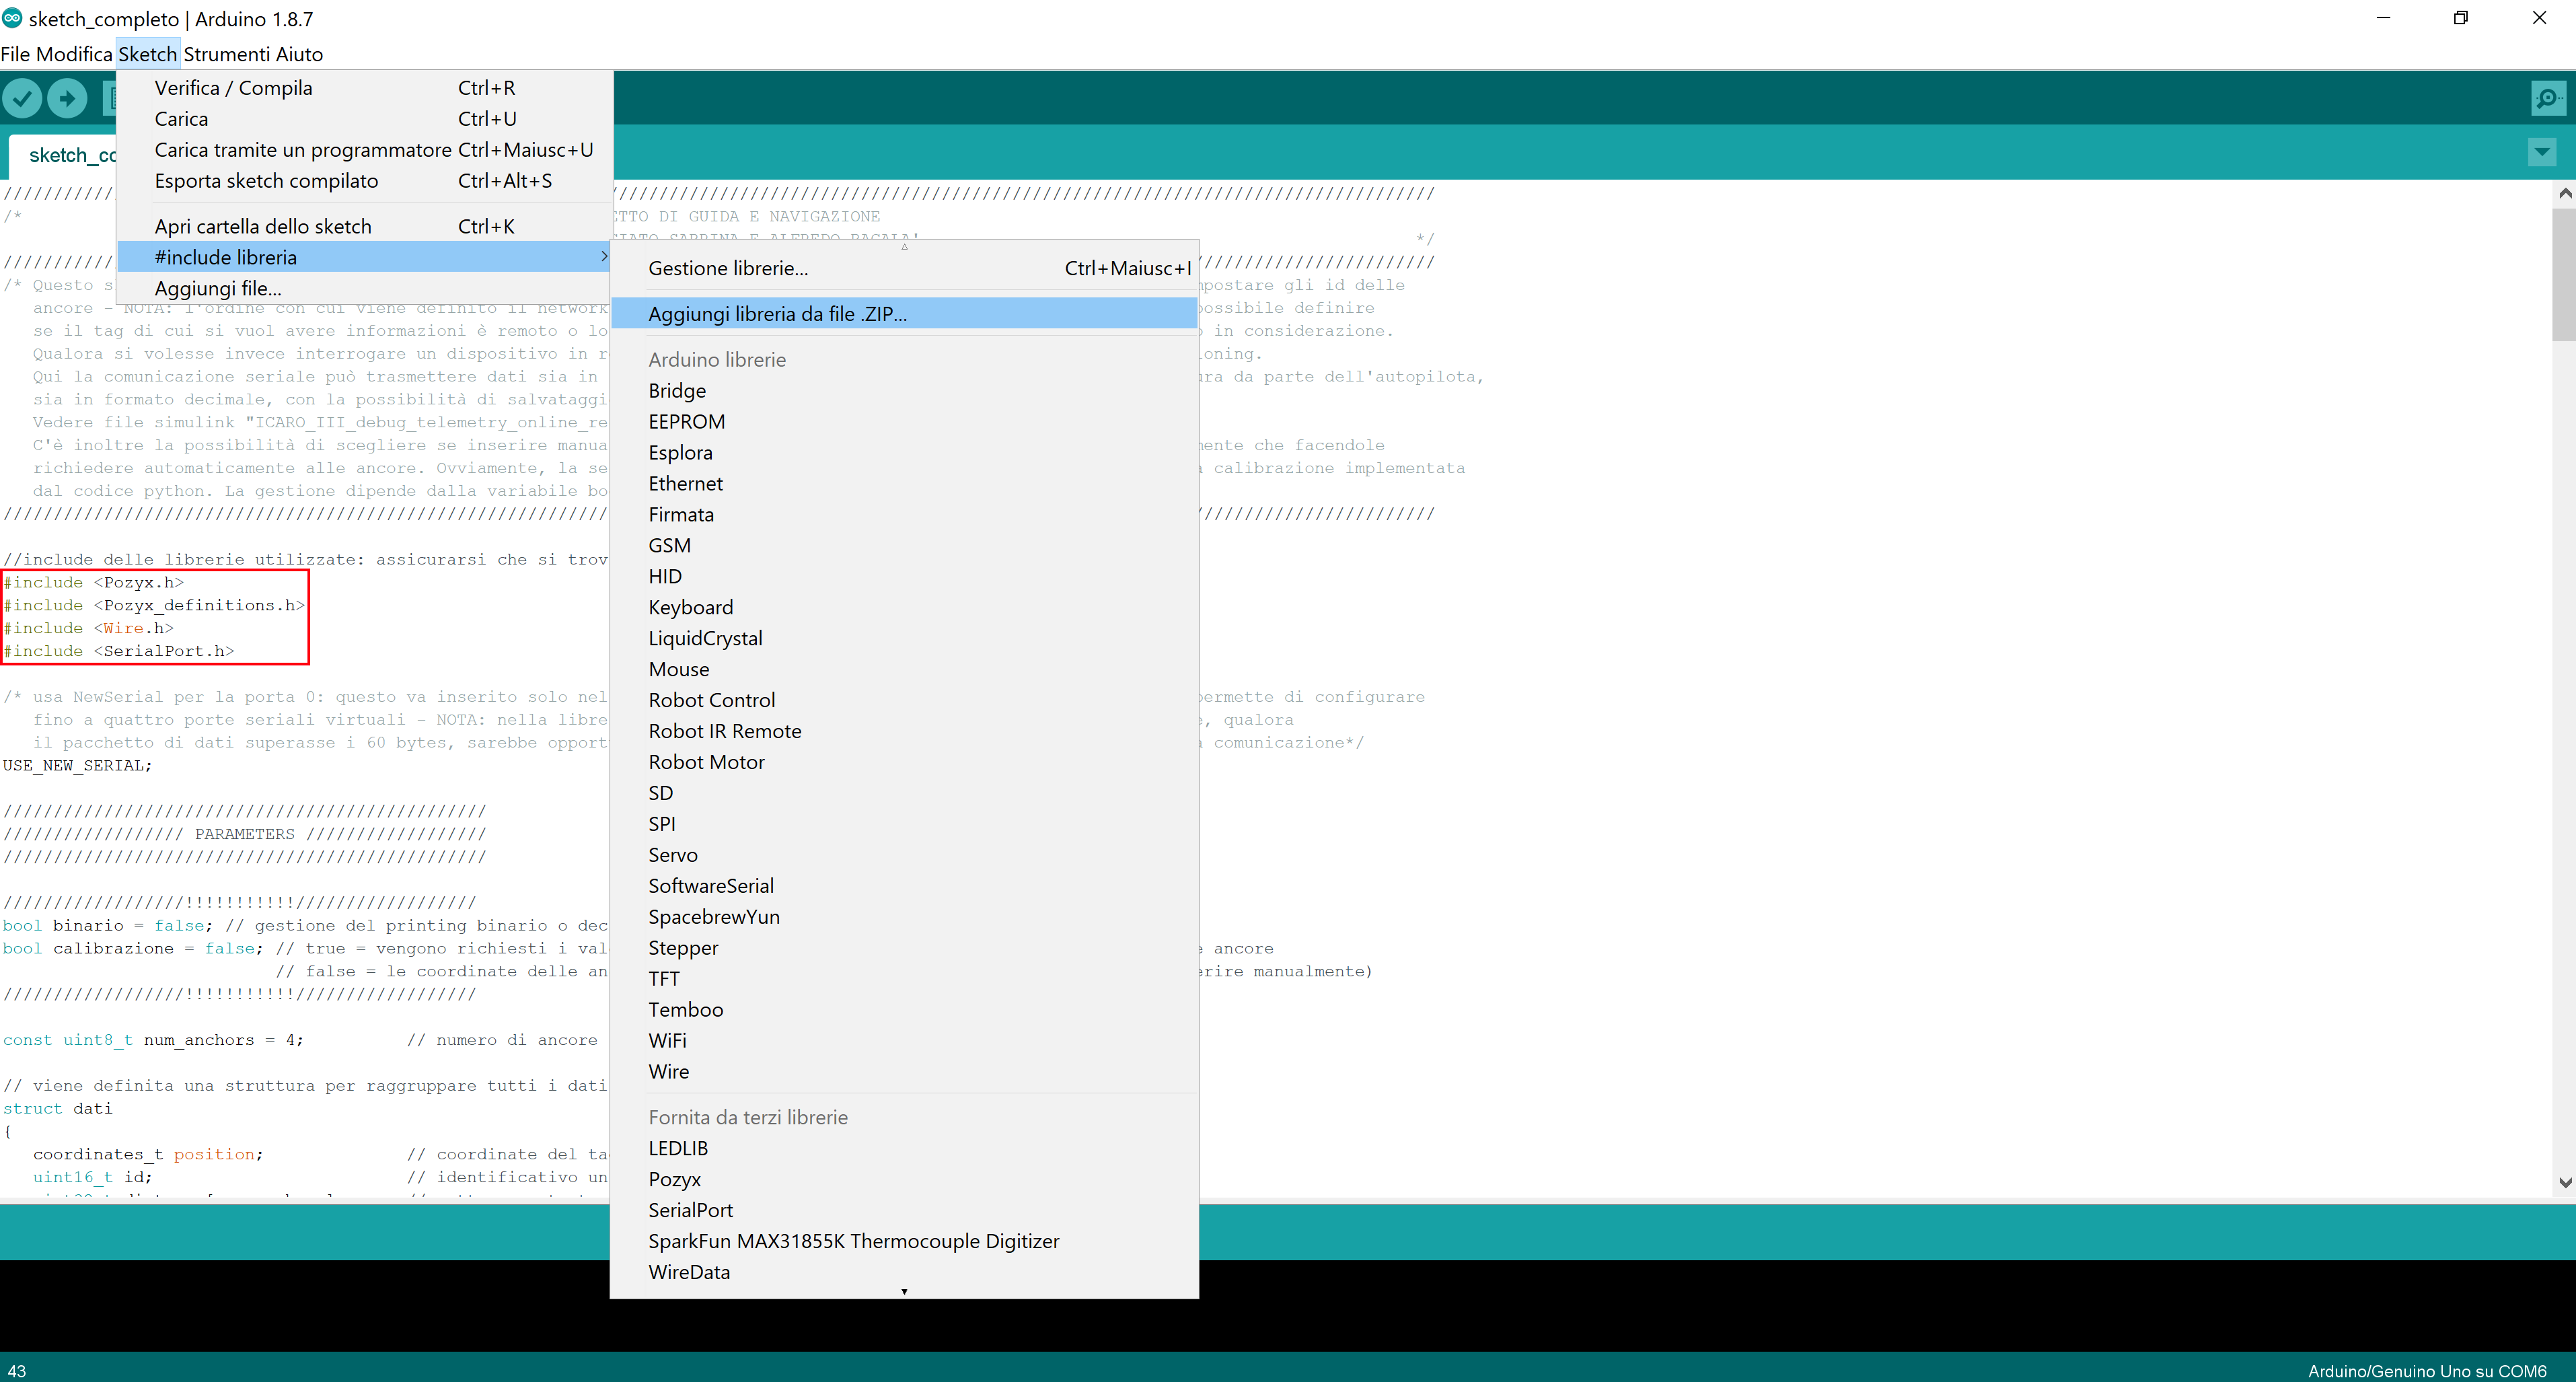
\includegraphics[scale=0.15]{Cattura}
						\caption{\textbf{Figura 32:} inclusione delle librerie\label{Cattura}}
					\end{figure} 
				\item Bisogna prestare attenzione al \textbf{posizionamento delle ancore}. Le principali regole sono che non devono essere tutte posizionate su una linea e che, qualora si volesse effettuare una trilaterazione 3D, un'ancora andrà piazzata su un piano differente dalle altre tre (\textbf{\figurename~												\ref{RegPos}}). Nel posizionamento bisogna prestare attenzione all'ordine con cui, a livello software, esse sono state ordinate. Dalla loro successione scaturisce, infatti, la definizione del SdR secondo la convenzione POZYX (origine definita dall'ancora 0; y: definita dall'ancora 1; z: verso l'alto), come 									indicato in \textbf{\figurename~\ref{PosAncors}}.
					\begin{figure}[H]
						\centering
						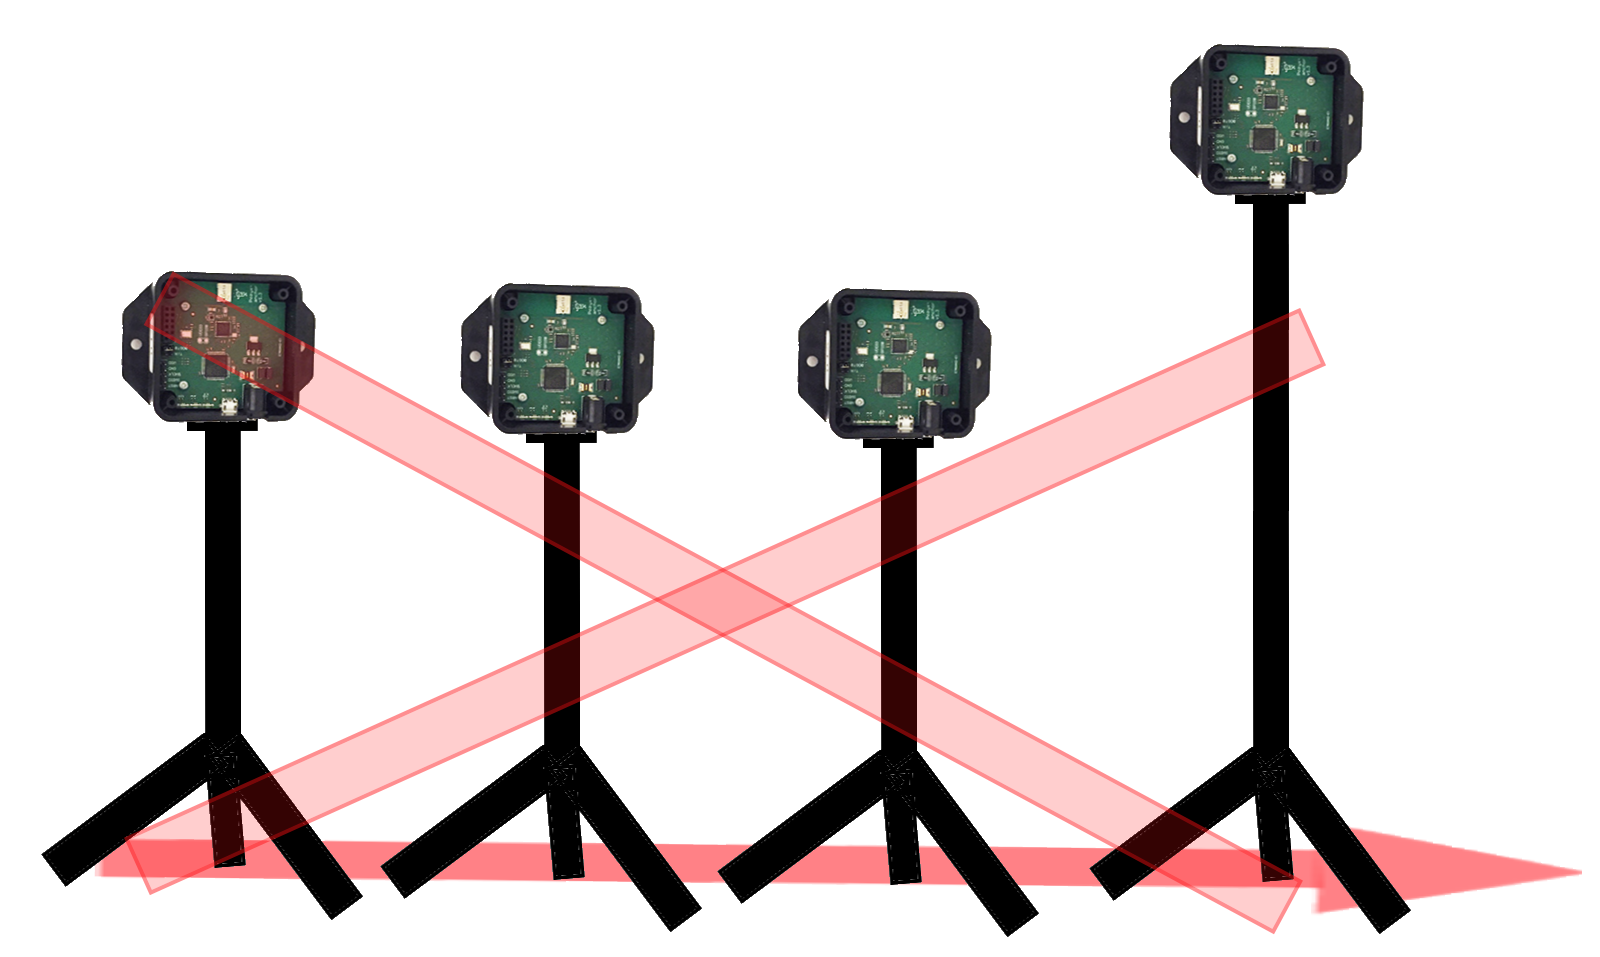
\includegraphics[scale=0.2]{NoLine}
						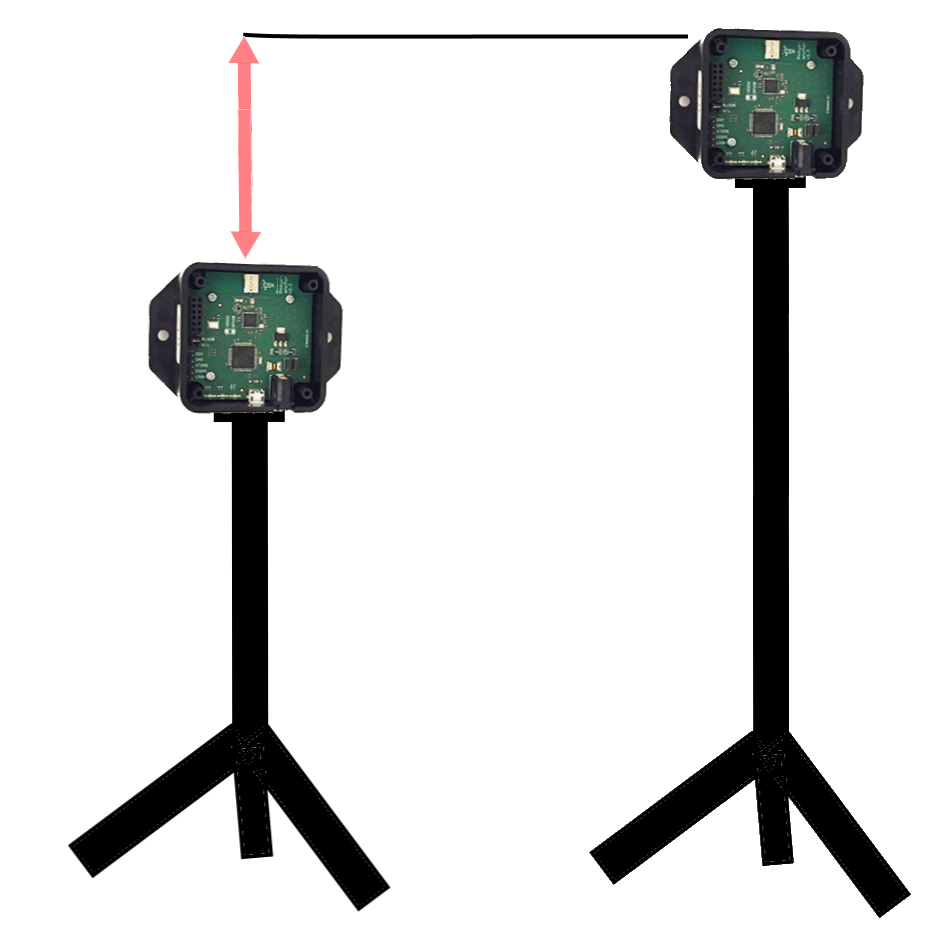
\includegraphics[scale=0.2]{DiffAncors}
						\caption{\textbf{Figura 33:} Regole posizionamento ancore\label{RegPos}}
					\end{figure} 
					\begin{figure}[H]
							\centering
							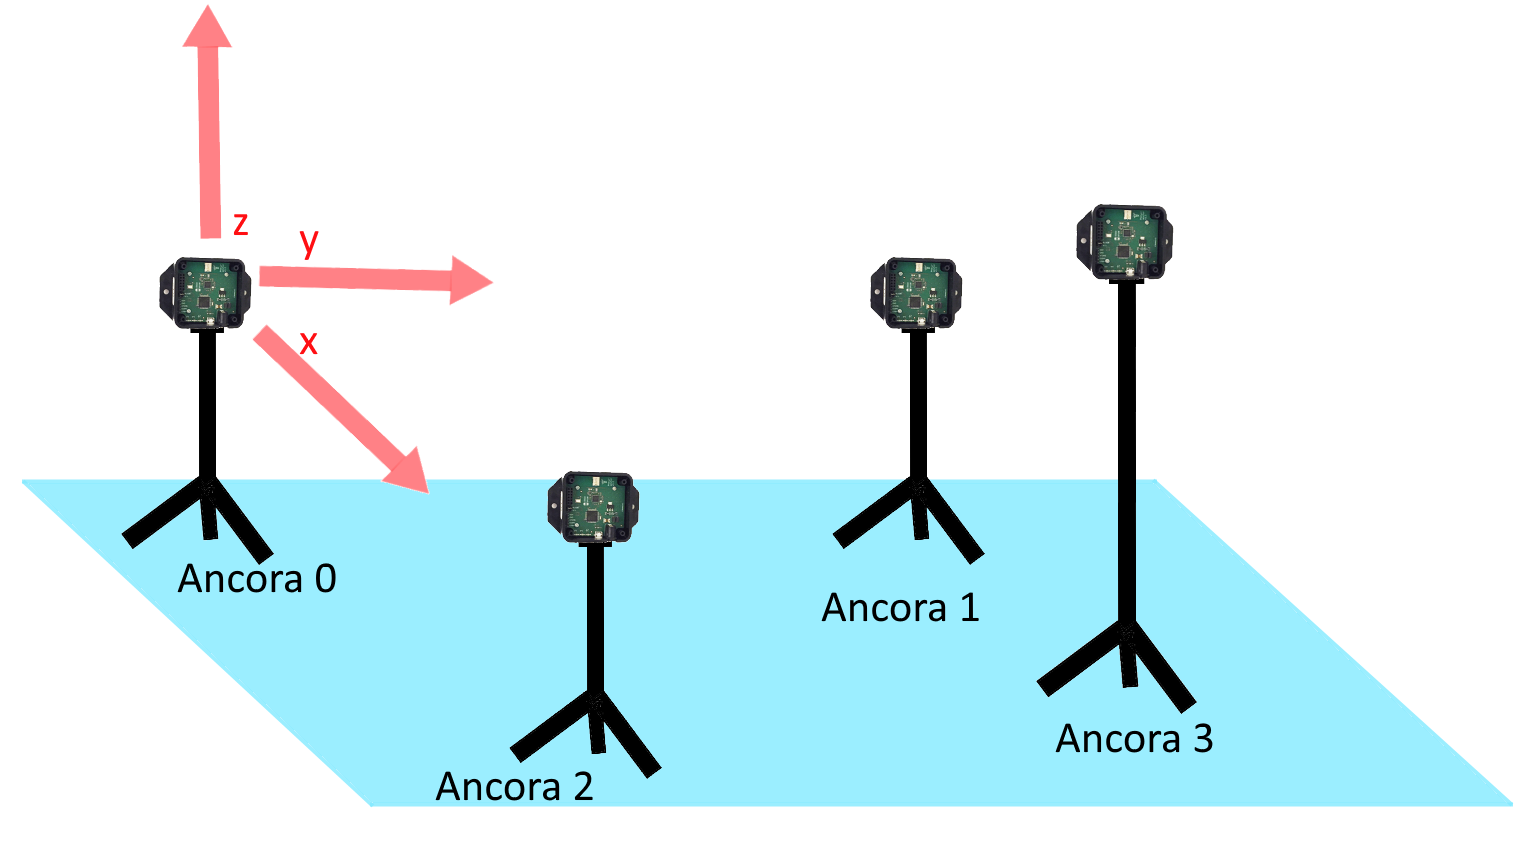
\includegraphics[scale=0.35]{PosAncors}
							\caption{\textbf{Figura 34:} SdR secondo la convenzione POZYX \label{PosAncors}}
						\end{figure} 
				\item Una volta posizionate le ancore, sarà il momento di \textbf{calibrarle.} La calibrazione consiste in un processo ripetuto di ranging tra le ancore; dopo di che esse si autolocalizzano e descrivono le loro posizioni tramite coordinate nel SdR che si viene a creare. Questo processo è implementato su un 									codice python (\textit{"autocalibration\_ransac.py"}). Tramite tale codice, bisognerà dapprima impostare i parametri UWB desiderati, e poi scegliendo tra autocalibrazione o calibrazione manuale, lanciare il codice. Quest'ultima opzione presuppone una conoscenza delle distanze tra le ancore, le quali 									andranno inserite manualmente. Una volta che la calibrazione sarà andata a buon fine, verrà richiesto se si desidera salvare il risultato nelle ancore. Bisognerà selezionare si ("y") in modo che tali misure siano successivamente disponibili per l'esperimento. \\L'esecuzione del codice richiede un tag 										connesso tramite porta seriale al computer, il cui Id (unico) andrà inserito nella variabile $serial\_id$ (riga 507 del codice); nella riga successiva, andranno inseriti gli Id delle ancore ($anchors\_id$) - si ricorda nuovamente che la successione con cui vengono inserite deve seguire la convenzione Pozyx.
				\item A questo punto si può passa alla parte dell'esperimento che coinvolge Arduino. Bisognerà prendere un Arduino Uno Rev3 e due tag. I tag da scegliere sono quelli con i pin già saldati, i quali (volendo) possono essere utilizzati come shield di Arduino. Inoltre, bisognerà scegliere due tag che abbiano 									indirizzi I$^2$C differenti, in modo da decidere con quale dei due comunicare. Tale differenza è dovuta a livello hardware, dalla saldatura di due pin sul retro della scheda, denominati \textit(I2C LSB). Le \textbf{connessioni} da effettuare non sono tutte, ma basta collegare 6 pin:
						\begin{itemize}
							\item SDA E SCL o i pin analogici A4 e A5 (per la comunicazione I$^2$C);
							\item i pin (digitali) 2 e 3 (per le interruzioni);
							\item 5V e GND (per l'alimentazione).
						\end{itemize}
						In \textbf{\figurename~\ref{Connessioni}} vengono mostrate tali connessioni.
						\begin{figure}[H]
							\centering
							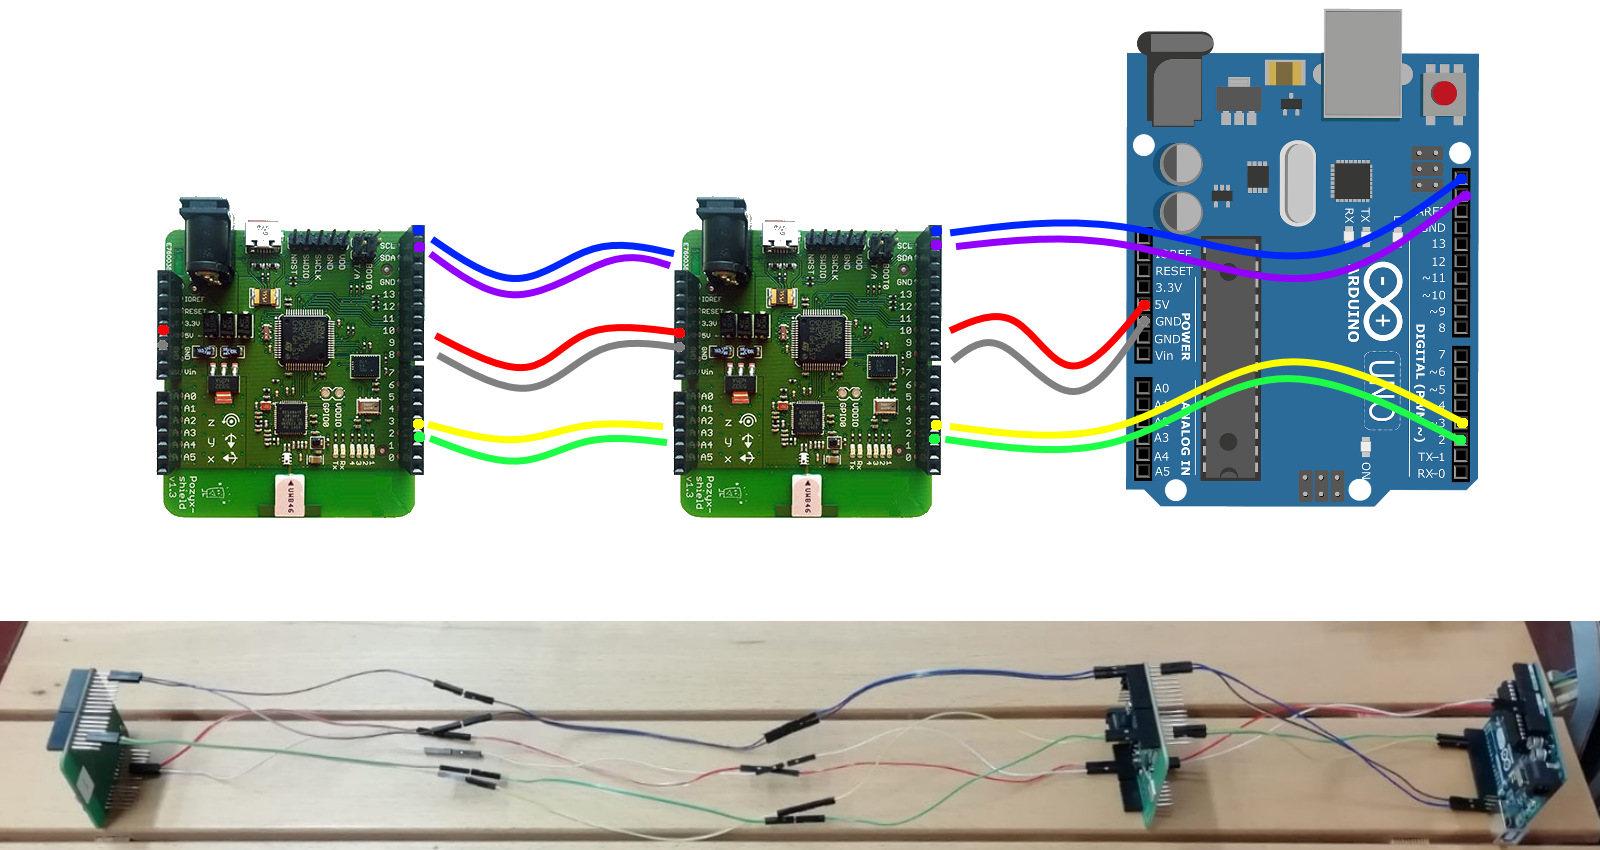
\includegraphics[scale=0.35]{Connessioni}
							\caption{\textbf{Figura 35:} Connessioni tra Arduino e due tag\label{Connessioni}}
						\end{figure} 
				\item A questo punto è necessario controllare, o cambiare a piacimento, i \textbf{parametri UWB} salvati nella memoria dei singoli device. Bisogna prestare attenzione al fatto che, per poter comunicare, i device devono avere gli stessi settaggi! Inoltre,  ogni combinazione ha potenzialmente degli effetti 										sull'esito dell'esperimento. Questa operazione andrà eseguita tramite lo sketch Arduino $pozyx\_UWB\_configurator$. Esso permette, una volta ricercati i device nelle vicinanze, di cambiarne i parametri manualmente. Da notare come, possa capitare che un device non venga trovato. Questo errore ha 										tendenzialmente tre cause: l'antenna non è alimentata; l'antenna è andata in stand-by; un errore nella comunicazione.\\ Dai test condotti i parametri ottimali riscontrati sono i seguenti:
						\begin{itemize}
							\item \textbf{channel} =  $5$; 
							\item \textbf{bitrate} =  $6810kbit/s$; 
							\item \textbf{plen} = $64 symbols$;
							\item \textbf{prf} = $64MHz$
						\end{itemize}
				\item Solo una volta espletata l'operazione precedente di setting dei parametri potrà essere settato anche il \textbf{gain}. Questo perchè i dispositivi sono progettati in maniera tale per cui il cambiamento di uno qualsiasi dei parametri, porta il valore del guadagno ad essere impostato a quello di default. 									L'assegnamento del valore di \textbf{gain} viene effettuato attraverso l'utilizzo dello sketch $pozyx\_gain\_configurator\_2tag$. Il parametro ottimo in termini di distanza è \textbf{gain} = 33.0; non essendoci apparenti differenze sulla precisione, si consiglia il settaggio di questo valore.
				\item La scelta dello \textbf{sketch da utilizzare} è strettamente connesso all'esperimento da condurre. Vengono forniti tre sketch. Essi permettono di effettuare le principali operazioni legate al posizionamento dei tag nello spazio. Sono di seguito brevemente elencati:
						\begin{itemize}
							\item \textit{sketch\_completo}: permette, se lo si desidera (bool calibrazione = true), di chiedere le coordinate dalle ancore post calibrazione (da effettuare con python), oppure, qualora si fosse a conoscenza delle stesse, ma non fossero salvate nei device, è possibile inserirle manualmente nei 												vettori $anchors\_x$, $anchors\_y$, $heigth$. I dati sono inviati su seriale sia in formato binario (bool binario = true) che in formato decimale. Questo sketch lancia la funzione di trilaterazione implementata dalla Pozyx ($doPositioning$) e richiede successivamente anche le distanze dalle ancore. 										Tali operazioni sono implementate per l'utilizzo di due tag. \\Nota: attualmente il codice pone a zero le coordinate qualora il positioning fallisca, ma non le distanze. È, però, già implementata una funzione ($zeroDist$) che volendo effettua la stessa operazione sulle distanze. 
							\item \textit{sketch\_case}: svolge le stesse operazione dello sketch precedente, ma i dati vengono inviati solo in formato decimale. Questo codice è utile qualora si vogliano testare più casi di configurazione nelle stesse situazioni ambientali in un unico test. Infatti il codice effettua in successione uno 											switch tra 4 casi:
									\begin{itemize}
										\item richiesta di informazioni (positioning e ranging) solo al tag con indirizzo I2C 0x4A;
										\item richiesta di informazioni (positioning e ranging) solo al tag con indirizzo I2C 0x4B;
										\item richiesta di informazioni (positioning e ranging)ad entrambi con la successione 0x4A - 0x4B;
										\item  richiesto di informazioni (positioning e ranging)ad entrambi con la successione 0x4B - 0x4A.
									\end{itemize}
									Le operazioni sono ripetute 250 volte per ogni caso.
							\item \textit{sketch\_ranging}:  questo sketch serve nel caso in cui si volesse effettuare un esperimento esclusivamente sul ranging tra un'ancora e i due tag in parallelo.
						 \end{itemize}
				\item Una volta lanciato lo sketch Arduino opportuno, per il salvataggio dei dati ci sono diverse possibili vie. Innanzitutto, bisogna distinguere i casi di scrittura su seriale in formato binario o decimale. \\Nel primo caso, sarà necessario caricare ed eseguire il file simulink 																							\\$ICARO\_III\_debug\_telemetry\_online\_receiver\_POXYZ\_v1slx$, il quale salva tutti i dati ricevuti una volta terminato l'esperimento. In tal caso bisogna controllare il numero di bytes inviati e inserire preventivamente tale valore nel file stesso. Nel caso in cui, invece, la scrittura sia in formato 										decimale è possibile accedere direttamente al Serial Monitor di Arduino e una volta finito, copiare da tale schermata i dati e salvarli in un file .txt. In alternativa viene fornito uno sketch, scritto tramite l'utilizzo del programma Processing 3, denominato "\textit{salva\_simula}". Questo permette sia un 									plotting in tempo reale dei dati che un salvataggio delli stessi. Prima di lanciare questo codice bisognerà, però, trascrivere le coordinate delle ancore ed i nomi da dare al file .txt ed all'immagine che verranno poi salvati. Ci sono anche una serie di parametri grafici modificabili, come il valore di offset 									delle ancore che le sposterà nella schermata, o la scala utilizzata.
				\item Infine, una volta ottenuti i dati, sarà possiibile analizzarli. Un'alternativa proposta è quella di utilizzare il codice matlab fornito. Per la sua fruizione è necessario seguire il seguente formato:
						\begin{table}[H]
							\centering
\resizebox*{1.0\textwidth}{!}{
							\begin{tabular}{|c|c|c|c|c|c|c||c|c|c|c|c|c|c||c|c|c|c|}
								\hline
								\multicolumn{7}{|c||}{Tag 1}& \multicolumn{7}{|c||}{Tag 2}& \multirow{2}{*}{status}& \multirow{2}{*}{errore}& \multirow{2}{*}{tempo}& \multirow{2}{*}{caso}\\
								\cline{1-14}
								\multicolumn{3}{|c|}{Coordinate}& \multicolumn{4}{|c||}{Distanze}& \multicolumn{3}{|c|}{Coordinate}& \multicolumn{4}{|c||}{Distanze}&&&& \\
								\hline
								 x& y& z& dist0& dist1& dist2& dist3&  x& y& z& dist0& dist1& dist2& dist3& \{0,1,2,3\}& \{0,1,2,3\}& [ms]& \{0,1,2,3\}\\
								\hline
							\end{tabular}
}
						\end{table}
 						Qualora, alcuni dei dati qui riportati non venissero utilizzati e/o salvati durante l'esperimento, sarà necessario porre a zero la variabile corrispondente nel codice matlab. Il file principale, nonchè quello da lanciare per tutta l'analisi, è  "$AnalizzaEsperimento.m$", dove si trovano anche le variabili appena 								citate ed alcuni altri parametri modificabili. Lo script e le funzioni restituiscono dei plot per l'anailisi grafica (plottaggio di un set di distanze tramite medie e deviazioni, confronto distanze calcolare e reali, confronto della distanza dall'ancora zero calcolata tramite ranging e positioning, confronto delle 									distanze rispetto allo status e all'errore), nonchè una tabella riassuntiva con tutti i dati di interesse, compresi fallimenti e frequenza del loop Arduino.
		\end{enumerate}

	\end{section}	
	\newpage


	\section*{\hypertarget{A1}{\textbf{Allegato A - Schema circuitale Arduino Rev3}}}
	\begin{figure}[H]
		\centering
		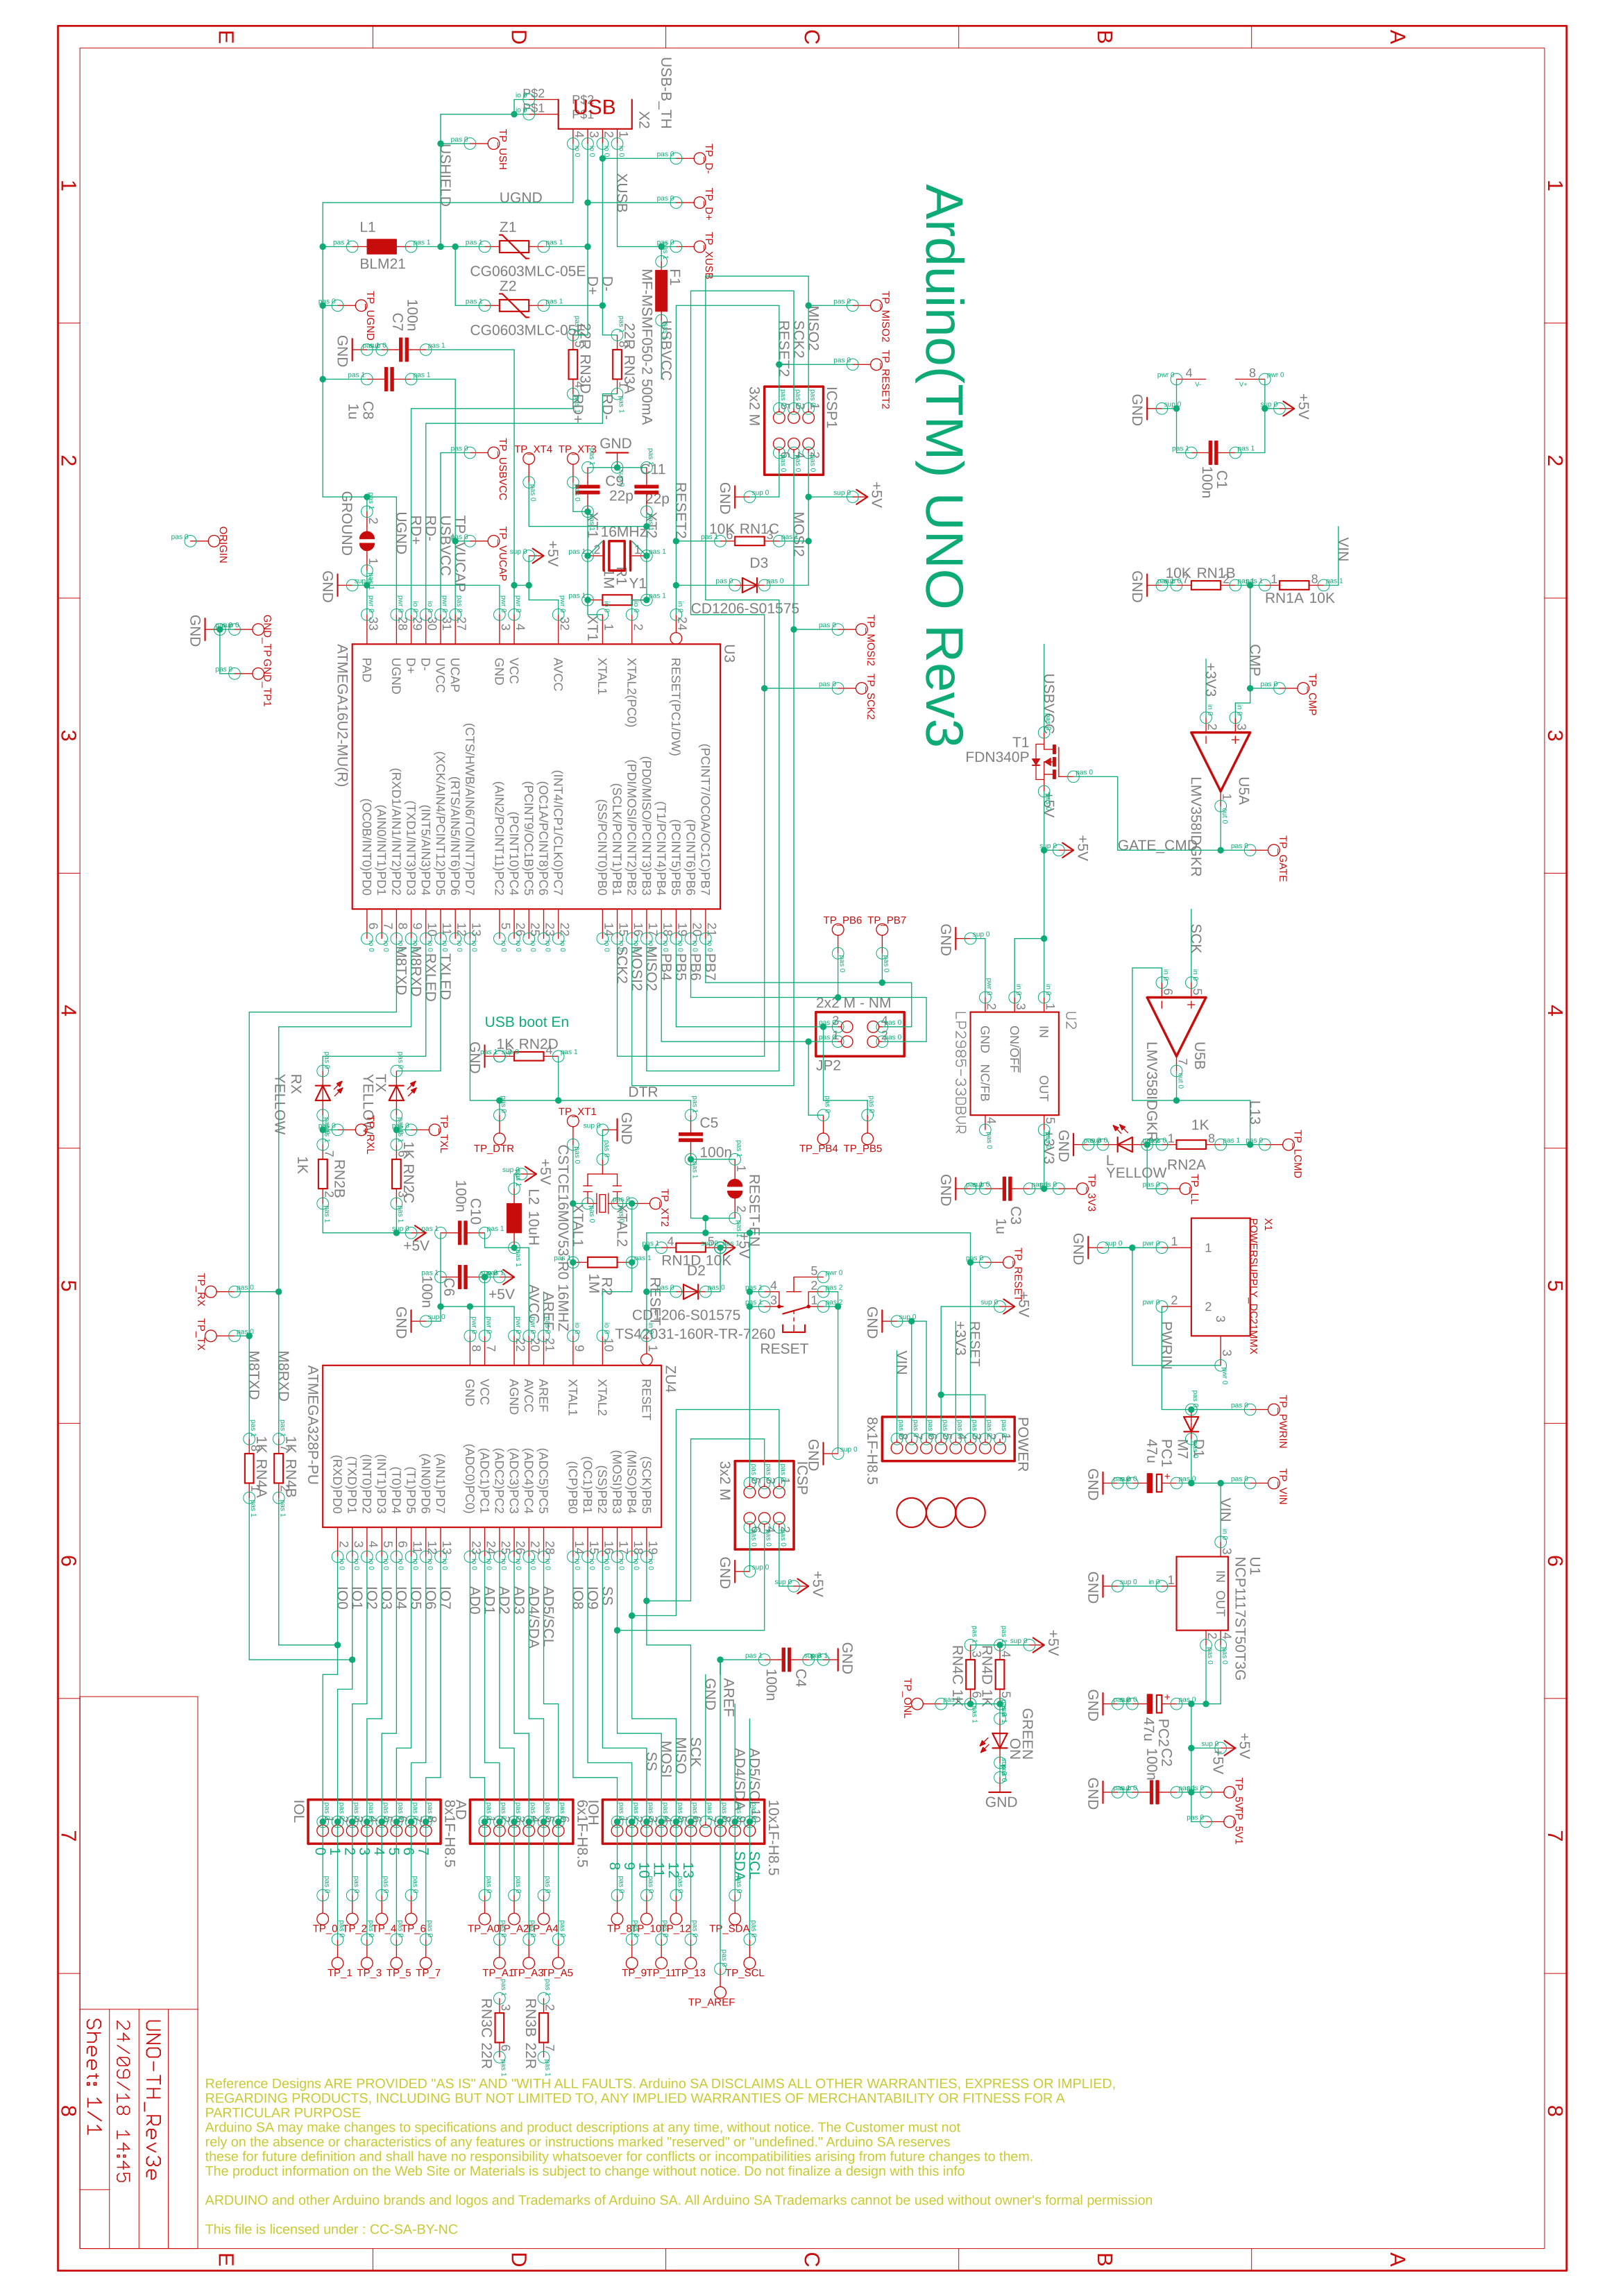
\includegraphics[scale=0.22]{UNOsch}
	\end{figure} 
	\newpage

	\section*{\hypertarget{A2}{\textbf{Allegato B - Codice su Processing 3}}}
	\lstloadlanguages{Java}
	\lstset{basicstyle=\tiny}
	\lstinputlisting{salva_simula.pde}

	\section*{\hypertarget{A3}{\textbf{Allegato C - Flowchart \textit{doPositioning}}}}
	\begin{figure}[H]

		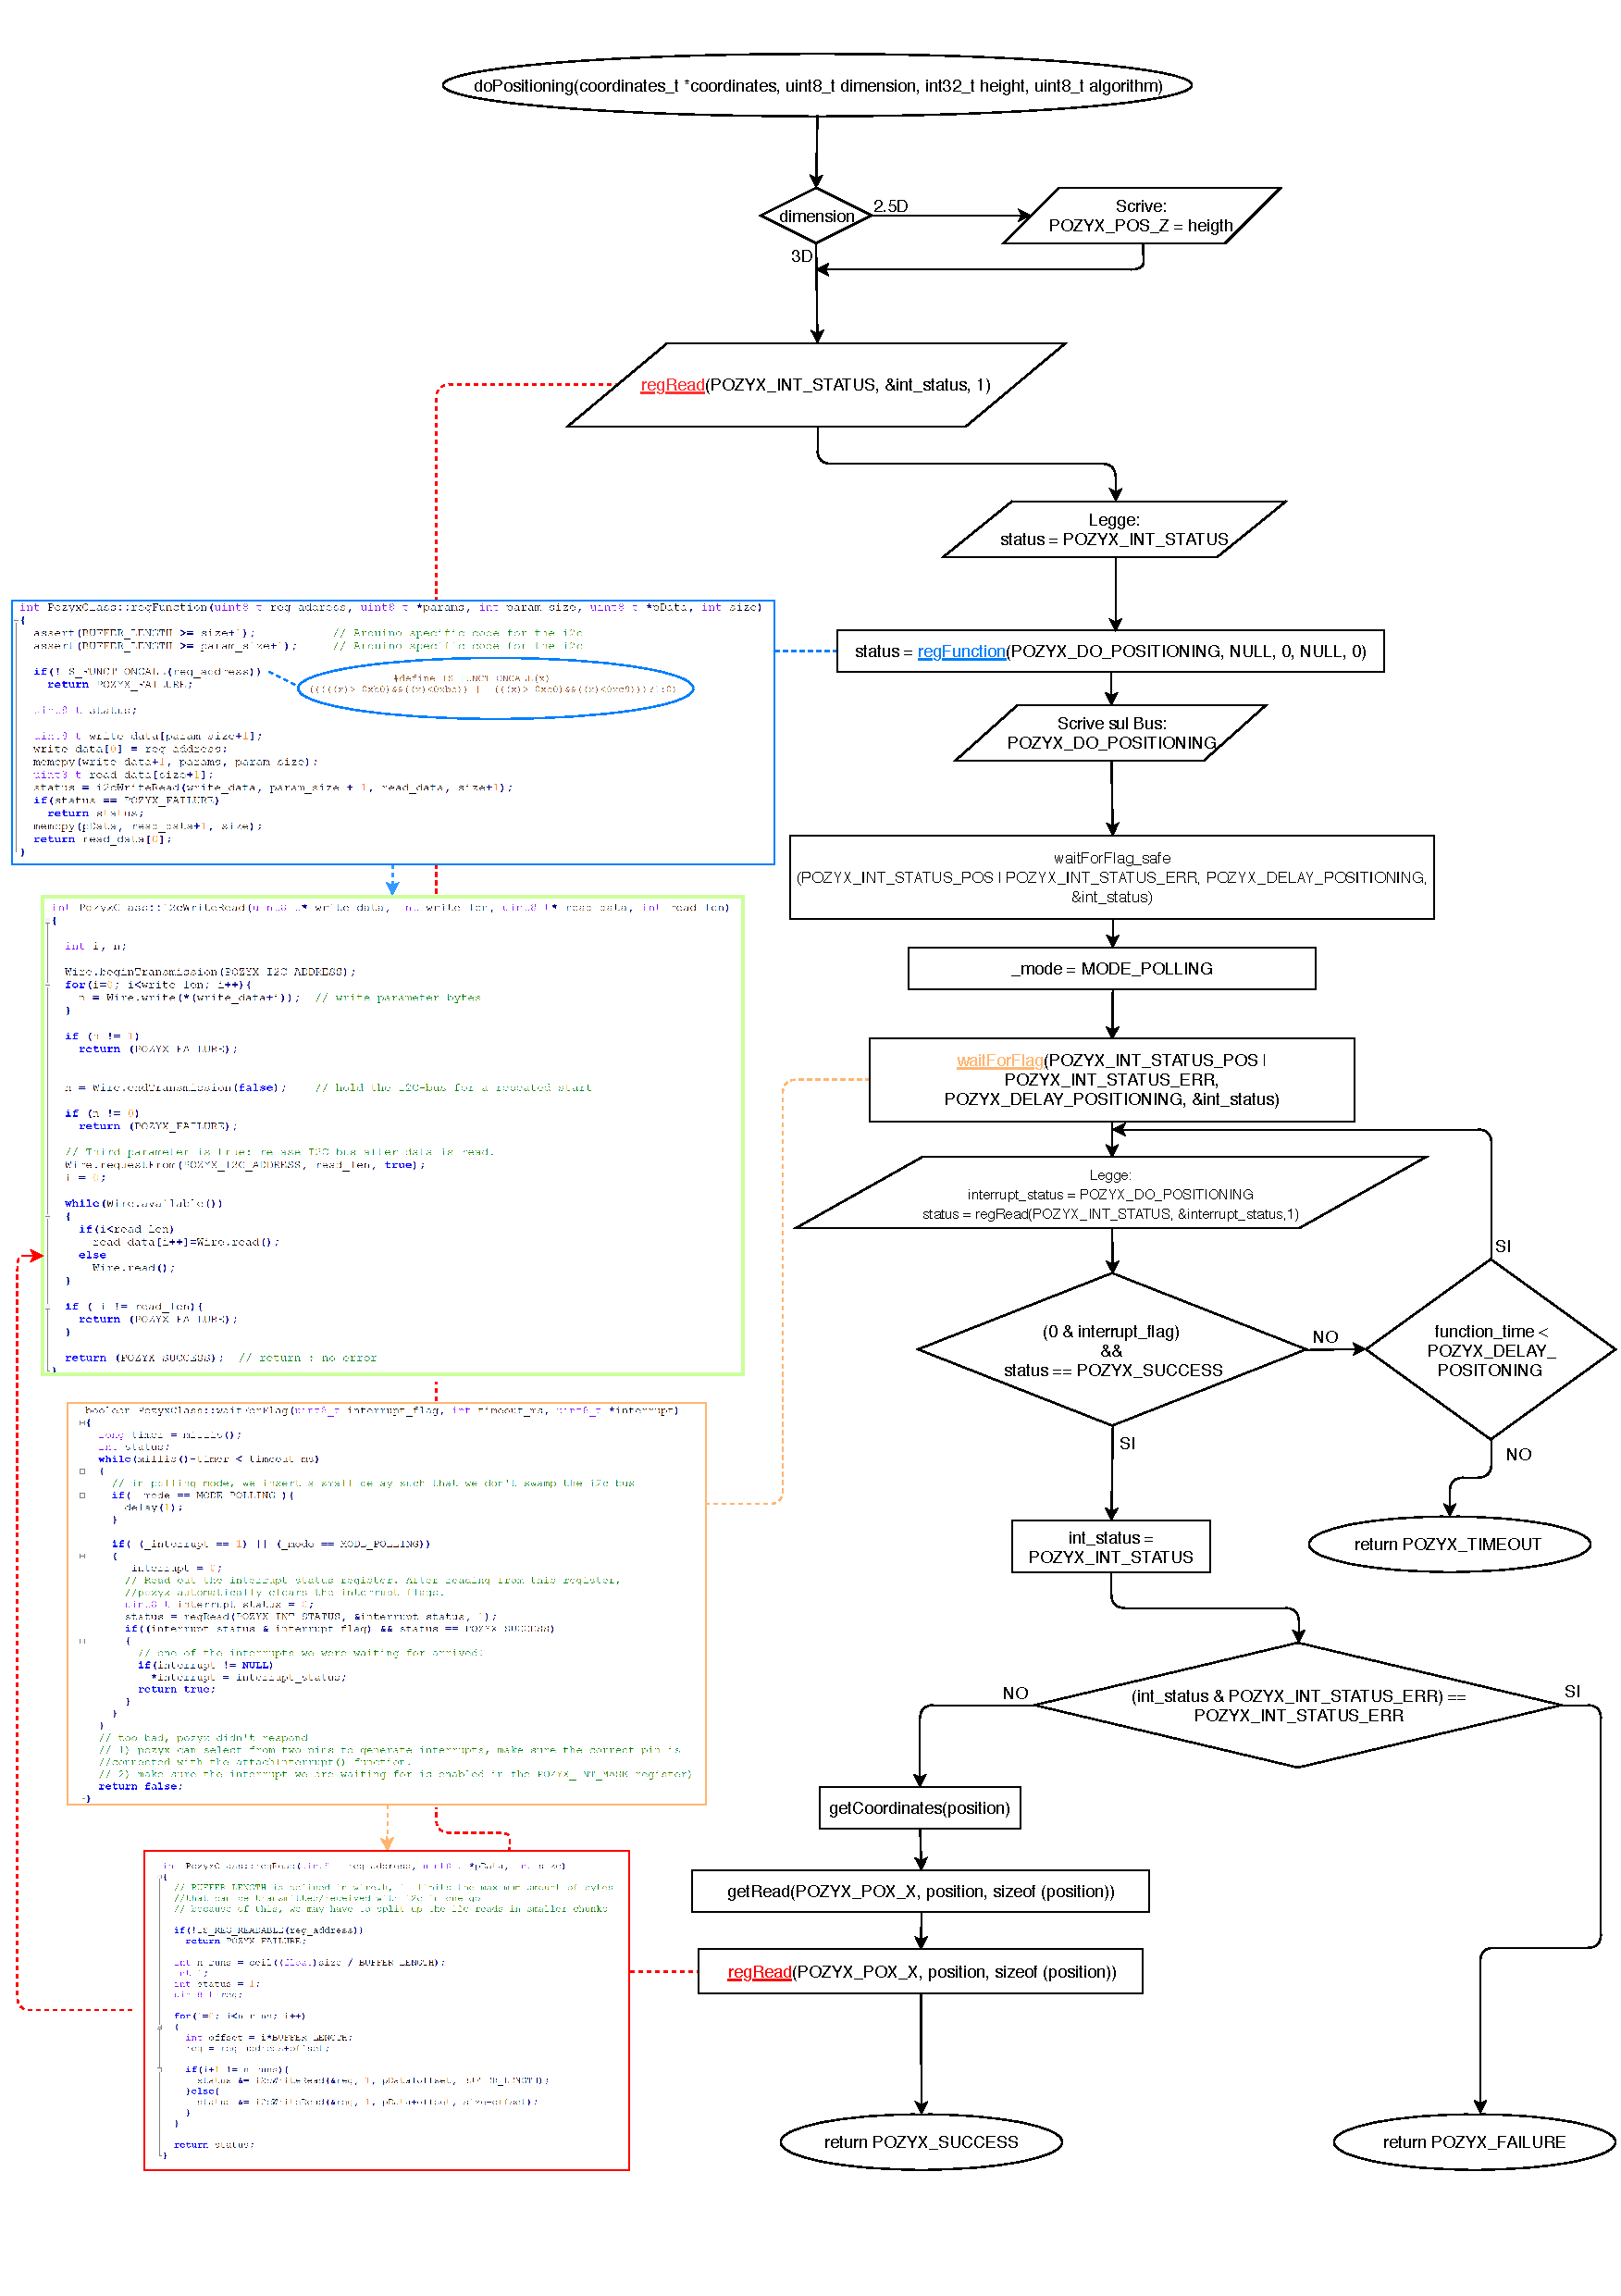
\includegraphics[scale=0.5]{flowchart_doPositioning}
	\end{figure} 
	\newpage

	\section*{\hypertarget{A4}{\textbf{Allegato D - Sketch dimostrativo Arduino}}}
	\lstloadlanguages{C}
	\lstset{basicstyle=\tiny}
	\lstinputlisting{sketch_dimostrativo.ino}
	\newpage


\bibliography{Referenze}
\bibliographystyle{plain}

\end{document}